\documentclass[a4paper, twoside]{report}

%% Language and font encodings
\usepackage[english]{babel}
\usepackage[utf8x]{inputenc}
\usepackage[T1]{fontenc}

%% Sets page size and margins
\usepackage[a4paper,top=2.5cm,bottom=2.5cm,left=2.5cm,right=2.5cm,marginparwidth=1.75cm]{geometry}


%% Useful packages
\usepackage{amsmath}
\usepackage{graphicx}
\usepackage[colorinlistoftodos]{todonotes}
\usepackage[colorlinks=true, allcolors=blue]{hyperref}
\usepackage{amssymb}
\usepackage{soul}
\usepackage{listings}
\usepackage{float}
\usepackage{tikz}
\usepackage{amsmath}
\usetikzlibrary{shapes, arrows.meta, positioning, calc}
\usetikzlibrary{fit}

% Python listings
\lstset{
    language=Python,
    basicstyle=\ttfamily\small,
    keywordstyle=\color{blue}\bfseries,
    commentstyle=\color{green!50!black}\itshape,
    stringstyle=\color{orange},
    frame=single,
    numbers=left,
    numberstyle=\tiny,
    tabsize=4,
    breaklines=true,
    showstringspaces=false,
    captionpos=b, % Place caption at the bottom
    aboveskip=1.5em,
}

\title{Project Title}
\author{John Smith}
% Update supervisor and other title stuff in title/title.tex

\setcounter{secnumdepth}{3}
\setcounter{tocdepth}{3}

% \renewcommand{\thesubsubsection}{\theparagraph.\alph{subsubsection}}

\renewcommand{\thesubsubsection}{\thesubsection.\alph{subsubsection}}

\newcommand{\linebreakparagraph}[1]{\paragraph{#1}\mbox{}\\}

\begin{document}
\begin{titlepage}

\newcommand{\HRule}{\rule{\linewidth}{0.5mm}} % Defines a new command for the horizontal lines, change thickness here

%----------------------------------------------------------------------------------------
%	LOGO SECTION
%----------------------------------------------------------------------------------------


\includegraphics[width=8cm]{title/imperial_logo.png}\\[1cm] % Include a department/university logo - this will require the graphicx package
 

%----------------------------------------------------------------------------------------

\center % Center everything on the page

%----------------------------------------------------------------------------------------
%	HEADING SECTIONS
%----------------------------------------------------------------------------------------

\textsc{\LARGE MEng Individual Project}\\[1.5cm] % Name of your university/college
\textsc{\Large Imperial College London}\\[0.5cm] % Major heading such as course name
\textsc{\large Department of Computing}\\[0.5cm] % Minor heading such as course title

%----------------------------------------------------------------------------------------
%	TITLE SECTION
%----------------------------------------------------------------------------------------
\makeatletter
\HRule \\[0.4cm]
{ \huge \bfseries Robustness Verification and Comparisons for Liquid Neural Networks}\\[0.4cm] % Title of your document
\HRule \\[1.5cm]
 
%----------------------------------------------------------------------------------------
%	AUTHOR SECTION
%----------------------------------------------------------------------------------------

\begin{minipage}{0.4\textwidth}
\begin{flushleft} \large
\emph{Author:}\\
Viyan Raj
\end{flushleft}
\end{minipage}
~
\begin{minipage}{0.4\textwidth}
\begin{flushright} \large
\emph{Supervisor:} \\
Dr. Alessio Lomuscio \\[1.2em] % Supervisor's Name
\emph{Second Marker:} \\
Alyssa Renata \\[1.2em]
\end{flushright}
\end{minipage}\\[2cm]
\makeatother

% If you don't want a supervisor, uncomment the two lines below and remove the section above
%\Large \emph{Author:}\\
%John \textsc{Smith}\\[3cm] % Your name

%----------------------------------------------------------------------------------------
%	DATE SECTION
%----------------------------------------------------------------------------------------

{\large \today}\\[2cm] % Date, change the \today to a set date if you want to be precise

\vfill % Fill the rest of the page with whitespace

\end{titlepage}
\chapter*{Abstract}

1 page
\chapter*{Acknowledgements}

I would like to express my sincere gratitude to my supervisor, Dr. Alessio Lomuscio, for his guidance, support, and encouragement throughout this project. I also thank Alyssa Renata, my second marker, for her insightful feedback. I am deeply grateful to my friends and family for their unwavering support during this research journey.

\tableofcontents

\chapter{Introduction}

Around 1-2 pages

\cite{chahineRobustFlightNavigation2023}
\chapter{Background and Literature Review}

\hl{Around 15-20 pages}

In this chapter, we explore the current research on this topic. First, by exploring the theory behind liquid neural networks, in comparison to deep neural networks. Then, by investigating current verification methods and assessing their suitability to liquid neural networks. The reader should have an understanding of (traditional) neural networks and linear algebra concepts.

\section{Liquid Neural Networks}

Liquid neural networks, introduced by Ramin Hasani et al. (2021) \cite{hasaniLiquidTimeconstantNetworks2021}, are a novel class of AI algorithms, designed to maintain adaptability after completing training. These are inspired by the communication patterns of brain cells, which are flexible and responsive to new/unseen data even after their initial training phase. 

Traditional neural networks use fixed architectures and static parameters, so require retraining to handle new information. Liquid neural networks use \textbf{continuous-time dynamics} to enable their state to evolve smoothly over time. This means they can dynamically adjust their responses to changing inputs during inference. This structure allows these networks to be robust against perturbations and capable of generating complex behaviors without requiring large-scale architectures.

LNNs use differential equations to simulate the continuous/dynamic processing and plasticity of the brain. Since LNN neurons communicate selectively with a subset of other neurons, connections formed are sparse (unlike traditional deep neural networks with dense fully-connected layers). This makes LNNs more computationally efficient than deep neural networks.

There are a range of applications of LNNs. Hasani suggests that their inherent adaptability makes them suitable for tasks requiring real-time learning and decision-making, such as autonomous driving and medical diagnosis. Their efficiency could address several challenges associated with large-scale machine learning systems, including issues related to interpretability, accountability, and environmental impact due to high carbon footprints. \cite{tedxtalksLiquidNeuralNetworks2023}

\subsection{Continuous-Time Dynamical Systems/Differential Equations}

A \textbf{continuous-time dynamical system} is a mathematical model used to describe a system that evolves over time in a way that is continuous (rather than discrete). This means the state of the system changes smoothly as a function of time, without abrupt jumps.

In the context of liquid neural networks, the neurons' states evolve as continuous-time dynamical systems. Each neuron's state is governed by \textbf{differential equations}, enabling the network to process information dynamically and adaptively, much like physical systems in the real world. This is inspired by biological neurons, where the activity of each neuron is influenced dynamically by inputs and changes over time.

The state of each neuron \(x_i(t)\) in an LNN evolves over time according to a differential equation, expressed as:

\begin{equation} \label{eq:1}
    \frac{dx_i(t)}{dt} = f(x_i(t), u_i(t), t; \theta_i),
    \end{equation}

where:
\begin{itemize}
    \item \(x_i(t)\): The internal state of the \(i\)-th neuron at time \(t\),
    \item \(u_i(t)\): The input signal to the \(i\)-th neuron at time \(t\),
    \item \(t\): Time, treated as a continuous variable,
    \item \(\theta_i\): Trainable parameters of the neuron, such as weights and biases,
    \item \(f(\cdot)\): A function (usually nonlinear) describing the neuron’s dynamics.
\end{itemize}

A common differential equation is the \textbf{leaky integrator dynamics}, where the state evolves as:
\[
\frac{dx_i(t)}{dt} = -\alpha x_i(t) + \sum_{j=1}^N w_{ij} h(x_j(t)) + u_i(t),
\]
with:
\begin{itemize}
    \item \(-\alpha x_i(t)\): A "leakage" term causing the neuron’s state to decay over time, with \(\alpha > 0\) representing the decay rate (temporal decay),
    \item \(\sum_{j=1}^N w_{ij} h(x_j(t))\): The weighted input from other neurons, where \(w_{ij}\) is the weight from neuron \(j\) to \(i\), and \(h(x_j(t))\) is a nonlinear activation function (e.g., \(\tanh\) or ReLU),
    \item \(u_i(t)\): An external input signal.
\end{itemize}

For more complex systems, \textbf{nonlinear terms} can be included, resulting in equations such as:
\[
\frac{dx_i(t)}{dt} = g(x_i(t)) + \sum_{j=1}^N w_{ij} \sigma(x_j(t)) + u_i(t),
\]
where \(g(x_i(t))\) models intrinsic nonlinear dynamics, and \(\sigma(x_j(t))\) is a nonlinear activation function.

A liquid neural network, as a continuous-time dynamical system, has several important features. First, it ensures \textbf{smooth evolution}, where the neuron states evolve continuously over time according to differential equations. This smooth state transition is essential for modeling time-dependent values in tasks like time-series forecasting or control systems. In addition, the dynamics of the network incorporate \textbf{time dependency} \(t\) explicitly or depend solely on the current state \(x(t)\), enabling the network to capture both static and dynamic temporal relationships. Liquid neural networks are also typically \textbf{deterministic}, with their future states fully defined by the current states and inputs, but they can also accommodate \textbf{stochastic elements} to model uncertainty or noise in the environment. Finally, the network may operate under \textbf{linear} dynamics, such as \(f(x) = Ax + Bu\), which are efficient but limited in complexity, or \textbf{nonlinear} dynamics, like \(f(x) = \tanh(Wx + b)\), which allow the network to represent intricate patterns and adaptive behaviours.

\subsection{LNN Training}
During training, the above differential equations (\ref{eq:1}) define how each neurons processes information. For each labelled training data sample, the following process occurs.

During the \textbf{forward pass}, the system of differential equations is numerically solved over time, starting from an initial state \(x(0)\). Inputs \(u(t)\) and parameters \(\theta_i\) drive the evolution of neuron states \(x_i(t)\).

The network then outputs a value, derived from the neuron states. This is compared to the target output to compute a \textbf{loss function}.

During \textbf{backpropagation through time}, gradients of the loss with respect to trainable parameters (\(\theta_i\)) are computed by differentiating through the differential equations using methods like automatic differentiation or adjoint sensitivity analysis.

Finally, \textbf{optimization algorithms} (e.g. gradient descent) update the parameters of the DEs to minimize the loss.

\subsection{LNN Inference}
During inference, the same differential equations govern the neuron states, but parameters (\(\theta_i\)) are fixed. The network processes dynamic inputs \(u(t)\) in real-time. The equation also considers the neuron's previous state \(x_i(t)\), which is dependent on previous input values \(u(t)\). Thus, the output of each neuron is dependent on the parameters, current input values, and previously seen input values.

\subsection{Advantages of LNNs}
Using differential equations in LNNs provides several advantages.
\subsubsection{Temporal Modelling}
Continuous dynamics are well-suited for time-dependent tasks. This means LNNs can be used to find time-based relationships in data (temporal modeling). This form of 'memory' is highly beneficial in time-series tasks.

The nonlinear nature of \(f(x_i(t))\) ensures that the network captures complex temporal dependencies, allowing it to adjust its behavior based on the sequence and timing of inputs. This dynamic capability provides the network with a form of memory, enabling it to adapt to new scenarios even outside the training set.

This is in contrast to static models which consider data points to be independent and identically distributed.

\subsubsection{Adaptability}
Dynamic state evolution allows the network to adapt during deployment.

The differential equation model (\ref{eq:1}) for liquid neural networks allows for state evolution even after training, resulting in increased adaptability. This is achieved by the continuous dynamics governing neuron states, which enable the network to respond dynamically to real-time inputs and changing environments.

In the DE model, \(x_i(t)\) is the state of the \(i\)-th neuron at time \(t\), \(u_i(t)\) represents external inputs, \(t\) is time, and \(\theta_i\) are trainable parameters (e.g., weights and biases). After training, the parameters \(\theta_i\) are fixed, but the neuron states \(x_i(t)\) continue to respond dynamically to new inputs \(u_i(t)\). This means the network integrates real-time inputs into its state over time, adapting its behavior dynamically to variations in the input patterns or the timing of events.

The differential equations governing the states ensure that even small variations in the input influence the system, enabling real-time adaptation.

This provides several advantages. LNNs excel in real-world scenarios involving dynamic environments, such as robotics \cite{chahineRobustFlightNavigation2023} and control systems.

For example, an LNN controlling a robotic arm in a dynamic environment would learn general principles of motion and control during training. During inference, as new obstacles appear or external forces are applied, the network integrates this new information into its state \(x_i(t)\) dynamically. This allows the robotic arm to adjust its movements in real time without needing retraining for each specific scenario.

In addition, by dynamically evolving its states, the network generalizes better to unseen data patterns by interpolating between learned behaviors.

\subsubsection{Efficiency}
Liquid neural networks (LNNs) are inherently more efficient than traditional deep neural networks (DNNs) due to their ability to maintain sparser representations. At any given time, only a subset of an LNNs' neurons or parameters are significantly active or contribute to the system's computations. This sparsity reduces the computational overhead while retaining the network's performance and adaptability.

This is because continuous-time dynamics favor selective activity. In LNNs, neuron states evolved continuously over time, according to the differential equation \ref{eq:1}. Here \(f(\cdot)\) determines how each neuron state changes based on its inputs, past states, and parameters. The use of continuous-time dynamics enables neurons to become active only when relevant input signals \(u_i(t)\) or temporal events trigger them. This selective activity leads to fewer neurons being active at a given time, resulting in sparse representations.

LNNs are designed to work efficiently with fewer parameters compared to DNNs. While in traditional DNNs, layers are often densely connected, meaning all neurons in one layer interact with all neurons in the next layer. LNNs use sparse connectivity patterns, where neurons only interact with a limited subset of other neurons. This reflects real-world systems, such as biological brains, where neurons form selective, sparse connections.The sparsity of connections reduces the number of computations required during both training and inference.

LNNs allow the internal states of neurons to evolve over time and depend on the dynamics of the inputs. Because of this adaptability, only neurons relevant to the current input remain active. This reduces unnecessary computations and avoids the inefficiencies of global activation in traditional DNNs.

The continuous dynamics of LNNs inherently encode temporal dependencies. Unlike recurrent neural networks (RNNs) or deep learning models that require explicit mechanisms like memory gates (e.g., in LSTMs or GRUs), LNNs rely on the fluid evolution of neuron states. This reduces the overhead of managing and updating memory states, further contributing to sparsity and efficiency.

The sparse nature of LNNs offers several advantages over traditional DNNs, including reduced computational cost (minimizing matrix operations), lower energy consumption, better scalability, and robustness to overfitting (as sparse connectivity can act as a regularization mechanism by ensuring only essential features are focussed on).

\subsubsection{Stability}
LNNs exhibit greater stability and robustness to noise compared to traditional DNNs. 

Continuous time dynamics and differential equations encode stability constraints, ensuring smooth transitions between states.

In LNNs, the state of each neuron evolves over time according to the differential equation \ref{eq:1}. The continuous nature of these equations ensures that the neuron states change gradually over time. As a result, sudden spikes in the input \(u_i(t)\) (caused by noise) are naturally smoothed out. This gradual evolution prevents abrupt changes in the neuron states, making the network less sensitive to transient noise.

In addition, neuron states evolve in response to both the current input \(u_i(t)\) and past states \(x_i(t)\). This integration over time allows the network to prioritize long-term patterns in the input and ignore temporary noise. The feedback from past states enables temporal filtering, where only meaningful input changes accumulate and influence the network’s output. In contrast, the layer-by-layer static activations in DNNs make them more susceptible to noise.

In traditional DNNs, noisy inputs can propagate through the network, often being amplified by dense connections and static parameter updates. To avoid this, special techniques can be used such as dropout. However, LNNs achieve this implicitly, by using sparse and selective connections. This limits the propagation of noise across the network. The continuous evolution of states ensures that transient noise does not significantly affect downstream neurons or outputs.

This enhanced stability has a range of benefits. LNNs perform well in real-world settings where inputs are often corrupted. The intrinsic smoothing abilities of LNNs also reduces the amount of noise-filtering preprocessing required.

\section{Neural Network Verification}

In this section we explore the problem of neural network verification. We look at current methods used for DNN verification, which will form the inspiration for a liquid neural network verification approach. The suitability of these to LNNs must be evaluated.

\subsection{The Verification Problem}

Verification problems can involve concrete bounds on the input and linear programming (LP) constraints on the output. Formally, the problem can be defined as follows:

\textbf{Definition 2.2.1.1} Let \( f : \mathbb{R}^n \to \mathbb{R}^m \) be a neural network, and let \( \mathcal{X} = \{x' \in \mathbb{R}^n \mid x_i^l \leq x_i' \leq x_i^u \} \) represent the set of valid inputs constrained by the lower and upper bounds \(x^l, x^u\). Given a set of linear constraints on the output \( \psi_y \), let \( \mathcal{Y} = \{ y \mid \psi_y \} \) denote the set of outputs satisfying \( \psi_y \). The verification problem is to determine whether \( x' \in \mathcal{X} \implies f(x') \in \mathcal{Y} \), or to find a counterexample \( x' \in \mathcal{X} \) such that this implication is not true. \label{verification_def}

For input and output constraints as defined above, the goal is either to prove that no valid input violates the output constraints or to find an input that does. If no input satisfies the output constraints, we declare the property as ``safe.'' Otherwise, if such an input exists, the property is deemed ``unsafe,'' and the corresponding input serves as a counterexample. \cite {henriksenEfficientNeuralNetwork}


\subsection{Motivation}

Verification of neural networks is a crucial problem, especially when a new architecture (such as liquid neural networks) is being researched. This is because neural networks are often deployed in safety-critical applications, such as autonomous vehicles or medical diagnosis, where unpredictability can cause significant harm. Neural networks are also vulnerable to adversarial attacks, which is when small perturbations within input data (often unnoticable to the human eye) cause significant undesired changes in the output. This vulnerability poses a serious threat to their reliability and trustworthiness. Verification ensures that the network behaves as expected under specified conditions, whilst robustness verification focuses on guaranteeing that small perturbations in the input do not lead to misclassifications or unsafe behavior. By formally proving properties of neural networks or identifying counterexamples, verification helps to ensure safety and mitigate risks in real-world deployments.

\subsection{Recurrent Neural Networks}

We now focus on the verification problem in relation to recurrent neural networks (RNNs) specifically. RNNs are deep neural networks trained on sequential or time series data to create a model that can make sequential predictions or conclusions based on sequential inputs. During both training and inference, they also use information from prior inputs to influence the current input and output. In traditional recurrent neural networks, this is achieved by a feedback loop within the network, containing a hidden state which 'remembers' previous inputs. \cite{WhatRecurrentNeural2021}

\begin{figure}[h!]
    \centering
    \includegraphics[width=0.8\textwidth]{img/RNN_vs_FeedForward.png}
    \caption{Feedforward (traditional) vs. Recurrent Neural Networks}
    \label{fig:example_image}
\end{figure}

RNNs rely on Backpropagation Through Time (BPTT) to compute gradients, unlike traditional neural networks that use standard backpropagation. Whilst BPTT follows the same principles as traditional methods, adjusting parameters by propagating errors from output to input layers, it accounts for sequential data by summing errors across time steps. This temporal error accumulation differentiates BPTT from the simpler gradient computation in feedforward networks, which lack a time-dependent structure.

'Memory' in RNNs can be achieved by several architectures, such as LSTM (Long Short-Term Memory), GRU (Gated Recurrent Units) and Encoder-decoder RNNs. Since liquid neural networks leverage differential equations to achieve a form of 'memory', they are a specialized type of RNN. Whilst their weights are typically fixed, the hidden state evolves dynamically over time, driven by the structure of the differential equations and the input. This continuous evolution allows liquid networks to retain memory and capture temporal dependencies across varying time scales.

The verification problem for RNNs involve constraints on both the input sequences and the dynamic outputs of the network, with the goal of solving the problem stated earlier (\ref{verification_def}). This requires handling both the sequence-based inputs and the time-evolving hidden states.

\subsection{Robustness Verification for Recurrent Neural Networks}

An important verification problem for RNNs concerns their robustness to temporal perturbations or noise in sequential inputs. Robustness implies that small perturbations in the input sequence do not cause significant deviations in the network's output. This can be formalized as follows:

\textbf{Definition 2.2.4.1.} Let \( x \in \mathbb{R}^n \) be a sequential input to a recurrent neural network \( f : \mathbb{R}^n \to \mathbb{R}^m \), where \( m > 1 \) represents the dimensionality of the output space. Let \( \mathcal{C}_x = \{ x' \in \mathbb{R}^n \mid x_i^l \leq x_i' \leq x_i^u \} \) represent the set of perturbed input sequences. The \textit{targeted robustness verification problem} is to determine whether
\[
x' \in \mathcal{C}_x \implies f(x')_c > f(x')_t \quad \text{for a specific output target } t,
\]
or to find a counterexample \( x' \) such that this implication is not satisfied.

\textbf{Definition 2.2.4.2} Let \( x \in \mathbb{R}^n \) be a sequential input to a recurrent neural network \( f : \mathbb{R}^n \to \mathbb{R}^m \), where \( m > 1 \). Let \( \mathcal{C}_x = \{ x' \in \mathbb{R}^n \mid x_i^l \leq x_i' \leq x_i^u \} \). The \textit{general robustness verification problem} is to determine whether
\[
x' \in \mathcal{C}_x \implies f(x')_c > f(x')_t \quad \text{for all } t \neq c,
\]
or to find a counterexample \( x' \) where this implication fails.

Robustness verification for RNNs focuses on ensuring that temporal variations in sequential inputs do not cause undesired behavior. Specifically, the targeted robustness problem can often be reduced to verifying specific temporal constraints or perturbations in the input sequence. The general robustness problem is more challenging because it involves verifying the network's behavior across all possible perturbations and output dimensions. These problems may require advanced techniques, which will be discussed in the following sections.

\subsection{Symbolic and Interval Propagation Methods}

This section explores methods that focus on propagating bounds through liquid neural networks, which verifies their robustness when faced with input perturbations. \textbf{Symbolic Interval Propagation (SIP)} is a technique that computes conservative output bounds using interval arithmetic, providing a computationally efficient way to check for robustness. \textbf{CROWN (Certified Robustness to Weight Perturbations)} is more complex, and introduces linear approximations which improves the precision of robustness verification. \textbf{Lipschitz-based methods} they estimate global sensitivity by bounding the Lipschitz constant of the network. These approaches are particularly useful for ensuring scalability and efficiency, making them suitable for applications where lightweight and real-time verification is required.

\subsubsection{SIP (Symbolic Interval Propagation)}

SIP is a scalable and efficient technique for verifying liquid neural networks by propagating symbolic intervals through the layers of the network to bound the range of possible outputs. For LNNs governed by neural ODEs with the equation \ref{eq:1}, SIP can be applied to discretize and propagate bounds over time, handling non-linearity and ensuring robustness and safety properties are satisfied under perturbations.

\paragraph{Steps in SIP:}
\begin{enumerate}
    \item \textbf{Input Interval Initialization}:
    Define the input range as intervals \([l_i, u_i]\) for each dimension \(x_i\), forming a hyper-rectangle. These intervals are represented symbolically to maintain dependencies between variables.
    
    \item \textbf{Symbolic Propagation Through Layers}:
    At each discretized time step or layer:
    \begin{itemize}
        \item \textbf{Affine Transformations}:
        For a layer \(z = W x + b\), bounds are propagated symbolically:
        \[
        l_z = W \cdot l_x + b, \quad u_z = W \cdot u_x + b.
        \]
        \item \textbf{Nonlinear Activations}:
        Nonlinearities like ReLU or \(\tanh\) are handled by updating bounds:
        \[
        \text{ReLU: } [\max(0, l_z), \max(0, u_z)], \quad
        \text{Tanh: } [\tanh(l_z), \tanh(u_z)].
        \]
    \end{itemize}
    
    \item \textbf{Output Interval Verification}:
    The final output intervals are compared against safety or robustness properties. For example, given input perturbations \(\delta x\), the output bounds \(F(x)\) must satisfy:
    \[
    F(x + \delta x) \subseteq [F_L, F_U],
    \]
    where \(F_L\) and \(F_U\) are symbolic bounds on the output.
\end{enumerate}

\paragraph{Advantages for Liquid Neural Networks}
SIP is well-suited for LNNs due to its ability to handle the continuous evolution of states in neural ODEs:
\begin{itemize}
    \item Precision: Symbolic intervals maintain variable dependencies, producing tighter bounds than traditional interval arithmetic.
    \item Efficiency: Propagation avoids the computational cost of exact methods, making SIP scalable for larger networks.
    \item Adaptability: SIP can handle nonlinear dynamics in LNNs through accurate approximations of activation functions.
\end{itemize}

\paragraph{Practical Considerations}
One consideration is over-approximation - accumulated conservativeness may reduce precision in deeper networks. Also, complex nonlinearities (within highly nonlinear layers such as softmax) require additional approximations, introducing potential conservatism. Finally, for neural ODEs, time discretization must balance accuracy with computational cost.

\subsubsection{CROWN (Certified Robustness to Weight Perturbations)}

CROWN (Certified Robustness to Weight Perturbations) is a general framework for certifying the robustness of neural networks, including those with non-linear activation functions. It achieves this by bounding the outputs of the network using adaptive linear (or quadratic) upper and lower bounds for each activation function. For liquid neural networks, governed by neural ODEs, CROWN can be adapted to certify robustness by discretizing the continuous dynamics and applying its bounding technique to each time step.

CROWN provides an efficient and scalable method for verifying the robustness of LNNs. The propagated adapted bounds ensure that perturbations in the input do not lead to significant deviations in the output.

\paragraph{Mathematical Framework}
Consider a liquid neural network modeled as:
\[
\frac{dx(t)}{dt} = f(x(t), t, \theta),
\]
where \(x(t) \in \mathbb{R}^n\) is the state, \(f(x, t, \theta)\) describes the dynamics, and \(\theta\) represents the parameters. For a given perturbed input \(x_0 \in \mathbb{R}^n\) within an \(\ell_p\)-ball:
\[
x \in B_p(x_0, \epsilon) = \{x \mid \|x - x_0\|_p \leq \epsilon\},
\]
CROWN aims to compute certified bounds \(F_L(x) \leq F(x) \leq F_U(x)\), where \(F(x)\) is the output of the neural ODE after a fixed time horizon \(T\).

\paragraph{Bounding Nonlinearities}
For each activation function \(\sigma(y)\), CROWN constructs linear upper and lower bounds:
\[
h_U(y) = \alpha_U y + \beta_U, \quad h_L(y) = \alpha_L y + \beta_L,
\]
such that \(h_L(y) \leq \sigma(y) \leq h_U(y)\) over a pre-activation range \([l, u]\). These bounds are propagated through the layers of the network. For LNNs, this involves discretizing the time domain into intervals \([t_k, t_{k+1}]\) and applying the bounds iteratively at each time step.

\paragraph{Output Certification}
To certify robustness, CROWN computes bounds on the network's output \(F(x)\). Using the layer-by-layer propagation of the upper and lower bounds, the output bounds are expressed as:
\[
F_U(x) = \Lambda^{(0)} x + \sum_{k=1}^m \Lambda^{(k)} (b^{(k)} + \Delta^{(k)}), \quad
F_L(x) = \Omega^{(0)} x + \sum_{k=1}^m \Omega^{(k)} (b^{(k)} + \Theta^{(k)}),
\]
where \(\Lambda\) and \(\Omega\) are matrices representing the upper and lower bound propagation, and \(\Delta\) and \(\Theta\) account for biases introduced by non-linearities.

\paragraph{Application to Neural ODEs}
For neural ODEs, the propagation framework is adapted to account for the continuous evolution of states. The bounds are computed at each discretized step \(t_k\), ensuring that the dynamics satisfy the robustness conditions:
\[
F_U(x_0) - F_L(x_0) \geq \delta,
\]
where \(\delta\) is the minimum required margin for robustness.

\paragraph{Practical Implementation}
CROWN can be implemented as follows:
\begin{enumerate}
    \item \textbf{Define Input Bounds}: Specify the \(\ell_p\)-ball around the input \(x_0\) and initialize the pre-activation bounds for the first layer.
    \item \textbf{Propagate Bounds}: Compute the upper and lower bounds layer-by-layer using the adaptive linear approximations.
    \item \textbf{Certify Robustness}: Verify that the certified bounds at the output satisfy the desired robustness property (e.g., consistent classification).
\end{enumerate}
\cite{zhangEfficientNeuralNetwork2018}

\subsubsection{Lipschitz-Based Methods}

Lipschitz-based methods provide a robust framework for verifying the safety and robustness of liquid neural networks by quantifying how sensitive a network's outputs are to perturbations in its inputs. Their ability to provide global robustness guarantees is useful for neural ODEs. The Lipschitz constant of a network bounds the maximum rate at which outputs can change with respect to changes in inputs, ensuring that small input perturbations do not lead to large deviations in the output.

\paragraph{Mathematical Foundation}
For a liquid neural network modeled as:
\[
\frac{dx(t)}{dt} = f(x(t), t, \theta),
\]
where \(x(t) \in \mathbb{R}^n\) is the state, \(f(x, t, \theta)\) defines the dynamics, and \(\theta\) are the network parameters, the Lipschitz constant \(L\) satisfies:
\[
\|F(x) - F(y)\| \leq L \|x - y\|, \quad \forall x, y \in \mathbb{R}^n,
\]
where \(F(x)\) represents the solution to the neural ODE at the final time \(T\). The Lipschitz constant \(L\) bounds the global sensitivity of the network.

\paragraph{Estimation of the Lipschitz Constant}
The Lipschitz constant can be estimated for an LNN by analyzing the Jacobian of \(f(x, t, \theta)\). For a time-discretized system, the sensitivity of the network is determined by:
\[
L = \sup_{t \in [0, T]} \| J_f(x, t) \|,
\]
where \(J_f(x, t) = \frac{\partial f(x, t, \theta)}{\partial x}\) is the Jacobian matrix of \(f\). Computing or bounding \(L\) involves:
\begin{itemize}
    \item \textbf{Spectral Norm Analysis}: Evaluating \(\|J_f(x, t)\|\) as the largest singular value of the Jacobian at each time step.
    \item \textbf{Pathwise Integral Bounds}: For neural ODEs, \(L\) can be bounded using the integral of the Jacobian along the trajectory:
    \[
    L \leq \int_0^T \|J_f(x(t), t)\| dt.
    \]
\end{itemize}

\paragraph{Verification Applications}
Lipschitz-based methods are widely used for:
\begin{enumerate}
    \item \textbf{Robustness Verification}: Verifying that small input perturbations \(x_0 \to x_0 + \delta x\) result in bounded output deviations, ensuring:
    \[
    \|F(x_0 + \delta x) - F(x_0)\| \leq L \|\delta x\|.
    \]
    \item \textbf{Safety Analysis}: Ensuring the network’s outputs remain within a safe region under bounded input perturbations.
    \item \textbf{Adversarial Robustness}: Certifying that adversarial inputs cannot change the classification or decision boundaries within a certain radius.
\end{enumerate}

\paragraph{Practical Implementation}
To implement Lipschitz-based verification for LNNs:
\begin{enumerate}
    \item \textbf{Compute the Lipschitz Constant}: Use numerical methods, such as spectral norm approximation or pathwise integration, to estimate \(L\).
    \item \textbf{Bound Output Sensitivity}: Evaluate \(L\) for given input perturbations \(\delta x\) and verify that the resulting outputs satisfy safety and robustness criteria.
    \item \textbf{Scaling for Efficiency}: For high-dimensional networks, consider approximation techniques or layer-wise bounds to improve scalability.
\end{enumerate}

% \subsection{Optimisation-Based Verification}

% This section focuses on verification methods that rely on optimization to certify the safety, stability, or robustness of liquid neural networks. \textbf{Mixed Integer Linear Programming (MILP)} solvers reframe verification as a constrained optimization problem, allowing exact solutions that guarantee robustness against adversarial perturbations or input variability. \textbf{POPQORN (Quantifying Robustness of Recurrent Neural Networks)} takes a  probabilistic approach to quantify robustness whilst maintaining computational efficiency, making it suitable for larger and more complex networks. \textbf{Control Barrier Functions (CBFs)} provide safety assurances by optimizing control policies to keep system trajectories within predefined safe regions. These methods are useful for high-precision situations such as robotics or automation systems.


% \subsubsection{Mixed Integer Linear Programming (MILP) Solver for RNNs}

% MILP provides a rigorous framework for verifying liquid neural networks, modeled by neural ODEs. By discretizing continuous dynamics and formulating verification as linear constraints with integer variables, MILP ensures exact guarantees for robustness and safety properties.

% \paragraph{Formulating the MILP Problem}
% For an LNN described by:
% \[
% \frac{dx(t)}{dt} = f(x(t), t, \theta),
% \]
% where \(x(t) \in \mathbb{R}^n\) is the state and \(f(x, t, \theta)\) defines the dynamics, MILP discretizes the time domain into intervals \([t_k, t_{k+1}]\), approximating the dynamics as:
% \[
% x_{k+1} = x_k + \Delta t \cdot f(x_k, t_k, \theta),
% \]
% where \(\Delta t\) is the time step. Nonlinear activation functions (e.g., \(\sigma(\cdot)\), \(\tanh(\cdot)\)) are linearized using binary variables, enabling a mixed-integer formulation.

% \paragraph{Verification via Constraints}
% MILP verifies robustness by ensuring that output properties hold under input perturbations. For an input \(x_0\) perturbed within:
% \[
% x_0 \in B_p(x_0, \epsilon) = \{x \mid \|x - x_0\|_p \leq \epsilon\},
% \]
% the output \(F(X)\) must satisfy:
% \[
% F_j(X) \geq F_i(X), \quad \forall i \neq j,
% \]
% where \(j\) is the correct label. This is encoded as linear constraints, ensuring that adversarial inputs do not cause misclassification.

% \paragraph{Optimization Structure}
% The MILP problem includes:
% \begin{itemize}
%     \item Objective Function:
%     \[
%     \max_\epsilon \epsilon, \quad \text{subject to constraints}.
%     \]
%     \item Linear Constraints: Enforce dynamics:
%     \[
%     x_{k+1} = x_k + \Delta t \cdot f(x_k, t_k, \theta),
%     \]
%     and robustness:
%     \[
%     F_j(X) \geq F_i(X), \quad \forall i \neq j.
%     \]
%     \item Binary Variables: Handle nonlinear activations or branching decisions.
% \end{itemize}

% \paragraph{Applications and Limitations}
% MILP is particularly effective for verifying robustness, safety, and stability in LNNs under bounded uncertainties. However, its computational complexity grows with the network size and time steps. Techniques such as constraint relaxation and parallel solvers mitigate these challenges, making MILP viable for moderately sized networks.

% \paragraph{Conclusion}
% MILP offers exact verification by translating neural ODE dynamics into mixed-integer constraints. This approach is invaluable for ensuring robustness and safety in liquid neural networks, particularly in safety-critical applications. \cite{xueRNNBasedFrameworkMILP2023}

% \subsubsection{POPQORN (Quantifying Robustness of Recurrent Neural Networks)}

% POPQORN verifies robustness of RNNs under adversarial perturbations by bounding a network's output using linear functions. It ensures certified output bounds, making it valuable for safety-critical applications where adversarial robustness is essential. For liquid neural networks, modeled by:
% \[
% \frac{dx(t)}{dt} = f(x(t), t, \theta),
% \]
% POPQORN computes certified bounds on the output \(F(X)\) when inputs \(X\) are perturbed within an \(\ell_p\)-norm ball:
% \[
% x(k) \in B_p(x(k)_0, \epsilon),
% \]
% where \(B_p(x(k)_0, \epsilon) = \{x \mid \|x - x(k)_0\|_p \leq \epsilon\}\). The output is bounded as:
% \[
% F_L(X) \leq F(X) \leq F_U(X),
% \]
% with \(F_L(X)\) and \(F_U(X)\) propagated backward through the network.

% \paragraph{Handling Nonlinearities}
% Nonlinear activation functions, such as \(\sigma(\cdot)\) or \(\tanh(\cdot)\), are bounded by linear approximations:
% \[
% h_U(v) = \alpha_U v + \beta_U, \quad h_L(v) = \alpha_L v + \beta_L,
% \]
% such that \(h_L(v) \leq \sigma(v) \leq h_U(v)\) over a pre-activation range \([l, u]\). These linear bounds are propagated recursively, capturing the effects of nonlinearity.

% \paragraph{Robustness Optimization}
% POPQORN formulates robustness verification as an optimization problem to find the largest perturbation \(\epsilon\) that preserves the predicted label \(j\):
% \[
% \epsilon_j = \max_\epsilon \, \epsilon, \quad \text{subject to } F_L^j(X) \geq F_U^i(X), \, \forall i \neq j.
% \]
% This ensures the network remains robust to adversarial inputs within the certified bounds.

% \paragraph{Application and Practical Steps}
% For LNNs, POPQORN adapts to continuous dynamics by discretizing time steps and applying bounds iteratively:
% \[
% F_j(X) = \int_0^T W(t)x(t) \, dt + b.
% \]
% Key steps include pre-activation bound computation, recursive linear propagation, and solving the optimization problem via binary search. Experimental results demonstrate its efficacy for quantifying robustness in RNNs, extendable to neural ODEs. \cite{koPOPQORNQuantifyingRobustness2019}

% \subsubsection{Control Barrier Functions (CBFs)}

% Control Barrier Functions (CBFs) provide a powerful optimization-based framework for verifying the safety and stability of liquid neural networks (LNNs) in real-time, modeled by neural ordinary differential equations (ODEs). A CBF \(h(x): \mathbb{R}^n \to \mathbb{R}\) defines a safe set:
% \[
% \mathcal{S} = \{x \in \mathbb{R}^n \mid h(x) \geq 0\},
% \]
% with the boundary \(\partial \mathcal{S} = \{x \mid h(x) = 0\}\). For an LNN described by:
% \[
% \frac{dx(t)}{dt} = f(x(t), t, \theta),
% \]
% the CBF condition ensures safety by requiring:
% \[
% \frac{\partial h(x)}{\partial x} f(x, t, \theta) + \alpha(h(x)) \geq 0,
% \]
% where \(\alpha(h(x)) = kh(x)\), \(k > 0\), ensures that \(h(x)\) does not decrease over time, keeping trajectories within \(\mathcal{S}\).

% \paragraph{Optimization Formulation}
% CBFs frame verification as an optimization problem, introducing control inputs \(u(t)\) to enforce safety:
% \[
% \min_{u(t)} \|u(t)\|^2,
% \]
% subject to:
% \[
% \frac{\partial h(x)}{\partial x} f(x, u(t), t, \theta) + \alpha(h(x)) \geq 0.
% \]
% This quadratic program ensures minimal control effort while maintaining safety constraints.

% \paragraph{Applications to LNNs}
% CBFs verify safety by ensuring that \(x(t)\) remains within \(\mathcal{S}\), even under perturbations or noise. They are particularly effective for: \textbf{Safety Verification} - keeping states in predefined safe regions, \textbf{Robustness Analysis} - Tolerating input perturbations or noise, \textbf{Stability Verification}: guaranteeing bounded or convergent trajectories.

% \paragraph{Implementation}
% This involves defining \(h(x)\) to represent safety properties, solving the QP at each time step using a numerical optimizer, and simulating the dynamics to verify that \(h(x(t)) \geq 0\) over the time horizon.

% \subsection{Reachability Analysis}

% Reachability analysis plays a vital role in verifying that liquid neural networks operate predictably and remain robust under a wide range of conditions. \textbf{Star Reachability} and \textbf{Zonotope Reachability} are two examples of geometric methods. Star reachability is highly precise, particularly for networks with nonlinear dynamics, while zonotopes trade some precision for computational efficiency, making them better suited for linear or piecewise-linear systems. This also explores \textbf{Stochastic Lagrangian Reachability (SLR)}, which introduces probabilistic guarantees to account for uncertainty in the behavior of neural ODEs. More advanced techniques exist, for example \textbf{Taylor Models} which provide tailored solutions for analyzing nonlinear dynamics in neural ODEs. Taylor Models provide high-order accuracy. \textbf{GAINS (Graph-based Abstract Interpretation for NODEs)} is a modern approach using trajectory graphs to efficiently bound reachable states while maintaining tight approximations.

% \subsubsection{Star Reachability}

% Star reachability is a precise method for analyzing the reachable states of systems, including liquid neural networks (LNNs). A star set is a symbolic representation of a convex polytope, defined as:
% \[
% \mathcal{S} = \{ c + A\lambda \mid \lambda \in \mathcal{P} \},
% \]
% where \(c \in \mathbb{R}^n\) is the central point, \(A \in \mathbb{R}^{n \times m}\) is a matrix of generator vectors, and \(\mathcal{P}\) is a set of constraints on \(\lambda\), typically a convex polytope such as \(\{\lambda \in \mathbb{R}^m \mid G\lambda \leq b\}\) for some matrix \(G\) and vector \(b\).

% \paragraph{Application to Liquid Neural Networks}
% LNNs' neuron states evolve continuously over time (since they are governed by ODEs). Star reachability propagates star sets through the ODE dynamics:
% \[
% \frac{dx(t)}{dt} = f(x(t), t, \theta),
% \]
% to compute reachable states \(R(t)\) at each time step. Nonlinear terms in \(f(x, t, \theta)\), such as activation functions (\(\tanh\) or \(\sigma\)), are precisely handled by updating the constraints in \(\mathcal{P}\), ensuring accurate representation of nonlinear dynamics.

% \paragraph{Suitability for Verification}
% Star reachability is well-suited for verifying LNNs as it can precisely test stability and robustness by analyzing whether small perturbations in inputs or initial conditions lead to outputs that remain within a safe region. Although computationally intensive, it's precision in handling nonlinear dynamics makes it a valuable tool for ensuring reliability of ODE-based neural networks. \cite{tranVerificationRecurrentNeural2023}


% \subsubsection{Zonotope Reachability}

% Zonotope reachability is a method for efficiently approximating the reachable sets of neural networks, particularly well-suited for linear or piecewise-linear systems. A zonotope is a convex polytope represented as the Minkowski sum of a central point \(c \in \mathbb{R}^n\) and a finite set of generators \(\{g_1, g_2, \dots, g_m\}\):
% \[
% \mathcal{Z} = \{ c + \sum_{i=1}^m \lambda_i g_i \mid \lambda_i \in [-1, 1] \}.
% \]
% This compact representation allows zonotopes to efficiently propagate through affine transformations, which is crucial for reachability analysis in traditional neural networks.

% \paragraph{Advantages}
% Zonotope-based reachability is computationally efficient due to its ability to represent reachable sets compactly and propagate them through linear operations. For liquid neural networks (LNNs) with weak nonlinearity or small time steps, zonotopes may provide reasonably accurate approximations, making them suitable for fast, real-time verification tasks where high precision is not critical.

% \paragraph{Challenges with Nonlinear Dynamics}
% For highly nonlinear systems, such as LNNs governed by neural ODEs, zonotopes face limitations. Nonlinear terms, including activation functions and coupling dynamics, are over-approximated, leading to accumulated conservatism. Over time, this results in an exponential growth of the reachable set, significantly reducing precision. The reliance on linear operations makes zonotopes less effective for capturing the complex behaviors of LNNs with strong nonlinearity.

% \paragraph{Comparison to Star Reachability}
% In contrast to zonotopes, star reachability methods encode nonlinear constraints directly, retaining higher accuracy for systems with complex dynamics. This makes star reachability ideal for networks with more perturbed inputs. However, star reachability analysis has a higher computational cost than zonotypes, so zonotypes may perform better with larger networks. Thus, zonotopes remain a viable option for verifying LNNs with simplified dynamics or weak nonlinearity, particularly in scenarios requiring rapid approximations. However, for LNNs with strong nonlinear behaviors or where precision is critical, alternative methods, such as star reachability, may be more appropriate despite their higher computational demands. \cite{tranVerificationPiecewiseDeep2021}

% \subsubsection{Stochastic Lagrangian Reachability (SLR)}

% Stochastic Lagrangian Reachability (SLR) is a novel approach designed for the verification of Neural ODEs (i.e. dynamical systems), making it suitable for liquid neural networks.

% \paragraph{Mathematical Framework of SLR}
% SLR formulates reachability as a global optimization problem, where the goal is to compute an ellipsoidal over-approximation of the reachset at each time step. For a liquid neural network defined by the ODE:
% \[
% \frac{dx(t)}{dt} = f(x(t), t, \theta),
% \]
% where \(x(t)\) represents the state vector, \(f\) is a Lipschitz-continuous vector field parameterized by \(\theta\), and \(t \geq t_0\) is time, the reachset at a given time \(t_j\) is defined as:
% \[
% B_j = \{ x(t_j) \mid x(t_0) \in B_0, \; x(t) \text{ satisfies the ODE} \}.
% \]

% SLR computes a sequence of ellipsoids \(B_j = \mathcal{E}(x_j, \delta_j, M_j)\), where:
% \begin{itemize}
%     \item \(x_j = \chi_{t_j}(x_0)\) is the center of the ellipsoid, derived from the solution flow \(\chi_{t_j}\) of the ODE.
%     \item \(\delta_j\) is the radius of the ellipsoid, computed to bound the maximum distance of any trajectory starting in \(B_0\).
%     \item \(M_j\) is a metric tensor that minimizes the volume of the ellipsoid.
% \end{itemize}

% At each time step, SLR solves the optimization problem:
% \[
% \delta_j = \max_{x \in B_0} \| \chi_{t_j}(x) - \chi_{t_j}(x_0) \|_{M_j},
% \]
% where \(\chi_{t_j}\) maps initial states \(x \in B_0\) to their locations at time \(t_j\).

% \paragraph{Probabilistic Guarantees}
% SLR introduces stochastic guarantees for the reachset approximation: 1. The radius \(\delta_j\) is computed with a confidence level \(1 - \gamma\), meaning that the true reachable set is contained within the computed ellipsoid with probability \(1 - \gamma\). This is achieved by combining uniform sampling of initial states with local gradient descent to find the maximum deviation of trajectories. Safety regions (spherical caps) are defined around previously visited points to avoid redundant computations, ensuring scalability.

% \paragraph{Comparison to star/zonotype reachability}
% SLR differs from zonotope and star reachability in its incorporation of stochastic dynamics and probabilistic guarantees, making it particularly suited for systems with uncertainty. Whilst zonotope reachability approximates reachable sets using convex polytopes represented as Minkowski sums of generators (efficient for linear or piecewise-linear systems) and star reachability represents reachable sets with symbolic constraints for high precision in nonlinear systems, both methods operate deterministically. In contrast, SLR accounts for randomness in system dynamics or perturbations by framing reachability as a global optimization problem with probabilistic bounds, ensuring the reachable set contains all possible trajectories with a specified confidence level. SLR avoids the over-approximation growth (caused by 'wrapping' - error accumulation over timesteps) seen in zonotopes and the high computational cost of symbolic representations in stars, making it more scalable for stochastic or uncertain neural ODEs, such as those used in liquid neural networks. \cite{grunbacherVerificationNeuralODEs2021}

% \subsubsection{Taylor Models}

% Taylor models provide a robust method for reachability analysis of liquid neural networks (LNNs), capturing the nonlinear dynamics of neural ODEs with high precision. A Taylor model represents the solution \(x(t)\) over a time interval \([t_0, t_1]\) as:
% \[
% x(t) \approx P(t) + R,
% \]
% where \(P(t)\) is a high-order Taylor polynomial:
% \[
% P(t) = x_0 + \frac{dx}{dt}\bigg|_{t_0} (t - t_0) + \frac{1}{2!} \frac{d^2x}{dt^2}\bigg|_{t_0} (t - t_0)^2 + \dots + \frac{1}{n!} \frac{d^n x}{dt^n}\bigg|_{t_0} (t - t_0)^n,
% \]
% and \(R\) is a remainder term bounding the error between \(x(t)\) and \(P(t)\).

% For an LNN with the differential equation \ref{eq:1}, Taylor models approximate the reachable set \(R(t)\) as follows:
% \begin{enumerate}
%     \item \textbf{Initial Representation}: Represent the initial set \(R(0)\) using \(T_0 = (P_0(t), R_0)\), where \(P_0(t)\) is the polynomial and \(R_0\) is the remainder.
%     \item \textbf{Flow Propagation}: Propagate \(T_0\) through \(f(x, t, \theta)\) iteratively:
%     \[
%     T_{i+1} = \Phi(T_i),
%     \]
%     where \(\Phi\) computes updated polynomials and remainders at each step.
%     \item \textbf{Bounding Errors}: Use interval arithmetic to bound the remainder \(R\), ensuring all possible errors and uncertainties are captured.
%     \item \textbf{Output Reachable Set}: The final reachable set \(R(T)\) is the union of Taylor model approximations over all time steps:
%     \[
%     R(T) = \bigcup_{i=0}^N T_i.
%     \]
% \end{enumerate}

% \paragraph{Advantages}
% Taylor models excel with nonlinear dynamics (in complex neural ODE systems) by using high-order derivatives. This reduces over-approximation errors compared to zonotopes or interval methods. They are particularly useful in verifying robustness to adversarial inputs, parameter variations, and noise. Practically, numerical solvers are used for computing polynomials and remainders, with interval arithmetic used for rigorous error bounds. \cite{neherTaylorModelBased2007}

% \subsubsection{GAINS (Graph-based Abstract Interpretation for NODEs)}

% GAINS is a framework developed for the verification and robustness analysis of Neural ODEs (NODEs), such as those underlying liquid neural networks. It uses a graph-based representation of solver trajectories, combined with controlled adaptive solvers (CAS), to efficiently approximate the reachable sets of NODEs.

% \paragraph{Controlled Adaptive Solvers (CAS) for Discretization}
% A challenge in analyzing NODEs is the behavior of adaptive ODE solvers, which use variable step sizes to approximate the solution to the differential equation:
% \[
% z(T) = z(0) + \int_{0}^{T} g_\theta(z(t), t) \, dt,
% \]
% where \(z(0)\) is the initial state, \(g_\theta\) defines the learned dynamics, and \(T\) is the integration time. Adaptive solvers yield a continuous range of possible trajectories due to their dynamic step-size adjustments, making reachability analysis intractable.

% GAINS addresses this by introducing CAS, which restricts step sizes to a discrete, exponentially spaced grid. The step-size update rule is modified as:
% \[
% h \gets 
% \begin{cases} 
% h \cdot \alpha, & \text{if } \delta \leq \alpha^{-p}, \\
% h, & \text{if } \alpha^{-p} < \delta \leq 1, \\
% h / \alpha, & \text{if } \delta > 1,
% \end{cases}
% \]
% where \(\alpha > 1\) is the update factor, \(p\) is the solver's order, and \(\delta\) is the normalized error estimate. This discretization reduces the set of possible solver trajectories to a finite, manageable number while maintaining solver efficiency.

% \paragraph{Graph Representation of Trajectories}
% To further reduce computational complexity, GAINS constructs a trajectory graph \(G(Z)\) for a given input set \(Z\). The graph \(G(Z) = (V, E)\) consists of nodes and edges. \textbf{Nodes (\(V\))} wch represent solver states \((t, h)\), where \(t\) is the time and \(h\) is the step size. Each node aggregates interval or linear bounds for the corresponding state \(z(t)\).\textbf{Edges (\(E\))} represent transitions between solver states during integration.

% The graph merges nodes with identical \((t, h)\) values, irrespective of the trajectories taken to reach them. This reduces the number of nodes and edges from exponential \(\mathcal{O}(\exp(T))\) to quadratic \(\mathcal{O}(T^2 \log^2 T)\), making reachability analysis tractable.

% \paragraph{Propagation of Bounds through the Graph}
% GAINS computes reachable sets by propagating bounds through the trajectory graph. One approach is \textbf{Interval Bounds}: for each node \((t, h) \in V\), interval bounds are computed for \(z(t)\) using standard interval arithmetic. Another approach is \textbf{Linear Bounds}: linear constraints are propagated backward from the terminal node \((T, 0)\) to the input node, allowing precise over-approximations of \(z(T)\) in terms of \(z(0)\).

% In cases where multiple trajectories merge at a node, GAINS solves a Linear Constraint Aggregation Problem (LCAP) to combine constraints without significant loss of precision.

% \paragraph{Practical Implementation}
% GAINS is implemented as follows:
% 1. \textbf{Trajectory Graph Construction}: Initialize the graph with the input set \(Z\). Use CAS solvers to simulate abstract solver steps, adding nodes and edges to the graph based on the step-size update rules.
% 2. \textbf{Bound Calculation}: Propagate interval or linear bounds through the graph. For linear bounds, recursively substitute constraints from terminal to input nodes.
% 3. \textbf{Verification}: Analyze the reachable sets at \(T\) to check safety properties, such as bounded output ranges or robustness to perturbations.

% \paragraph{Experimental Evaluation}
% GAINS has been experimentally validated on classification and time-series forecasting tasks, demonstrating significant reductions in computational overhead compared to existing methods. The use of CAS solvers ensures that the framework scales efficiently to high-dimensional NODEs while maintaining tight bounds on reachable sets.

% By combining CAS solvers with a graph-based trajectory representation, GAINS enables efficient and precise reachability analysis of liquid neural networks. Its ability to account for solver behavior and integrate advanced bounding techniques makes it a powerful tool for verifying robustness and safety properties in complex NODE architectures. \cite{zeqiriEfficientCertifiedTraining2023}

% \subsection{Stability Analysis}

% Stability Analysis methods verify the stability of liquid neural networks, ensuring they remain as intentioned and predictable over time. Stability is critical in many applications, particularly those that involve control systems or safety-critical tasks. \textbf{Lyapunov-based stability verification} leverages Lyapunov functions, which are scalar-valued functions that show whether a system's behavior converges to a stable equilibrium or remains bounded over time. Stability analysis complements reachability and robustness verification, explaining long-term behavior of liquid neural networks when subjected to time-varying inputs or disturbances.

% \subsubsection{Lyapunov-Based Stability Verification}

% Lyapunov-based stability verification is a theoretical framework used to analyze the stability of dynamical systems, including liquid neural networks, modeled as neural ODEs.

% The aim is to show that the solutions of the LNN ODE equation (\ref{eq:1}) exhibit stable behavior. Stability means the trajectories of the system either converge to an equilibrium or remain within a bounded region for all admissible initial conditions and inputs.

% \paragraph{Lyapunov Functions} These are denoted as \(V(x): \mathbb{R}^n \to \mathbb{R}\). They are scalar functions used to measure the "energy" or "distance" of the system state \(x\) from an equilibrium point \(x^*\). The function must satisfy the following properties:
% \begin{enumerate}
%     \item \textbf{Positive Definiteness:}
%     \[
%     V(x) > 0 \quad \forall x \neq x^*, \quad V(x^*) = 0,
%     \]
%     ensuring that \(V(x)\) is zero only at the equilibrium and positive elsewhere.
%     \item \textbf{Decreasing Along Trajectories:}
%     \[
%     \frac{dV(x)}{dt} = \nabla V(x) \cdot f(x(t), u(t), t, \theta) \leq 0,
%     \]
%     indicating that the "energy" decreases over time as the system evolves.
%     \item \textbf{Unbounded Growth for Global Stability:}
%     \[
%     V(x) \to \infty \quad \text{as } \|x\| \to \infty,
%     \]
%     ensuring that trajectories cannot escape to infinity.
% \end{enumerate}

% \paragraph{Steps for Stability Verification}
% \begin{enumerate}
%     \item \textbf{Define the Dynamics:} Begin with the neural ODE describing the LNN:
%     \[
%     \frac{dx(t)}{dt} = f(x(t), u(t), t, \theta),
%     \]
%     and identify the equilibrium point \(x^*\), often \(x^* = 0\).
%     \item \textbf{Choose a Lyapunov Function:} Select a candidate function \(V(x)\).
%     \item \textbf{Compute the Derivative of \(V(x)\):} Evaluate \(\frac{dV(x)}{dt}\) along system trajectories:
%     \[
%     \frac{dV(x)}{dt} = \nabla V(x) \cdot f(x(t), u(t), t, \theta).
%     \]
%     Substitute the dynamics \(f(x)\) into the expression for \(\frac{dV}{dt}\).
%     \item \textbf{Verify Stability Conditions:} Analyze \(\frac{dV}{dt}\):
%     \begin{itemize}
%         \item If \(\frac{dV}{dt} \leq 0\) for all \(x \neq x^*\), the system is \textit{stable}.
%         \item If \(\frac{dV}{dt} < 0\) for all \(x \neq x^*\), the system is \textit{asymptotically stable}.
%         \item If \(\frac{dV}{dt}\) is positive in some regions, the system may be \textit{unstable}.
%     \end{itemize}
% \end{enumerate}

% \paragraph{Incorporating Input and Noise Bounds}
% For robustness verification, the effect of bounded inputs and disturbances must be considered. Let the dynamics include a disturbance term \(d(t)\):
% \[
% \frac{dx(t)}{dt} = f(x(t), u(t), t, \theta) + d(t).
% \]
% Verify that the Lyapunov function \(V(x)\) satisfies \(\frac{dV}{dt} \leq 0\) even with these perturbations. This ensures that the system remains stable under noise or bounded perturbations.

% \paragraph{Choosing a Lyapunov Function for LNNs}
% A common choice for LNNs is \textbf{Quadratic Lyapunov Functions}:
%     \[
%     V(x) = x^\top P x, \quad P > 0.
%     \]
%     where \(P\) is a positive definite matrix.
% Then compute:
%     \(
%     \frac{dV}{dt} = 2x^\top P f(x),
%     \)
%     and verify that \(\frac{dV}{dt} \leq 0\) for all \(x\).


% Another option is \textbf{Neural Lyapunov Functions}. This involves training a neural network \(V_\text{NN}(x)\) to approximate a valid Lyapunov function. Incorporating constraints during training ensures positivity and a decreasing derivative:
%     \[
%     \min_{V_\text{NN}} \| \nabla V_\text{NN}(x) \cdot f(x) + c \|, \quad \text{subject to } V_\text{NN}(x) \geq 0.
%     \]
% The final method is \textbf{Simulation-Based Verification:}. Using numerical solvers, simulate the trajectories of \(x(t)\) under various initial conditions and verify that \(V(x)\) decreases over time.

% Lyapunov-based stability verification provides global or local guarantees of stability and robustness, even under perturbations or noise. However, it requires careful selection or design of the Lyapunov function, which can be challenging for high-dimensional systems. Computational complexity may be high when verifying stability across large state spaces. By ensuring that system trajectories remain bounded and stable, this approach can complement other verification methods for time-dependent, adaptive neural ODE systems. \cite{regoLyapunovbasedContinuoustimeNonlinear2022}
% Body of Work - Split into 3/4 Chapters:
% Some students working on more experimental projects choose to instead split this up with one chapter per experiment, including aspects of both development and evaluation within each chapter.
\chapter{Liquid Neural Network Design and Implementation}

\section{Design Overview}
This chapter outlines the implementation of the Liquid Neural Network (LNN) developed in PyTorch for sequential 2D time-series prediction. The architecture is based on the Liquid Time-Constant (LTC) neuron model, which simulates continuous-time dynamics through ordinary differential equations (ODEs) and shows properties of neural adaptability and temporal memory.

The aim of the implementation was to create a biologically-inspired, interpretable recurrent model with competitive performance on trajectory prediction tasks. Unlike conventional RNNs or LSTMs, the LNN is governed by time-continuous equations rather than discrete updates, providing finer control over neuronal dynamics.

\vspace{1em}
\noindent The following principles guided the design:
\begin{itemize}
    \item \textbf{Framework:} PyTorch was selected due to its flexible dynamic graph construction and ease of integrating custom layers with automatic differentiation.
    \item \textbf{Neuron Dynamics:} The neuron model was designed to emulate leaky integrate-and-fire (LIF) behaviour with added plasticity through modulated reversal potentials and conductances.
    \item \textbf{Time Unfolding:} Each forward pass of the LNN integrates over multiple internal time steps (ODE unfolds) to approximate the continuous-time solution, reflecting membrane voltage evolution.
    \item \textbf{Baseline Comparison:} To benchmark performance, identical training and evaluation protocols were implemented for alternative architectures (LSTM, TCN) using the same data.
\end{itemize}

The following sections document the architecture, neuron formulation, wiring strategy, training setup, and performance characteristics of the LNN.

\section{Wiring and Connectivity}
LNNs have a sparse and biologically motivated connectivity structure. To simulate the non-uniform and random nature of synaptic wiring observed in biological networks, a custom class named \texttt{RandomWiring} was implemented.

This class generates two adjacency matrices:
\begin{itemize}
    \item A \textbf{recurrent adjacency matrix} of shape $(n \times n)$ defining internal connections between neurons within the hidden layer.
    \item A \textbf{sensory adjacency matrix} of shape $(d_{\text{in}} \times n)$ which defines the input-to-hidden connectivity.
\end{itemize}
Each matrix contains continuous values sampled from a uniform distribution on $[0, 1]$, which are later used to create binary masks or to modulate weight strengths.

The \texttt{RandomWiring} class also generates reversal potentials: \texttt{erev} for neuron-neuron connections, and \texttt{sensory\_erev} for input-synapse connections. These potentials are initialised from a uniform range $[-0.2, 0.2]$ and are treated as fixed, non-learnable parameters.

The use of fixed sparse masks in the class emulate the limited number of active connections in real cortical microcircuits, enabling \textbf{biological plausibility}. In addition, each \textbf{randomised instantiation} of \texttt{RandomWiring} results in a different network topology, allowing stochastic variation in experiments.

Finally, the sensory and recurrent wiring are \textbf{decoupled}, to enable the model to explicitly distinguish between input-driven and internal dynamic behaviour.

Below is a simplified example of the \texttt{RandomWiring} class:
\begin{lstlisting}[language=Python, caption={Simplified RandomWiring class}]
class RandomWiring:
    def __init__(self, input_dim, output_dim, neuron_count):
        self.adjacency_matrix = np.random.uniform(0, 1, (neuron_count, neuron_count))
        self.sensory_adjacency_matrix = np.random.uniform(0, 1, (input_dim, neuron_count))
        
    def erev_initializer(self):
        return np.random.uniform(-0.2, 0.2, (neuron_count, neuron_count))

    def sensory_erev_initializer(self):
        return np.random.uniform(-0.2, 0.2, (input_dim, neuron_count))
\end{lstlisting}

\section{LTC Neuron Dynamics}
The core unit of the LNN is the \texttt{LIFNeuronLayer}, a custom PyTorch module that simulates the behaviour of leaky integrate-and-fire neurons (also known as liquid time-constant neurons). These neurons operate using a continuous-time dynamical model controlled by a first-order differential equation, capturing the evolution of membrane potentials in response to internal and external stimuli.

The model integrates over time using a discretised ODE solver implemented within the forward pass. Specifically, it unfolds the membrane update equation over a fixed number of steps (\texttt{ode\_unfolds}) using an Euler-like method.

\noindent The update rule is determined by the equation:

\begin{equation}
    \begin{aligned}
    v_i^{(t+1)} = \frac{1}{Z} \Bigg( 
    \softp(c_{m,i}) \cdot v_i^{(t)} + 
    \softp(g_{\text{leak},i}) \cdot V_{\text{leak},i} \\
    + \sum_j \underbrace{ \softp(w_{ij}) \cdot \sigma(v_j^{(t)}; \mu_{ij}, \sigma_{ij}) \cdot E_{\text{rev},ij} }_{\text{Recurrent synaptic current}} \\
    + \sum_k \underbrace{ \softp(w^{\text{sens}}_{ki}) \cdot \sigma(x_k; \mu^{\text{sens}}_{ki}, \sigma^{\text{sens}}_{ki}) \cdot E^{\text{sens}}_{\text{rev},ki} }_{\text{Sensory synaptic current}} 
    \Bigg)
    \end{aligned}
    \label{eq:v_update}
\end{equation}

\begin{equation}
Z = 
\softp(c_{m,i}) + 
\softp(g_{\text{leak},i}) +
\sum_j \softp(w_{ij}) \cdot \sigma(v_j^{(t)}; \mu_{ij}, \sigma_{ij}) +
\sum_k \softp(w^{\text{sens}}_{ki}) \cdot \sigma(x_k; \mu^{\text{sens}}_{ki}, \sigma^{\text{sens}}_{ki}) + \varepsilon
\label{eq:v_update_denominator}
\end{equation}

\noindent where:
\begin{itemize}
    \item \( \softp(\cdot) = \text{Softplus}(\cdot) = \log(1 + e^{(\cdot)}) \): nonlinearity ensuring positivity of weights and conductances
    \item $v_i^{(t)}$: membrane potential of neuron $i$ at ODE step $t$
    \item $x_k$: sensory input from dimension $k$
    \item $\sigma(v; \mu, \sigma) = \text{sigmoid}(\sigma (v - \mu))$: synaptic activation function
    \item $w_{ij}$: weight from neuron $j$ to neuron $i$ (recurrent)
    \item $w^{\text{sens}}_{ki}$: weight from input $k$ to neuron $i$ (sensory)
    \item $\mu$, $\sigma$: learnable sigmoid parameters (mean and scale)
    \item $E_{\text{rev}}$, $E^{\text{sens}}_{\text{rev}}$: synaptic reversal potentials
    \item $V_{\text{leak}}$: fixed leak reversal potential
    \item $c_m$, $g_{\text{leak}}$: learnable membrane capacitance and leak conductance
    \item $\varepsilon$: small constant for numerical stability
\end{itemize}

\noindent This formulation reflects the true internal update logic of the \texttt{LIFNeuronLayer} implementation, where each neuron's potential evolves through a biophysically inspired ODE governed by input-specific and recurrent dynamics.

\begin{figure}[H]
    \centering
    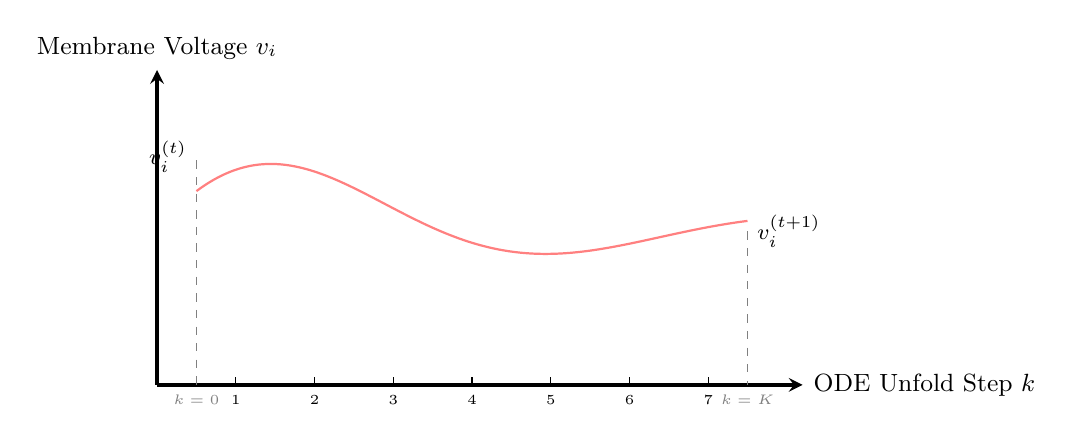
\begin{tikzpicture}[
        axis/.style={very thick, ->, >=stealth},
        voltage/.style={draw=red!50, thick, smooth},
        time/.style={font=\small},
        every node/.style={font=\small}
    ]

    % Axes
    \draw[axis] (0,0) -- (8.2,0) node[right] {ODE Unfold Step $k$};
    \draw[axis] (0,0) -- (0,4.0) node[above] {Membrane Voltage $v_i$};

    % Tick labels (k)
    \foreach \x in {1,2,...,7}
        \draw (\x,0) -- (\x,0.1) node[below=3pt] {\tiny $\x$};

    % Voltage trace (stylised)
    \draw[voltage, domain=0.5:7.5, samples=100] plot (\x, {2 + 1.2*sin(deg(0.9*\x))*exp(-0.25*\x)});

    % Annotate starting voltage
    \draw[dashed, gray] (0.5,2.85) -- (0.5,0) node[below] {\tiny $k=0$};
    \node at (0.5,2.9) [left, font=\footnotesize] {$v_i^{(t)}$};

    % Annotate final voltage
    \draw[dashed, gray] (7.5,1.95) -- (7.5,0) node[below] {\tiny $k=K$};
    \node at (7.5,1.95) [right, font=\footnotesize] {$v_i^{(t+1)}$};

    \end{tikzpicture}
    \caption{Illustrative internal membrane voltage trace across $K$ ODE unfolding steps for a single neuron. This entire graph represents the internal dynamics used to compute $v_i^{(t+1)}$ from $v_i^{(t)}$, in a single timestep.}
    \label{fig:lif_voltage_evolution}
\end{figure}

Unlike traditional RNNs or LSTMs, which update their hidden state in a single discrete operation per time step, Liquid Time-Constant neurons simulate fine-grained membrane voltage dynamics by performing multiple internal updates within each input timestep. This behaviour is governed by the discretised solution of the differential equations (see Equation~\ref{eq:v_update} and Equation~\ref{eq:v_update_denominator}).

At each unfolding step, the membrane potential is updated using a softplus-modulated combination of capacitive memory, leak current, and synaptic input currents. These updates reflect physical dynamics such as charging, leak, and synaptic integration, enabling the neuron to adaptively integrate information over sub-timestep resolution. The final membrane voltage $v_i^{(t+1)}$ is the result of this integration process and is passed forward in time.

This is different from gated memory in LSTMs, which uses learnable gates and affine transformations, or temporal convolutions in TCNs, which apply fixed receptive filters. Instead, the LTC neuron learns dynamic temporal behaviour through time constants and nonlinear integration, making it particularly suited to tasks that require fine temporal resolution and state-dependent transitions.

\vspace{1em}
\noindent \textbf{Implementation Details:}
\begin{itemize}
    \item \textbf{Learnable Parameters:} All biophysical constants (capacitance, leak conductance, reversal potentials, synaptic weights) are learnable, providing flexibility in dynamic behaviour.
    \item \textbf{Softplus Regularisation:} Weights and conductances are passed through \texttt{Softplus} to enforce positivity while allowing gradients to flow smoothly during training.
    \item \textbf{ODE Unfolding:} The number of internal solver steps is fixed (\texttt{ode\_unfolds} = 12) to balance numerical precision with computational cost.
    \item \textbf{Sparsity Masks:} Both recurrent and sensory activations are element-wise masked using the adjacency matrices from \texttt{RandomWiring}, enforcing fixed sparsity throughout training.
\end{itemize}

\noindent Below is the ODE solver implementation within the \texttt{LIFNeuronLayer} class:
\begin{lstlisting}[language=Python, caption={Simplified LTC neuron forward method}]
def ode_solver(self, inputs, state, elapsed_time):
    v_pre = state
    for _ in range(self.ode_unfolds):
        synaptic_input = compute_synaptic_activation(v_pre)
        numerator = self.cm * v_pre + self.gleak * self.vleak + synaptic_input
        denominator = self.cm + self.gleak + synaptic_conductance
        v_pre = numerator / (denominator + self.epsilon)
    return v_pre
\end{lstlisting}
This allows neurons to respond to both present input and also to their internal temporal dynamics, mimicking continuous-time memory traces observed in biological neurons.

\begin{figure}[H]
    \centering
    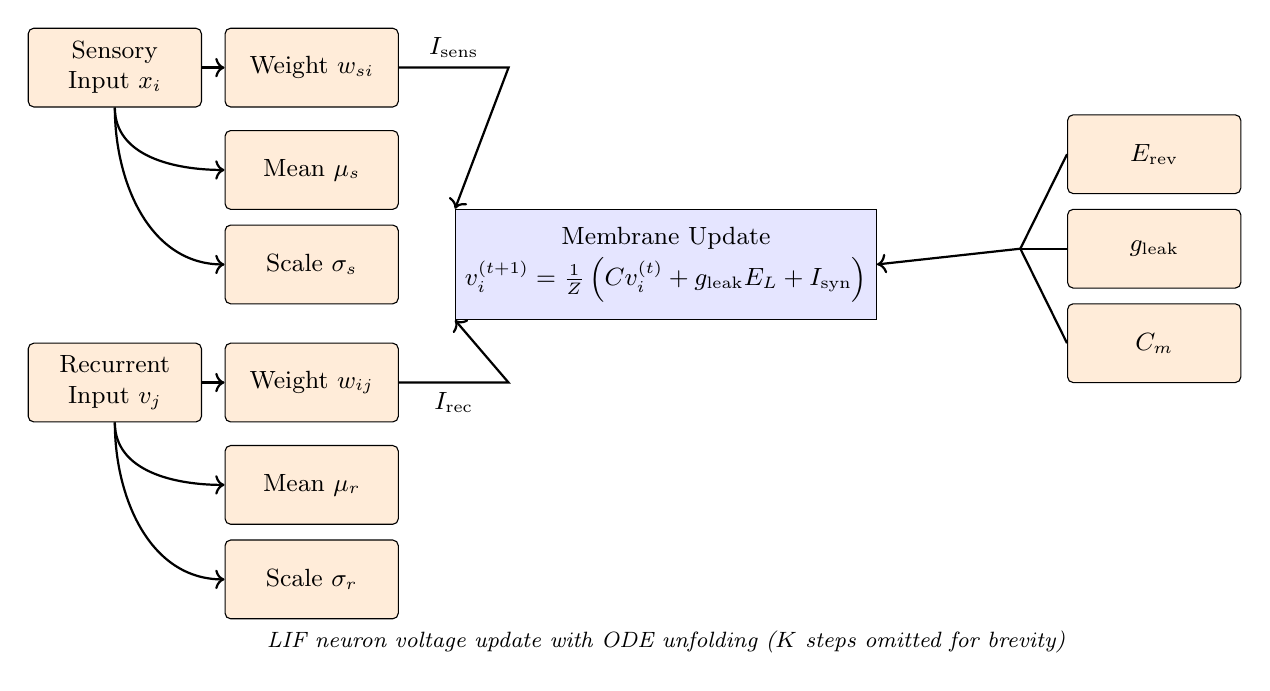
\begin{tikzpicture}[
        box/.style={draw, minimum height=1.4cm, minimum width=2.8cm, align=center, fill=blue!10},
        label/.style={font=\footnotesize\itshape},
        param/.style={draw, rounded corners=2pt, fill=orange!15, minimum height=1cm, minimum width=2.2cm, align=center},
        arrow/.style={->, thick},
        line/.style={-, thick},
        every node/.style={font=\small}
    ]
    
    % Sensory Input
    \node[param] (sens_input) at (-5, 3.5) {Sensory\\Input $x_i$};
    \node[param] (sens_w) at (-2.5, 3.5) {Weight $w_{si}$};
    \node[param] (sens_mu) at (-2.5, 2.2) {Mean $\mu_s$};
    \node[param] (sens_sigma) at (-2.5, 1.0) {Scale $\sigma_s$};
    \draw[arrow] (sens_input) -- (sens_w);
    \draw[arrow] (sens_input.south) to[out=270,in=180] (sens_mu.west);
    \draw[arrow] (sens_input.south) to[out=270,in=180] (sens_sigma.west);
    
    % Recurrent Input
    \node[param] (rec_input) at (-5, -0.5) {Recurrent\\Input $v_j$};
    \node[param] (rec_w) at (-2.5, -0.5) {Weight $w_{ij}$};
    \node[param] (rec_mu) at (-2.5, -1.8) {Mean $\mu_r$};
    \node[param] (rec_sigma) at (-2.5, -3.0) {Scale $\sigma_r$};
    \draw[arrow] (rec_input) -- (rec_w);
    \draw[arrow] (rec_input.south) to[out=270,in=180] (rec_mu.west);
    \draw[arrow] (rec_input.south) to[out=270,in=180] (rec_sigma.west);
    
    % Membrane Update Box
    \node[box] (voltage) at (2, 1.0) {Membrane Update\\[2pt] $v_i^{(t+1)} = \frac{1}{Z} \left(C v_i^{(t)} + g_\text{leak} E_L + I_{\text{syn}} \right)$};
    
    % Inputs into Membrane Box
    \draw[arrow] (sens_w.east) -- (0, 3.5) node[midway, above] {$I_{\text{sens}}$} -- (voltage.north west);
    \draw[arrow] (rec_w.east) -- (0, -0.5) node[midway, below] {$I_{\text{rec}}$} -- (voltage.south west);
    
    % Right-side parameters
    \node[param] (erev) at (8.2, 2.4) {$E_\text{rev}$};
    \node[param] (gleak) at (8.2, 1.2) {$g_\text{leak}$};
    \node[param] (cm) at (8.2, 0.0) {$C_m$};
    
    % Junction point
    \coordinate (rightjunction) at (6.5, 1.2);
    
    % Connect parameters to junction (no arrowheads)
    \draw[line] (erev.west) -- (rightjunction);
    \draw[line] (gleak.west) -- (rightjunction);
    \draw[line] (cm.west) -- (rightjunction);
    
    % Final arrow into voltage box
    \draw[arrow] (rightjunction) -- (voltage.east);
    
    % Caption
    \node[label] at (2, -3.8) {LIF neuron voltage update with ODE unfolding ($K$ steps omitted for brevity)};
    
    \end{tikzpicture}
    \caption{Internal structure of a single LIF neuron used in the Liquid Time-Constant Network. Inputs undergo non-linear transformations based on trainable $\mu$ and $\sigma$, and the resulting activations are integrated using biophysical parameters (leak conductance $g_\text{leak}$, membrane capacitance $C_m$, and reversal potentials $E_\text{rev}$).}
    \label{fig:lif_neuron_detailed}
\end{figure}


\section{Network Architecture}
The full LNN is constructed by embedding the LTC neuron layer inside a recurrent wrapper, implemented as a custom \texttt{LTCRNN} module. This wrapper sequentially passes each time step of the input through the same \texttt{LIFNeuronLayer}, maintaining a hidden state that evolves over time. The resulting structure can be viewed as a biologically grounded alternative to traditional RNN cells.

The architecture accepts an input tensor of shape $(B, T, d_{\text{in}})$, where $B$ is the batch size, $T$ is the sequence length, and $d_{\text{in}}$ is the input dimension (two in this case, corresponding to 2D spatial coordinates). For each time step $t$, the neuron layer receives the $t$-th slice of the sequence and updates the hidden state, generating a predicted output of shape $(B, T, d_{\text{out}})$.

\subsection*{Design Considerations}
While designing the LTCRNN architecture, there were several key design decisions made. The hidden state dimensionality (i.e. number of LTC neurons) defined the model capacity; lower values reduce overfitting risk and improve computational efficiency at the cost of limited expressiveness. In addition, the voltage traces themselves are treated as predictions instead of applying a separate output layer. This means membrane state is directly used as a continuous output signal. To maximise efficiency (and GPU parallelism) of tensor operations during training/inference, all sequences are processed in batch-major form (following PyTorch convention).

\noindent Below is a simplified version of this architecture:
\begin{lstlisting}[language=Python, caption={Structure of the LTCRNN module}]
class LTCRNN(nn.Module):
    def __init__(self, wiring, input_dim, hidden_dim, output_dim):
        self.cell = LIFNeuronLayer(wiring)
        ...
        
    def forward(self, inputs):
        batch_size, seq_len, _ = inputs.size()
        states = torch.zeros(batch_size, self.hidden_dim)
        outputs = []
        for t in range(seq_len):
            out, states = self.cell(inputs[:, t, :], states)
            outputs.append(out)
        return torch.stack(outputs, dim=1)
\end{lstlisting}

The design maintains a clear distinction between the continuous-time neuronal dynamics and the sequence-level integration logic. Thus, it is both modular and biologically interpretable, and compatible with standardised modern deep learning tools.

\begin{figure}[H]
    \centering
    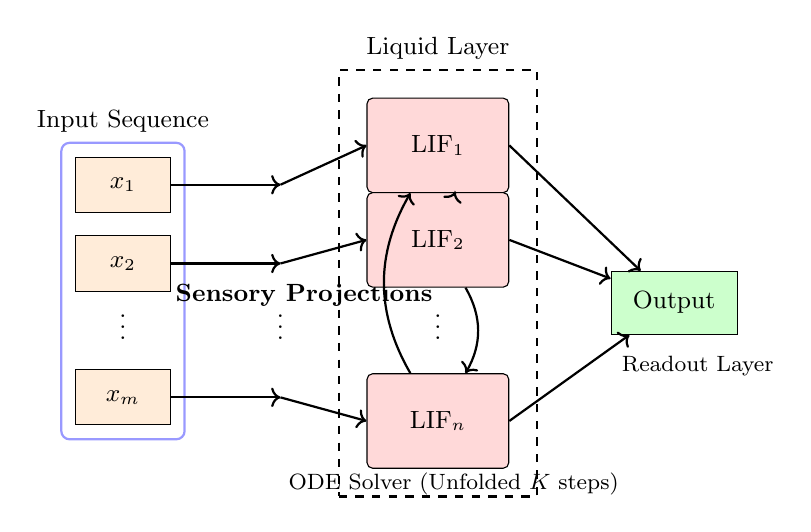
\begin{tikzpicture}[
        neuron/.style={circle, draw=black, fill=blue!15, minimum size=1.2cm},
        lif/.style={rectangle, draw=black, rounded corners=2pt, fill=red!15, minimum height=1.2cm, minimum width=1.8cm},
        input/.style={draw=black, fill=orange!15, minimum width=1.2cm, minimum height=0.7cm, text centered},
        output/.style={draw=black, fill=green!20, minimum width=1.6cm, minimum height=0.8cm, text centered},
        arrow/.style={->, thick},
        every node/.style={font=\small}
    ]

    % Input block
    \node[input] (input1) at (0,1.5) {$x_1$};
    \node[input] (input2) at (0,0.5) {$x_2$};
    \node at (0,-0.2) {$\vdots$};
    \node[input] (inputm) at (0,-1.2) {$x_m$};

    \node[draw=blue!40, thick, rounded corners=3pt, fit=(input1)(input2)(inputm), inner sep=5pt, label=above:Input Sequence] (inputbox) {};

    % Sensory Projection
    \node at (2.3, 0.1) {\textbf{Sensory Projections}};
    \draw[arrow] (input1) -- (2,1.5);
    \draw[arrow] (input2) -- (2,0.5);
    \draw[arrow] (inputm) -- (2,-1.2);
    \node at (2,-0.2) {$\vdots$};

    % LIF Neuron Layer (Liquid Layer)
    \node[lif] (lif1) at (4,2.0) {LIF$_1$};
    \node[lif] (lif2) at (4,0.8) {LIF$_2$};
    \node at (4,-0.2) {$\vdots$};
    \node[lif] (lifn) at (4,-1.5) {LIF$_n$};
    
    \node[draw=black, thick, dashed, fit=(lif1)(lif2)(lifn), inner sep=10pt, label=above:Liquid Layer] (liquidbox) {};

    % Internal recurrent wiring (sparse)
    \draw[arrow, bend left=20] (lif1) to (lif2);
    \draw[arrow, bend left=30] (lif2) to (lifn);
    \draw[arrow, bend left=30] (lifn) to (lif1);

    % Sensory to Liquid
    \draw[arrow] (2,1.5) -- (lif1.west);
    \draw[arrow] (2,0.5) -- (lif2.west);
    \draw[arrow] (2,-1.2) -- (lifn.west);

    % Output Projection (Readout)
    \node[output] (out) at (7,0) {Output};

    \draw[arrow] (lif1.east) -- (out);
    \draw[arrow] (lif2.east) -- (out);
    \draw[arrow] (lifn.east) -- (out);

    % Labels
    \node at (4.2,-2.3) {\footnotesize ODE Solver (Unfolded $K$ steps)};
    \node at (7.3,-0.8) {\footnotesize Readout Layer};

    \end{tikzpicture}
    \caption{Architecture of the Liquid Time-Constant Network (LNN). Inputs project through learned sensory filters to a sparsely recurrent Liquid Layer of LIF neurons. Dynamics are integrated using an internal ODE solver with unfolding. Final outputs are read from a low-dimensional projection.}
    \label{fig:lnn_architecture}
\end{figure}


\section{Training Configuration (and dataset)}
The LNN was trained on a synthetic 2D spiral trajectory dataset, chosen for its smooth temporal structure and nonlinearity. Each data point consists of an $(x, y)$ coordinate, and the model's aim is to predict the next point in the sequence (given a fixed-length input window). The 'sequential' nature of the task makes it well-suited for testing temporal memory and continuous dynamics.

The synthetically-generated dataset ensured control over noise and resolution, which allowed clearer attribution of error sources to model limitations rather than data irregularities.

A supervised learning approach was used; inputs and targets were created by shifting a sliding window of length $T = 3$ over the full spiral. The small sequence length was chosen to reduce training complexity while still allowing temporal dependencies to be captured. Each input sequence of three time steps was paired with the corresponding next three steps as the target output.

The dataset was split into training and validation sets, with the training set containing 80\% of the data and the validation set containing 20\%. This split was randomised to ensure that the model generalised well to unseen data.

\subsubsection*{Data Preprocessing}
\begin{itemize}
    \item All inputs were standardised using the training set mean and standard deviation.
    \item Targets were normalised in the same way to preserve scale consistency.
    \item The spiral dataset was generated programmatically with adjustable number of points and turns.
\end{itemize}

subsubsection*{Training Parameters}
Mean Squared Error (\texttt{nn.MSELoss()}) was used to penalise deviations from the ground truth trajectory. Adam was chosen as the optimiser due to its fast convergence and robustness to parameter scaling, with a learning rate of 0.005. The model was trained for 2000 epochs, with periodic visual evaluation every 100 epochs. Input sequences were split into overlapping windows and grouped into batches of size 32, allowing efficient GPU utilisation while preserving temporal continuity. A random 80/20 train-validation split was applied, with shuffling to prevent memorisation of input order.

Below is the training process implementation:
\begin{lstlisting}[language=Python, caption={Simplified training loop for the LNN}]
for epoch in range(num_epochs):
    lnn_model.train()
    total_loss = 0
    for x_batch, y_batch in zip(input_batches, target_batches):
        optimizer.zero_grad()
        outputs = lnn_model(x_batch)
        loss = criterion(outputs, y_batch)
        loss.backward()
        optimizer.step()
        total_loss += loss.item()
\end{lstlisting}

The training loop includes evaluation checkpoints where predicted trajectories are plotted and compared to ground truth. These visualisations provided insights into convergence behaviour, beyond scalar loss values.

\section{Training Behaviour}
Throughout training, model performance was monitored both quantitatively (via validation loss) and qualitatively (through trajectory plots), every 100 epochs.

\noindent The main trends observed during training were:
\begin{itemize}
    \item Loss decreased steadily in early epochs, with diminishing returns as training progressed.
    \item In some cases, small fluctuations in validation loss were observed, likely due to the non-convexity of the parameter landscape and the biological variability induced by random wiring.
    \item Visual predictions of the trajectory showed clear improvement over time. Early predictions were coarse approximations, while later epochs gave smoother and more accurate predictions.
\end{itemize}

\subsection*{Trajectory Loss Curves}
To evaluate the model's learning progress and generalisation, we record the full-sequence mean squared error (MSE) first on the entire spiral sequence (which contains the training datapoints and the held-out validation datapoints), and then on a separate unseen evaluation spiral, at each epoch. Rather than separately plotting training and validation loss — which are contiguous segments of the same spiral trajectory, they are treated as a single sequence. This is because temporal continuity is essential in modelling dynamical systems. This avoids misleading interpretations that might arise from artificial segmentation of a naturally evolving system.

The following plots illustrates training and validation behaviour over time (the second is zoomed to highlight differences between the training/validation spiral and evaluation spiral):

\begin{figure}[H]
    \centering
    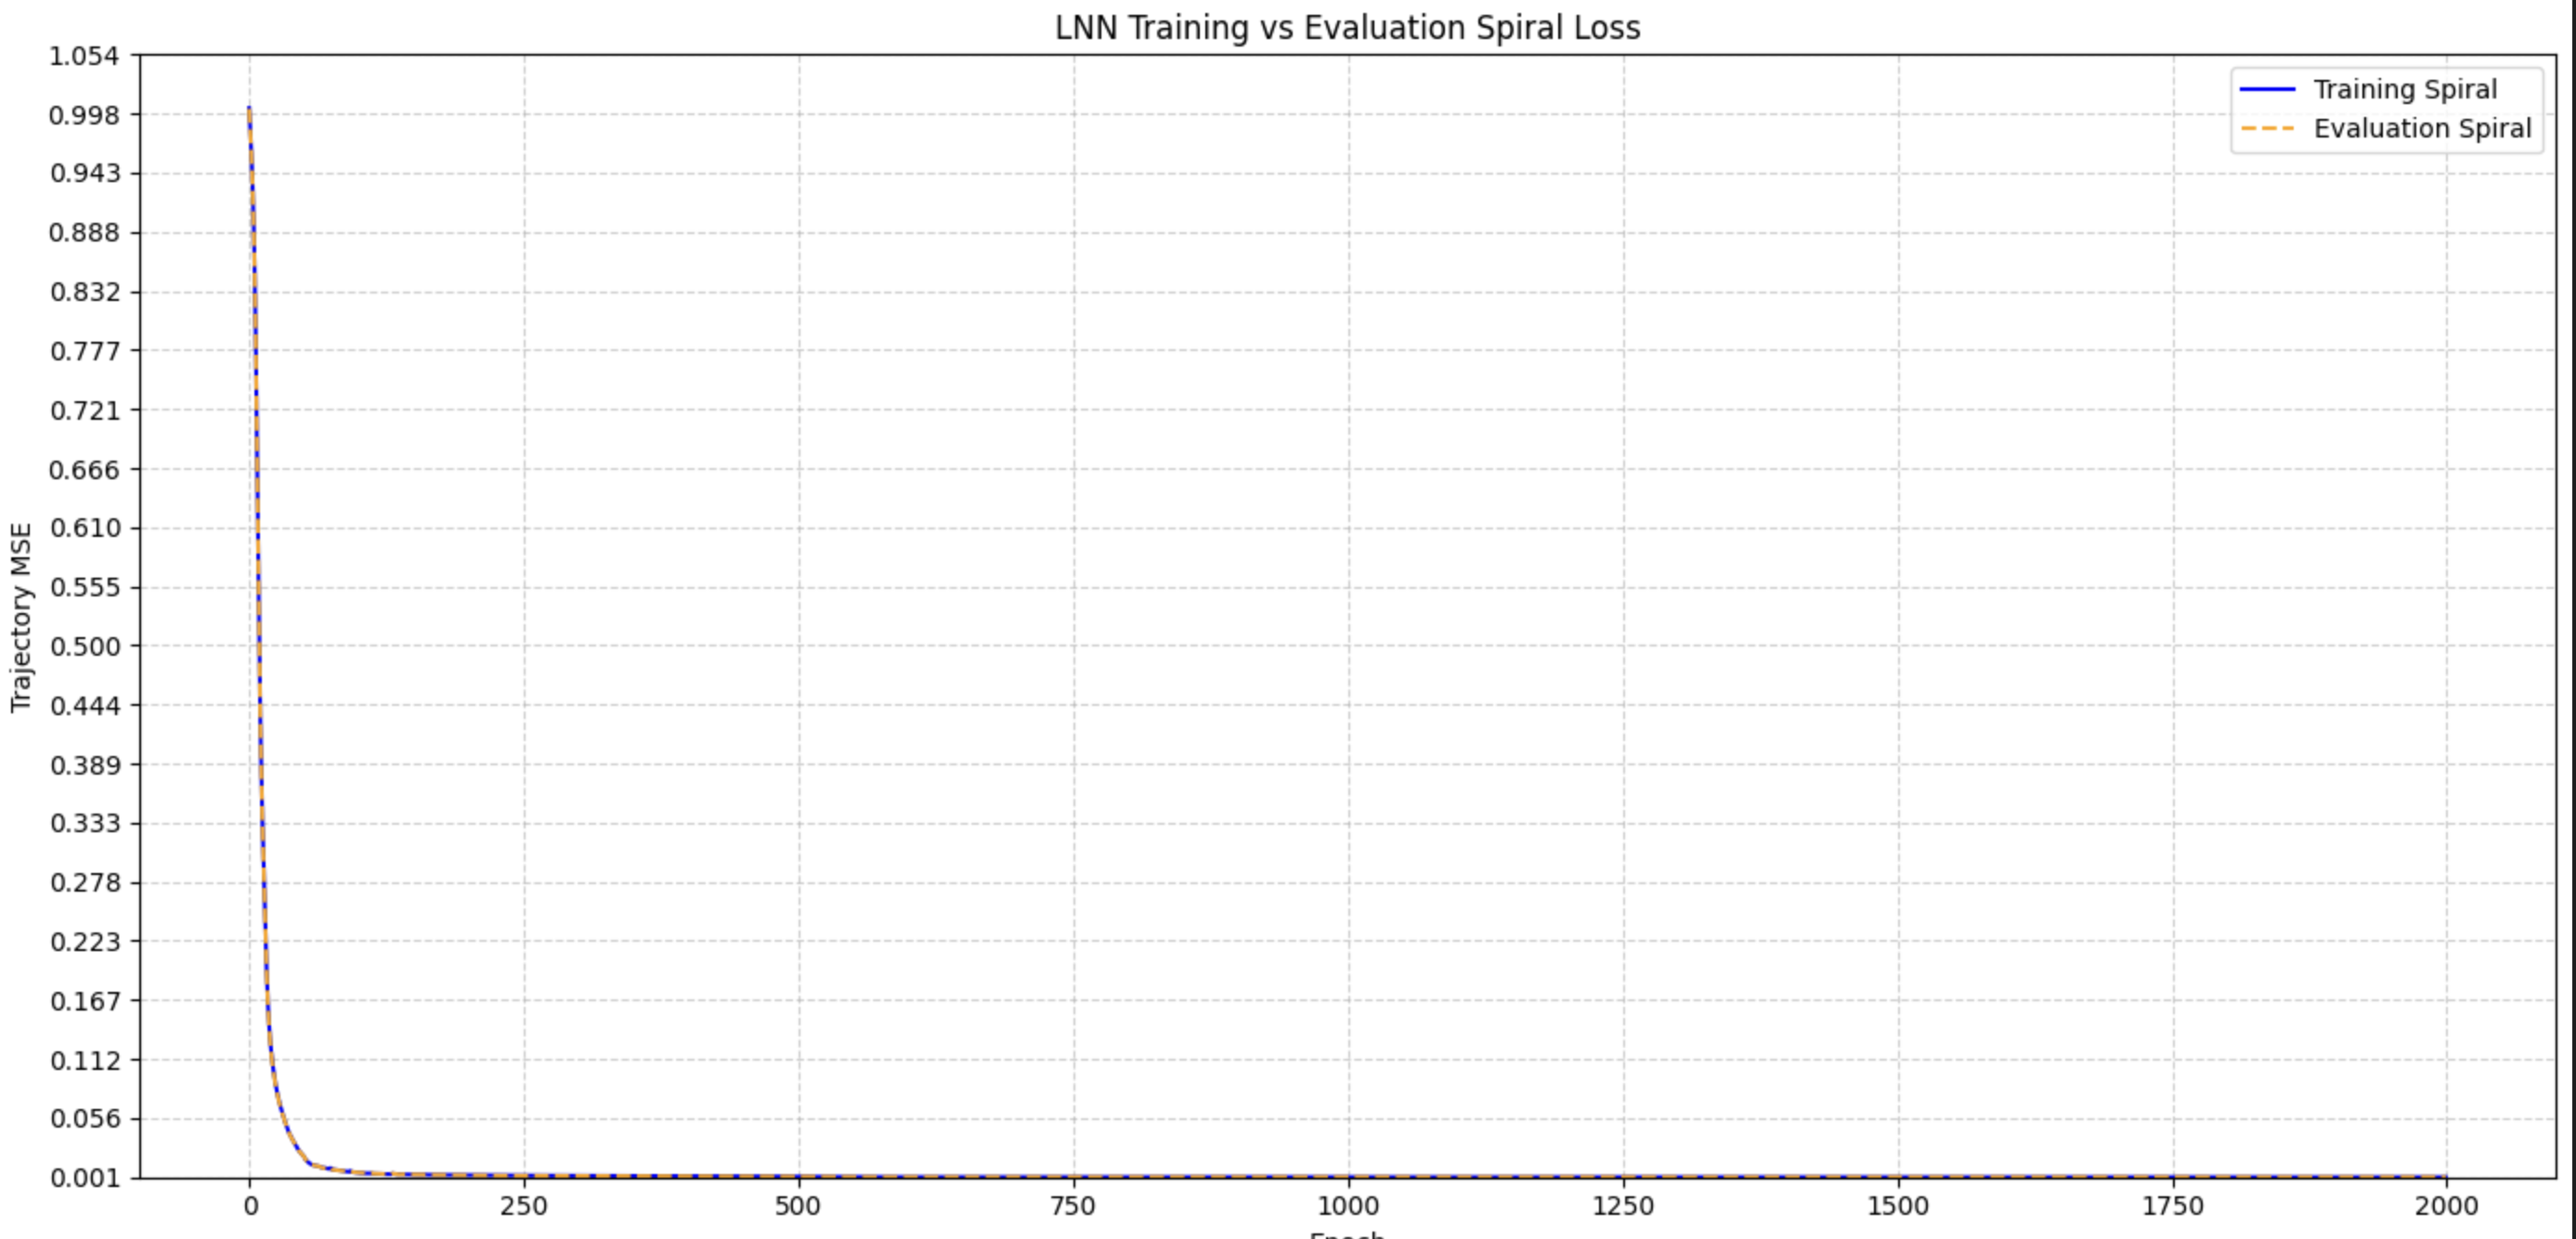
\includegraphics[width=0.8\linewidth]{img/lnn_loss_curve.png}
    \caption{Training and validation loss over epochs.}
    \label{fig:lnn_loss}
\end{figure}

\begin{figure}[H]
    \centering
    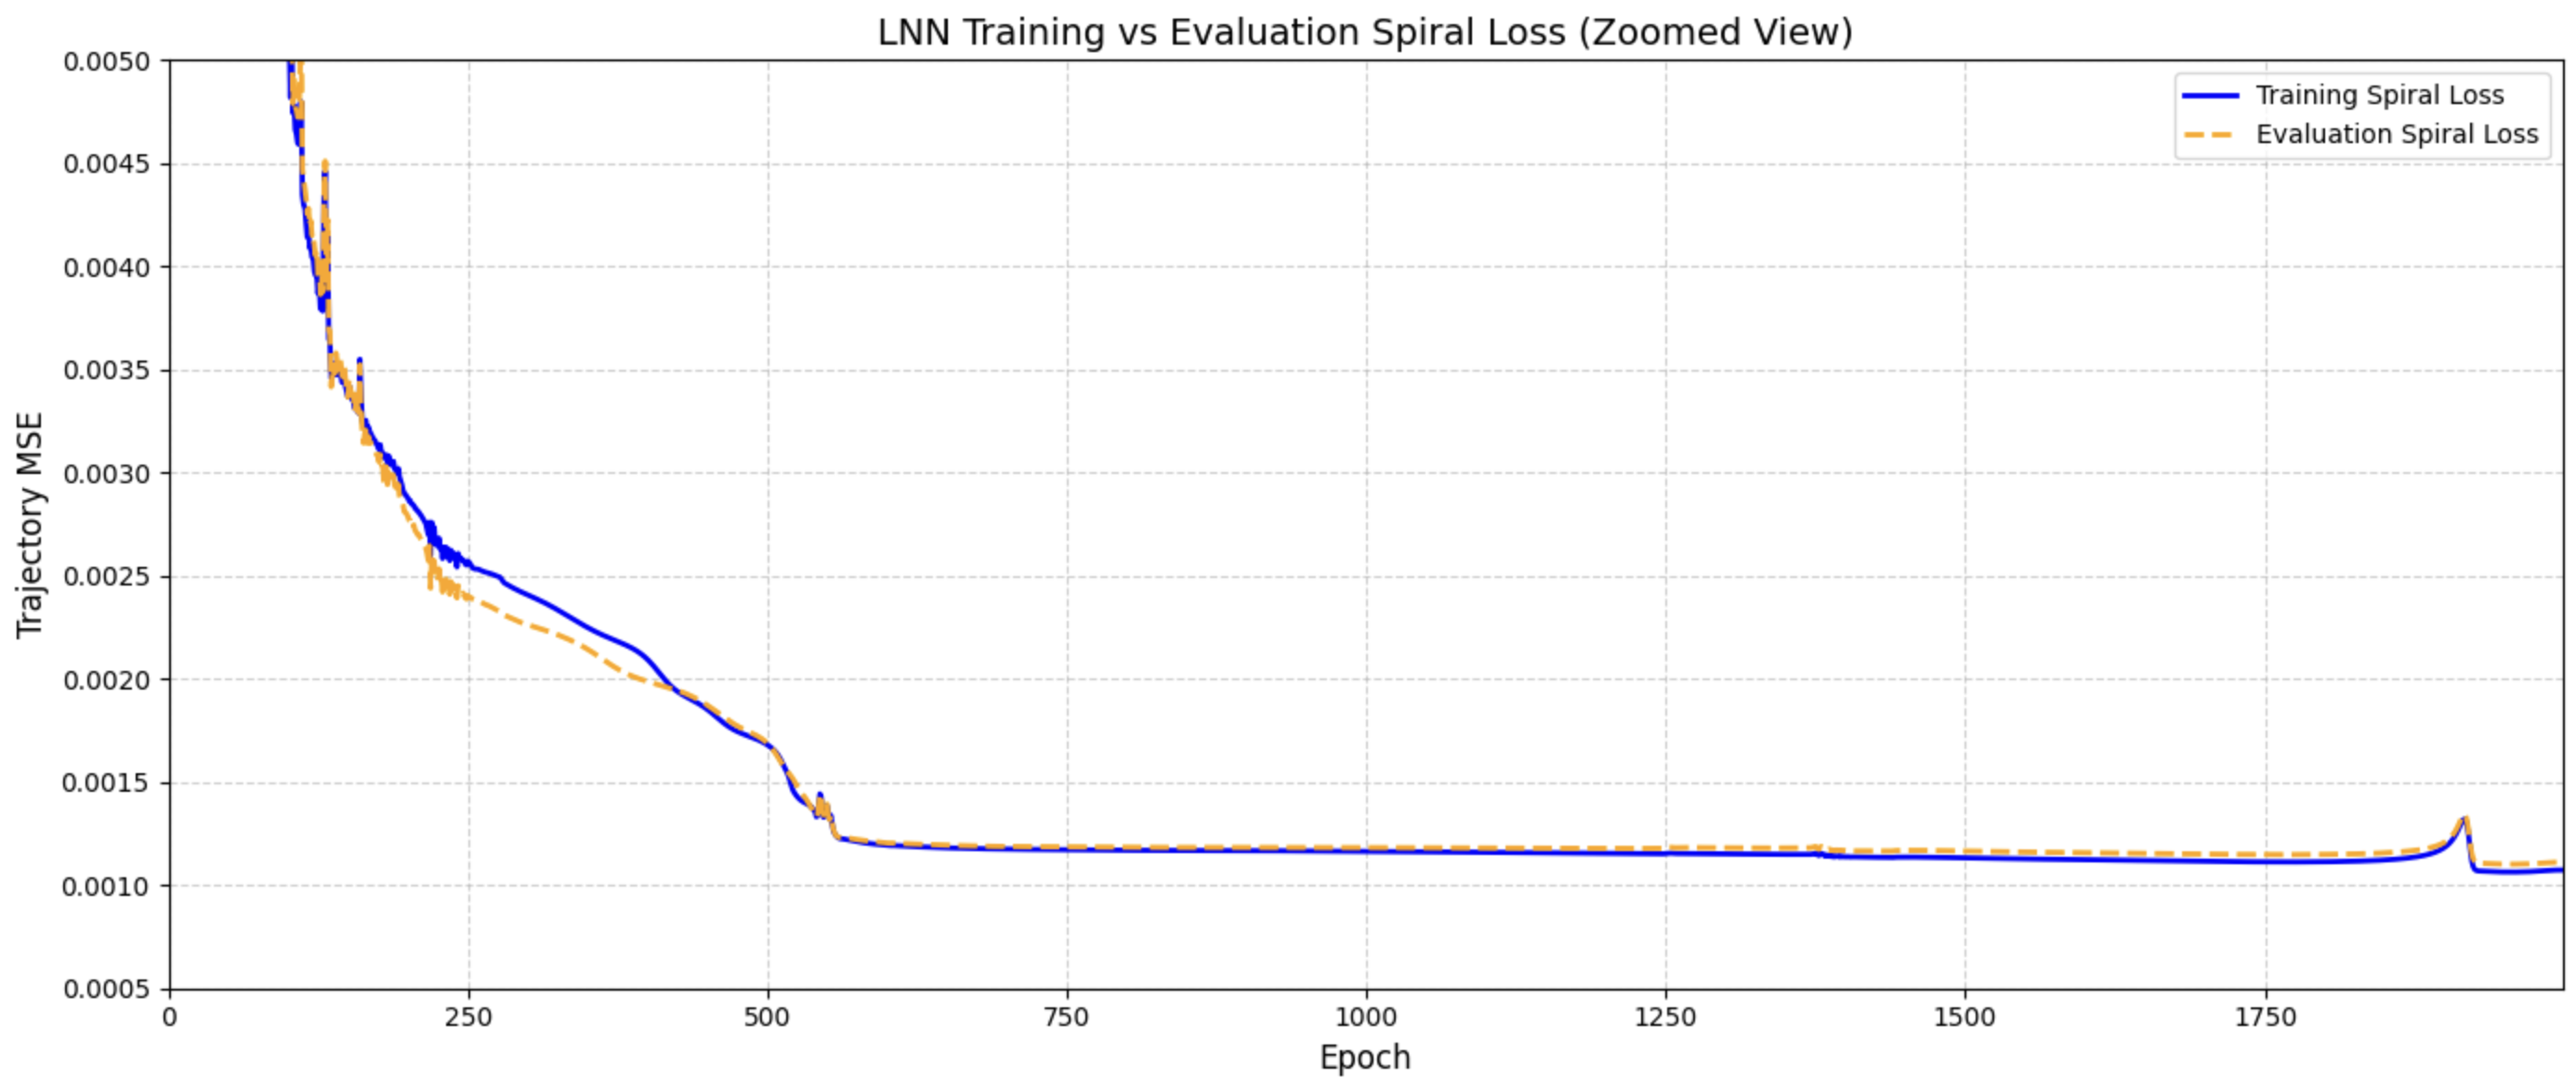
\includegraphics[width=0.8\linewidth]{img/lnn_loss_curve_zoomed.png}
    \caption{Training and validation loss over epochs (zoomed).}
    \label{fig:lnn_loss_zoomed}
\end{figure}

Early in training, both curves decrease rapidly, suggesting that the model learns the underlying structure efficiently. As training proceeds, the two curves converge, with the evaluation spiral maintaining a slightly higher loss, indicating some generalisation gap but also demonstrating stable extrapolation beyond the training path. Importantly, neither curve exhibits significant divergence or overfitting behaviour, which supports the robustness and consistency of the trained model.

\subsection*{Qualitative Evaluation}
Visually, the predicted path over time showed that the LNN was able to maintain smooth curvature and approximate the rotational dynamics of the spiral without overshooting or excessive lag. This was true even on validation data not seen during training. 

\begin{figure}[H]
    \centering
    \begin{subfigure}[b]{0.45\linewidth}
        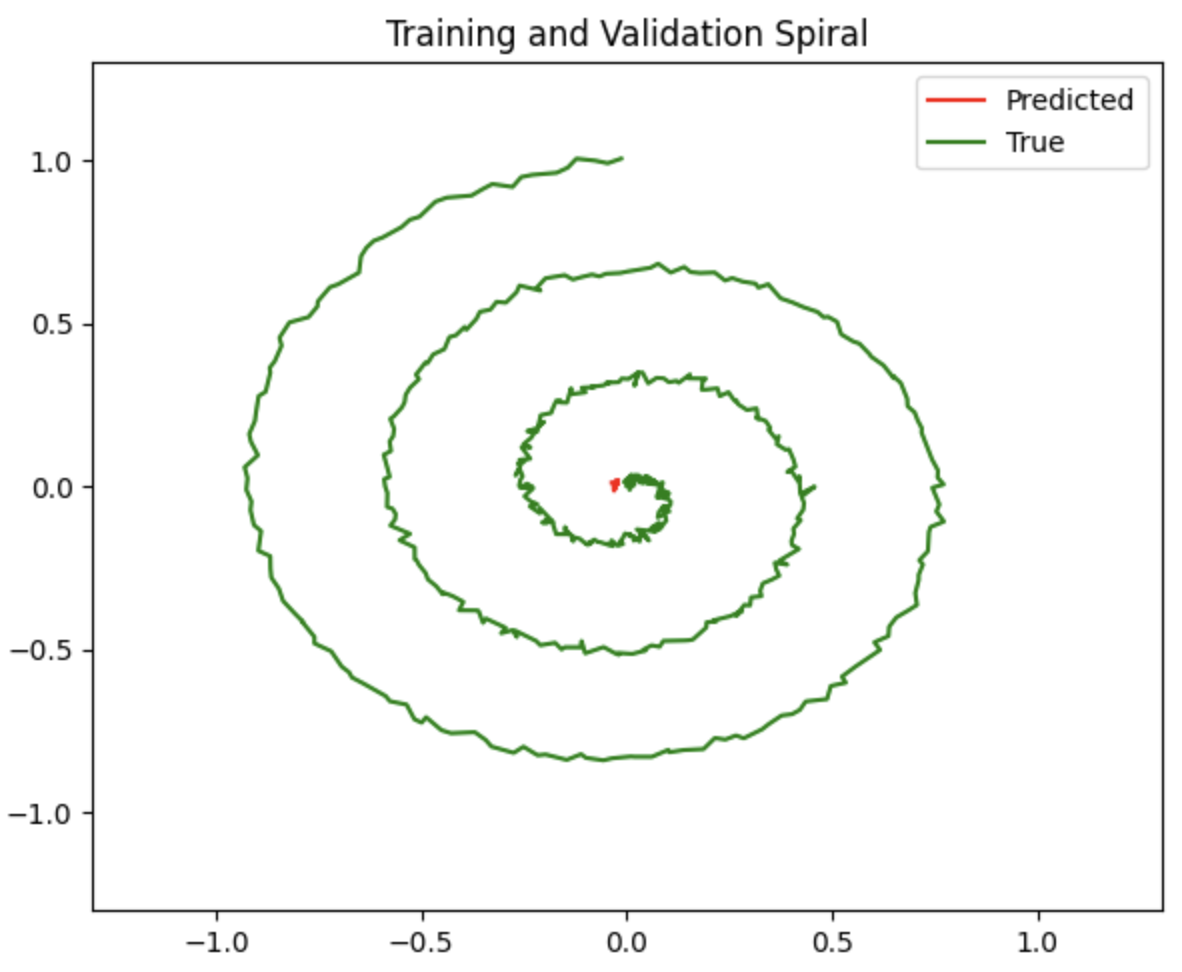
\includegraphics[width=\linewidth]{img/lnn_training_validation_spiral_epoch_1.png}
        \caption{Epoch 1}
        \label{fig:lnn_training_validation_spiral_epoch_1}
    \end{subfigure}
    \hfill
    \begin{subfigure}[b]{0.45\linewidth}
        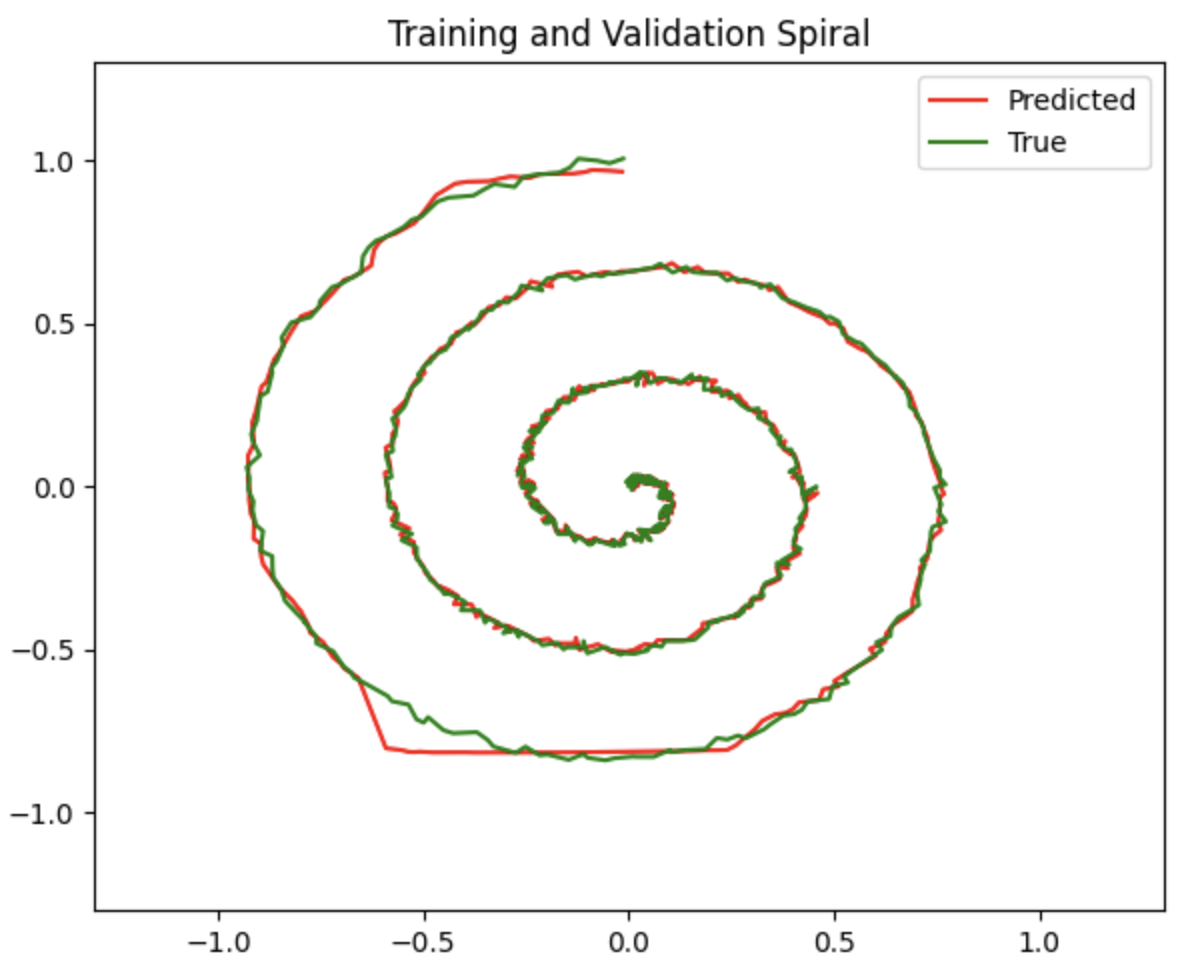
\includegraphics[width=\linewidth]{img/lnn_training_validation_spiral_epoch_400.png}
        \caption{Epoch 400}
        \label{fig:lnn_training_validation_spiral_epoch_400}
    \end{subfigure}
    \vskip\baselineskip
    \begin{subfigure}[b]{0.45\linewidth}
        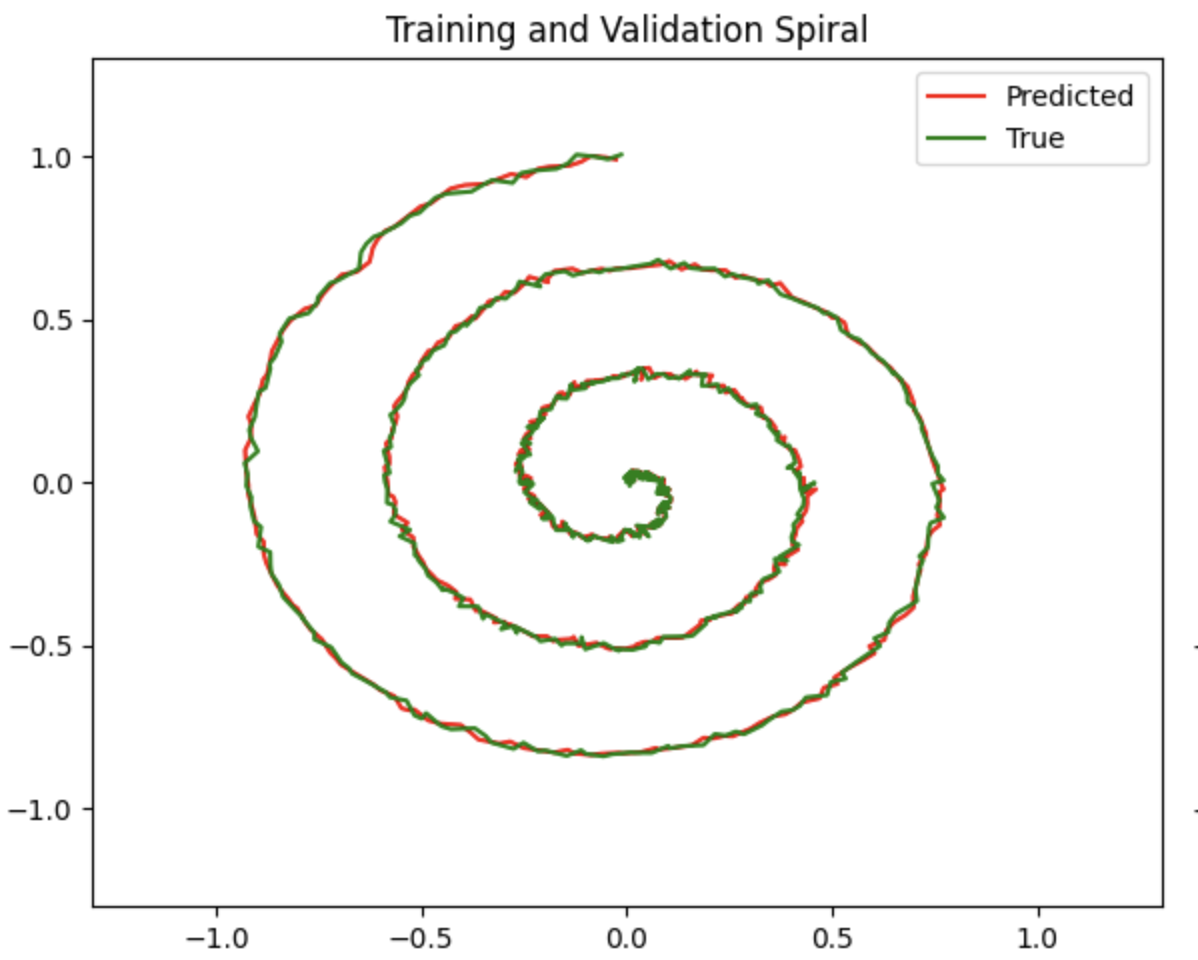
\includegraphics[width=\linewidth]{img/lnn_training_validation_spiral_epoch_2000.png}
        \caption{Epoch 2000}
        \label{fig:lnn_training_validation_spiral_epoch_2000}
    \end{subfigure}
    \caption{LLN predicted vs true spiral trajectories across training: early, mid, and final epochs (denormalised training and validation spiral)}
    \label{fig:lnn_spiral_progression_grid}
\end{figure}

\subsection*{Observed Patterns Across Training Runs}
The number of internal steps in the membrane integration process (\textbf{ODE unfolding depth}) contributed significantly to trajectory stability. Deeper unfolding improved smoothness, but with diminishing returns. The architectures' fixed wiring helped constrain overfitting and contributed to better generalisation than a fully connected architecture. Notably, runs with different initialisations showed \textbf{performance variations} in loss curves and convergence speed, indicating sensitivity to initial wiring or parameter seeds.

Despite simpler architectures having shorter training times (e.g. LSTMs), LLN's had superior interprebility and stability in capturing the underlying continuous structure of the problem.

Although trained on fixed-length input windows, models were evaluated on full-sequence inference without autoregressive rollouts. This mismatch is empirically validated to yield stable and accurate predictions on smooth trajectories.
\chapter{Comparative Models}

\section{Introduction to Baseline Models}

To provide context for the robustness and verification of the Liquid Neural Network (LNN), we benchmark its performance against three established neural architectures: the Temporal Convolutional Network (TCN), the Long Short-Term Memory (LSTM) network, and the Transformer model. All models are trained on the same trajectory prediction task, using identical datasets, normalisation, loss functions, and training schedules as the LNN.

The selection of these baselines is motivated by their contrasting inductive biases and proven success in modelling sequential data. The LSTM is a recurrent architecture that introduces gating mechanisms and persistent internal states, enabling it to model long-range temporal dependencies through iterative state updates. The TCN, however, uses on dilated causal convolutions and fixed temporal receptive fields, making it structurally different from recurrent networks and well-suited for parallel computation. The transformer model is an attention-based architecture, which eliminates recurrence altogether, and dynamically weight input positions using self-attention mechanisms. It applies positional encodings to retain order information.

Each model is carefully designed and trained to have similar loss and accuracy (details of which can be found in evaluation \ref{chap:evaluation}). This allows for fair comparison of robustness.

By evaluating the behaviour of these models under clean and adversarial conditions, we aim to identify both their predictive accuracy, and their robustness, sensitivity to perturbation, and qualitative output characteristics. These insights provide context for assessing the LNN in the following aspects:

\begin{itemize}
    \item \textbf{Temporal memory:} How effectively each model retains and processes sequential dependencies
    \item \textbf{Structural robustness:} The influence of architectural constraints on noise sensitivity
    \item \textbf{Gradient stability:} The relationship between loss geometry and adversarial vulnerability
\end{itemize}


\section{Temporal Convolutional Network (TCN)}

\subsection*{Overview and Motivation}
The TCN is a fully convolutional architecture designed for sequential data. Unlike RNN-based models, which process inputs recursively and maintain an internal hidden state, TCNs rely on 1D convolutions applied over the temporal axis. This allows for parallel computation and more stable gradients, particularly for long sequences.

TCN's use \textbf{dilated convolutions}, which expand the receptive field exponentially with depth while preserving causality. This makes them highly effective at modelling long-range dependencies without the vanishing gradient issues that often affect RNNs.

\subsection*{Theoretical Background}
For a 1D input sequence $x \in \mathbb{R}^{T \times d}$, a dilated convolution with kernel $k$ and dilation factor $d$ is defined as:
\[
(y *_{d} k)(t) = \sum_{i=0}^{k-1} k(i) \cdot x(t - d \cdot i)
\]
This structure allows the model to observe wider contexts with fewer parameters and layers.

In practice, the TCN is constructed using \textbf{residual blocks} with stacked dilated convolutions, dropout, and skip connections to stabilise training. Zero-padding is used to ensure output length matches input length.

\subsection*{Model Architecture}
The implemented TCN consists of 3 residual blocks, each with: two dilated 1D convolutional layers with kernel size 3, ReLU activations and dropout regularisation, and optional 1x1 convolutions for matching input-output dimensions. Each residual block has a dilation rate of 1, 2, and 4 respectively (exponentially increasing dilation).

An output convolution maps the final hidden representation to the desired 2D coordinate space.

Below is a simplified example of the TCN model implementation:

\begin{lstlisting}[language=Python, caption={Simplified TCN architecture}]
class ResidualBlock(nn.Module):
    def __init__(self, in_channels, out_channels, kernel_size, dilation, dropout):
        ...
        self.conv1 = nn.Conv1d(..., dilation=dilation)
        self.conv2 = nn.Conv1d(..., dilation=dilation)

class TCN(nn.Module):
    def __init__(self, input_dim=2, hidden_channels=128, ...):
        self.tcn = nn.Sequential(*residual_blocks)
        self.output_layer = nn.Conv1d(hidden_channels, output_dim, 1)
\end{lstlisting}

\begin{figure}[H]
    \centering
    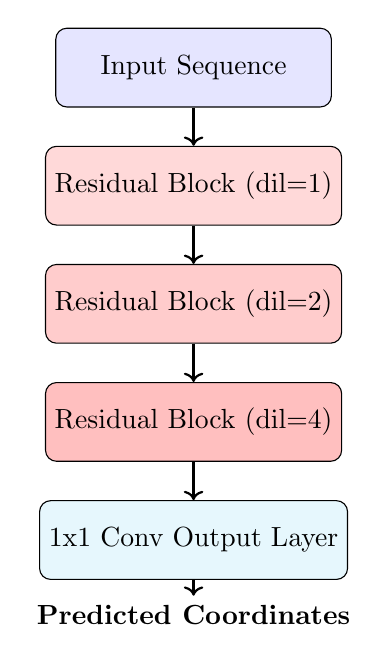
\begin{tikzpicture}[scale=1, every node/.style={transform shape}]

        % Input
        \node[draw, rounded corners, minimum width=3.5cm, minimum height=1cm, fill=blue!10] (input) at (0, 0) {Input Sequence};

        % Residual Block 1
        \node[draw, rounded corners, minimum width=3.5cm, minimum height=1cm, fill=red!15] (res1) at (0, -1.5) {Residual Block (dil=1)};
        \draw[->, thick] (input) -- (res1);

        % Residual Block 2
        \node[draw, rounded corners, minimum width=3.5cm, minimum height=1cm, fill=red!20] (res2) at (0, -3.0) {Residual Block (dil=2)};
        \draw[->, thick] (res1) -- (res2);

        % Residual Block 3
        \node[draw, rounded corners, minimum width=3.5cm, minimum height=1cm, fill=red!25] (res3) at (0, -4.5) {Residual Block (dil=4)};
        \draw[->, thick] (res2) -- (res3);

        % Output Conv
        \node[draw, rounded corners, minimum width=3.5cm, minimum height=1cm, fill=cyan!10] (out) at (0, -6.0) {1x1 Conv Output Layer};
        \draw[->, thick] (res3) -- (out);

        % Output
        \node[below=0.2cm of out] (final) {\textbf{Predicted Coordinates}};
        \draw[->, thick] (out) -- (final);

    \end{tikzpicture}
    \caption{Temporal Convolutional Network (TCN) architecture}
    \label{fig:tcn_architecture}
\end{figure}

\begin{figure}[H]
    \centering
    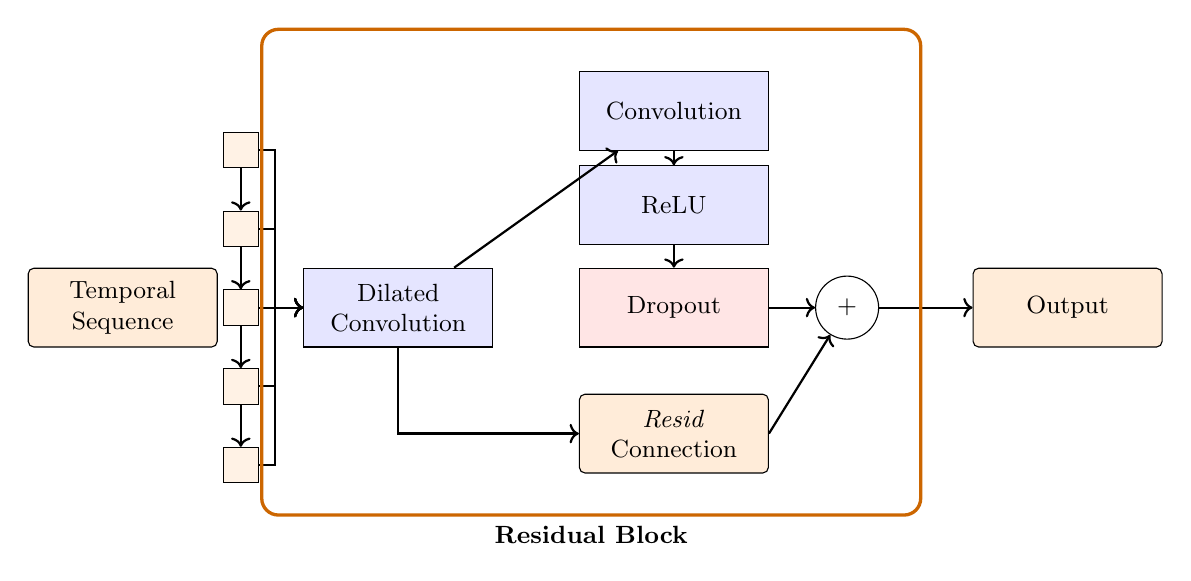
\begin{tikzpicture}[
        box/.style={draw, rounded corners=2pt, minimum width=2.4cm, minimum height=1cm, align=center, fill=orange!15},
        conv/.style={draw, minimum width=2.4cm, minimum height=1cm, align=center, fill=blue!10},
        dropout/.style={draw, minimum width=2.4cm, minimum height=1cm, align=center, fill=red!10},
        every node/.style={font=\small},
        arrow/.style={->, thick}
    ]

    % Input sequence label
    \node[box] (seq) at (-5, 0) {Temporal\\Sequence};

    % Input nodes (spaced vertically)
    \node[draw, fill=orange!10, minimum size=0.45cm] (in1) at (-3.5, 2.0) {};
    \node[draw, fill=orange!10, minimum size=0.45cm] (in2) at (-3.5, 1.0) {};
    \node[draw, fill=orange!10, minimum size=0.45cm] (in3) at (-3.5, 0) {};
    \node[draw, fill=orange!10, minimum size=0.45cm] (in4) at (-3.5, -1.0) {};
    \node[draw, fill=orange!10, minimum size=0.45cm] (in5) at (-3.5, -2.0) {};

    % Arrow from Temporal Sequence (avoid overlap)
    % \draw[arrow] (seq.east) -- ++(0.4, 0) -- ++(0, -2.4) -| (in3.west);

    % Arrows between input nodes
    \foreach \i/\j in {in1/in2, in2/in3, in3/in4, in4/in5}
        \draw[->, thick] (\i) -- (\j);

    % Dilated conv
    \node[conv] (dilated) at (-1.5, 0) {Dilated\\Convolution};
    \foreach \n in {in1,in2,in3,in4,in5}
        \draw[arrow] (\n.east) -- ++(0.2, 0) |- (dilated.west);

    % Inside residual block
    \node[conv] (conv1) at (2, 2.5) {Convolution};
    \node[conv] (relu)  at (2, 1.3) {ReLU};
    \node[dropout] (drop) at (2, 0) {Dropout};
    \node[draw, minimum size=0.8cm, circle, fill=white] (add) at (4.2, 0) {$+$};
    \node[box] (resid) at (2, -1.6) {\textit{Resid}\\Connection};

    % Arrows (main path)
    \draw[arrow] (dilated) -- (conv1);
    \draw[arrow] (conv1) -- (relu);
    \draw[arrow] (relu) -- (drop);
    \draw[arrow] (drop) -- (add);

    % Residual connection
    \draw[arrow] (dilated.south) |- (resid);
    \draw[arrow] (resid.east) -- (add);

    % Output
    \node[box] (output) at (7.0, 0) {Output};
    \draw[arrow] (add) -- (output.west);

    % Residual block container
    \node[draw=orange!80!black, very thick, rounded corners=6pt,
          fit=(dilated)(conv1)(drop)(resid)(add), inner sep=15pt,
          label=below:{\textbf{Residual Block}}] (block) {};

    \end{tikzpicture}
    \caption{Structure of a TCN Residual Block. Each convolution uses dilation to increase receptive field, while residual skip connections and dropout stabilise training.}
    \label{fig:tcn_residual_block}
\end{figure}

\subsection*{Training Configuration}
The TCN was trained on the same spiral dataset as the LNN, with identical batch size, learning rate, loss function (Smooth L1), and normalisation pipeline. The model was optimised using Adam and a learning rate scheduler that halved the rate every 500 steps.

\subsection*{Performance and Behaviour}
The TCN demonstrated strong performance on the trajectory prediction task, converging more quickly than the LNN and producing smooth outputs even with a small receptive field. The use of dilated convolutions allowed the model to predict coordinated curvature without explicitly tracking hidden state over time.

\begin{figure}[H]
    \centering
    \begin{subfigure}[b]{0.45\linewidth}
        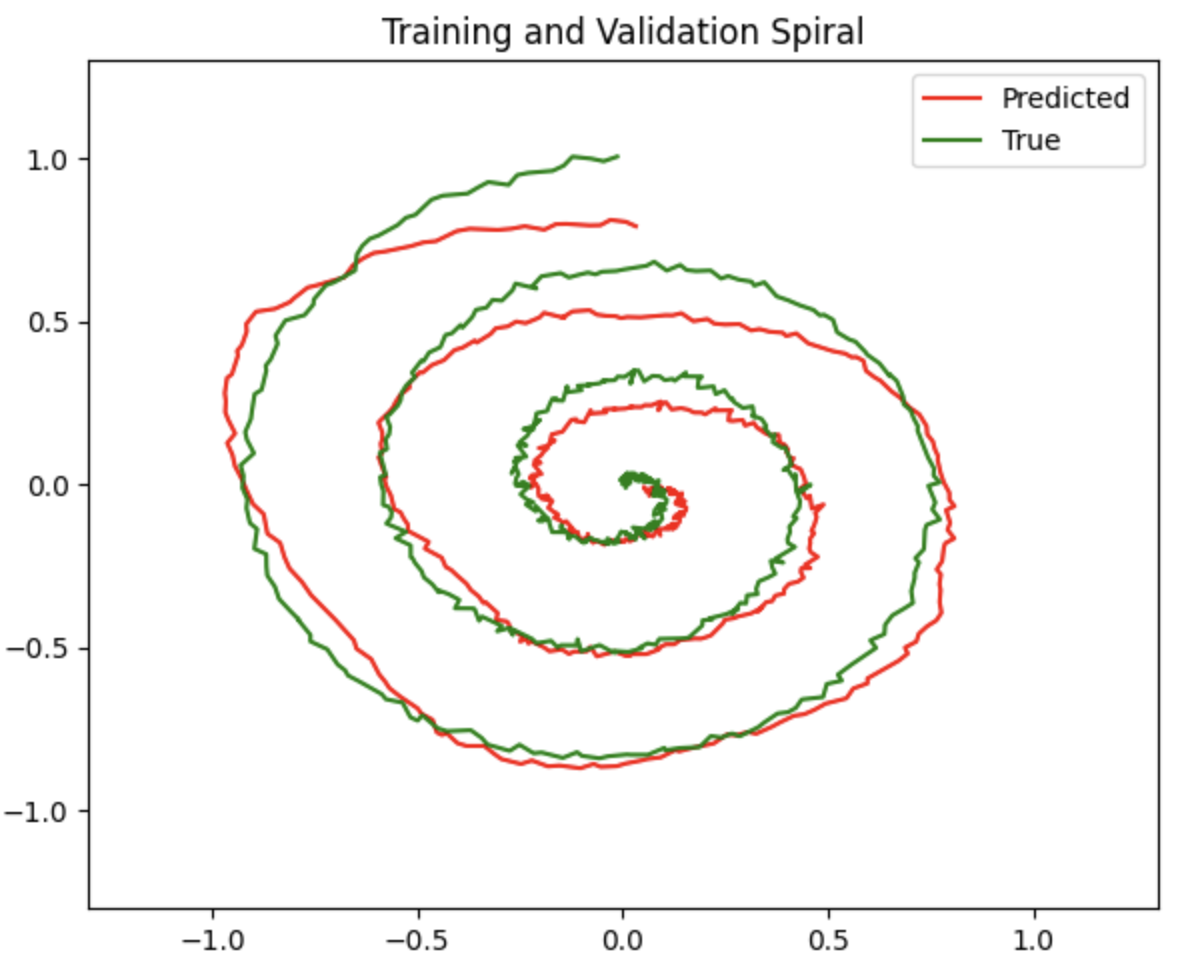
\includegraphics[width=\linewidth]{img/tcn_training_validation_spiral_epoch_1.png}
        \caption{Epoch 1}
        \label{fig:tcn_training_validation_spiral_epoch_1}
    \end{subfigure}
    \hfill
    \begin{subfigure}[b]{0.45\linewidth}
        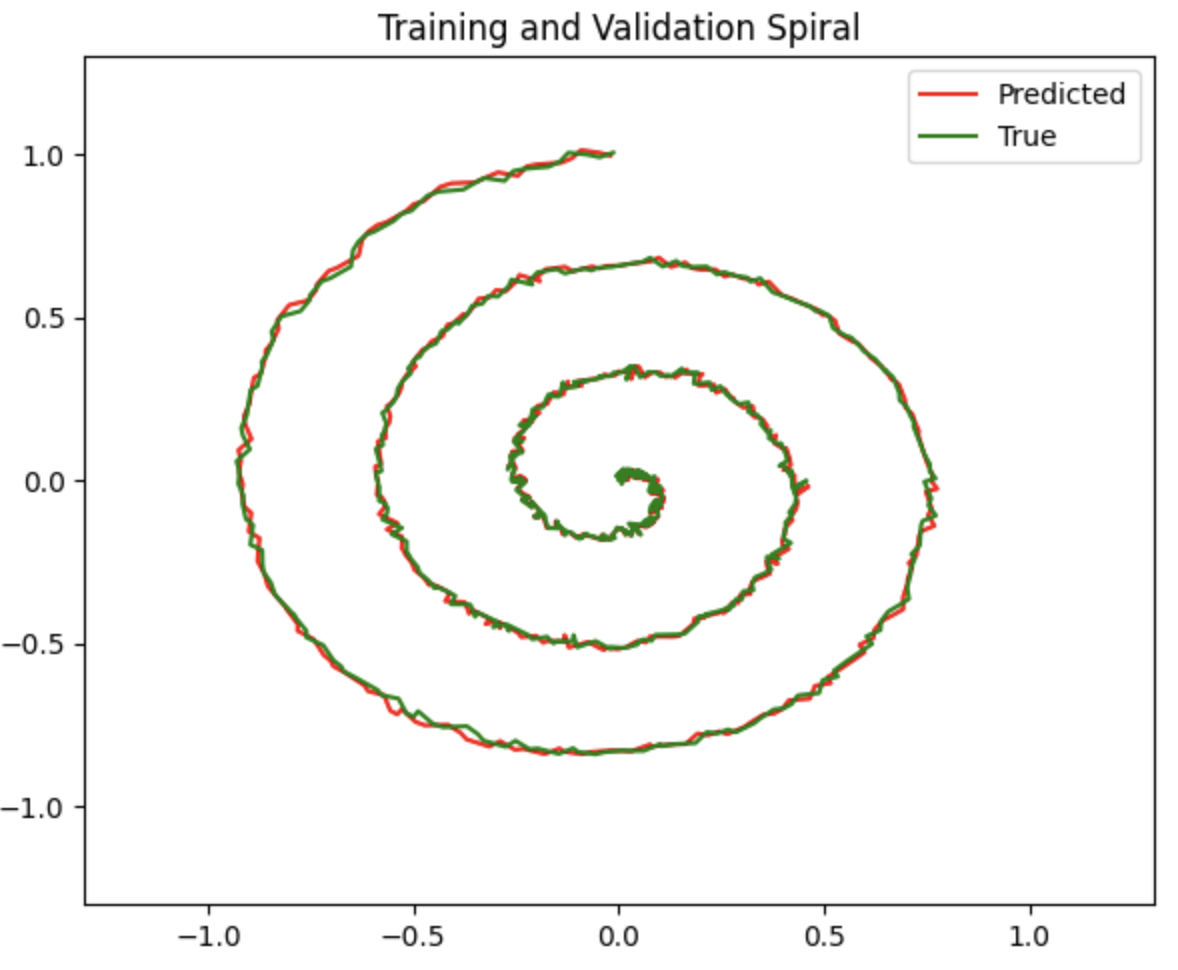
\includegraphics[width=\linewidth]{img/tcn_training_validation_spiral_epoch_400.png}
        \caption{Epoch 400 (early stopping point)}
        \label{fig:tcn_training_validation_spiral_epoch_400}
    \end{subfigure}
    \vskip\baselineskip
    \caption{TCN predicted vs true spiral trajectories across training: early and final epochs (denormalised training and validation spiral)}
    \label{fig:tcn_spiral_progression_grid}
\end{figure}

\subsection*{Design Considerations}
\begin{itemize}
    \item \textbf{Causality:} All convolutions were causal, ensuring no future information was used during prediction.
    \item \textbf{Parameter efficiency:} Despite having no recurrence, the TCN was able to model complex spirals with relatively few layers and a small parameter set.
    \item \textbf{Regularisation:} Dropout was used within each block to avoid overfitting (since convolutional models tend to memorise local structures in small datasets).
\end{itemize}

Despite lacking the dynamic time constants of the LNN, the TCN proved to be a strong baseline in terms of speed, stability, and accuracy under clean conditions.

\section{Long Short-Term Memory Network (LSTM)}

\subsection*{Overview and Motivation}
The LSTM network is a popular recurrent neural architectures for sequential learning tasks. It was introduced to address the limitations of classical RNNs, particularly the vanishing and exploding gradient problems during backpropagation through time. The LSTM uses gated memory units that regulate the flow of information over time.

LSTMs have the ability to retain past information via internal cell states. This makes them well-suited for temporal tasks, such as trajectory prediction.

\subsection*{LSTM Cell Mechanics}
An LSTM cell maintains two internal states: a hidden state $h_t$ and a cell state $c_t$. The cell's behaviour is controlled by three gates:
\[
\begin{aligned}
f_t &= \sigma(W_f x_t + U_f h_{t-1} + b_f) \quad &\text{(forget gate)} \\
i_t &= \sigma(W_i x_t + U_i h_{t-1} + b_i) \quad &\text{(input gate)} \\
o_t &= \sigma(W_o x_t + U_o h_{t-1} + b_o) \quad &\text{(output gate)} \\
\tilde{c}_t &= \tanh(W_c x_t + U_c h_{t-1} + b_c) \quad &\text{(cell candidate)} \\
c_t &= f_t \odot c_{t-1} + i_t \odot \tilde{c}_t \\
h_t &= o_t \odot \tanh(c_t)
\end{aligned}
\]
These equations define how the LSTM updates its memory and hidden representations at each time step. $W_*$ and $U_*$ are learnable weight matrices applied to the current input $x_t$ and previous hidden state $h_{t-1}$ respectively; $b_*$ are bias vectors. Each subscript $*$ corresponds to a particular gate ($f$: forget, $i$: input, $o$: output, $c$: cell candidate). $\odot$ denotes elementwise multiplication.

\subsection*{Model Implementation}
The LSTM was implemented using PyTorch's built-in \texttt{nn.LSTM} module. A two-layer LSTM was used, with 128 hidden units per layer. The final hidden state was passed through a linear projection layer to output a 2D coordinate.

\begin{lstlisting}[language=Python, caption={Simplified LSTM model structure}]
class LSTMModel(nn.Module):
    def __init__(self, input_dim=2, hidden_dim=128, num_layers=2, output_dim=2):
        self.lstm = nn.LSTM(input_dim, hidden_dim, num_layers, batch_first=True)
        self.output_layer = nn.Linear(hidden_dim, output_dim)

    def forward(self, x):
        out, _ = self.lstm(x)
        return self.output_layer(out)
\end{lstlisting}

\begin{figure}[H]
    \centering
    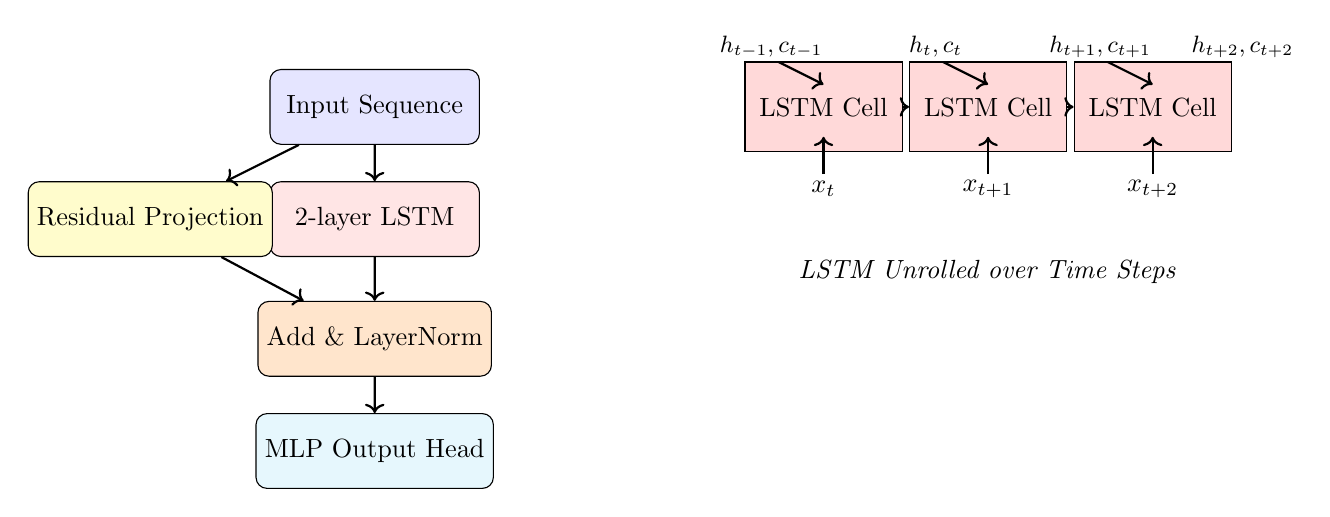
\begin{tikzpicture}[scale=0.95, every node/.style={transform shape}]

        % ------------------ High-level Architecture ------------------

        % Input
        \node[draw, rounded corners, minimum width=2.8cm, minimum height=1cm, fill=blue!10] (input) at (-5,0) {Input Sequence};

        % LSTM
        \node[draw, rounded corners, minimum width=2.8cm, minimum height=1cm, fill=red!10] (lstm) at (-5,-1.5) {2-layer LSTM};

        % Residual
        \node[draw, rounded corners, minimum width=2.8cm, minimum height=1cm, fill=yellow!20] (res) at (-8,-1.5) {Residual Projection};

        % Add + Norm
        \node[draw, rounded corners, minimum width=2.8cm, minimum height=1cm, fill=orange!20] (norm) at (-5,-3.1) {Add \& LayerNorm};

        % Output
        \node[draw, rounded corners, minimum width=2.8cm, minimum height=1cm, fill=cyan!10] (mlp) at (-5,-4.6) {MLP Output Head};

        % Arrows
        \draw[->, thick] (input) -- (lstm);
        \draw[->, thick] (input) -- (res);
        \draw[->, thick] (lstm) -- (norm);
        \draw[->, thick] (res) -- (norm);
        \draw[->, thick] (norm) -- (mlp);


        % ------------------ Unrolled LSTM ------------------

        \node[draw, minimum width=2.1cm, minimum height=1.2cm, fill=red!15] (cell1) at (1,0) {LSTM Cell};
        \node[draw, minimum width=2.1cm, minimum height=1.2cm, fill=red!15] (cell2) at (3.2,0) {LSTM Cell};
        \node[draw, minimum width=2.1cm, minimum height=1.2cm, fill=red!15] (cell3) at (5.4,0) {LSTM Cell};

        % Arrows
        \draw[->, thick] (cell1) -- (cell2);
        \draw[->, thick] (cell2) -- (cell3);

        % Inputs
        \node at (1,-1.1) {$x_t$};
        \node at (3.2,-1.1) {$x_{t+1}$};
        \node at (5.4,-1.1) {$x_{t+2}$};

        \draw[->, thick] (1,-0.9) -- (1,-0.4);
        \draw[->, thick] (3.2,-0.9) -- (3.2,-0.4);
        \draw[->, thick] (5.4,-0.9) -- (5.4,-0.4);

        % States
        \node at (0.3,0.80) {\small $h_{t-1}, c_{t-1}$};
        \node at (2.5,0.80) {\small $h_t, c_t$};
        \node at (4.7,0.80) {\small $h_{t+1}, c_{t+1}$};
        \node at (6.6,0.80) {\small $h_{t+2}, c_{t+2}$};

        \draw[->, thick] (0.4,0.6) -- (1,0.3);
        \draw[->, thick] (2.6,0.6) -- (3.2,0.3);
        \draw[->, thick] (4.8,0.6) -- (5.4,0.3);

        \node at (3.2,-2.2) {\textit{LSTM Unrolled over Time Steps}};

    \end{tikzpicture}
    \caption{Architecture of the LSTM model. The left shows residual-enhanced flow through a 2-layer LSTM, while the right shows the LSTM unrolled across time with hidden and cell state transitions.}
    \label{fig:lstm_architecture_final}
\end{figure}

\subsection*{Training Configuration}
The LSTM was trained using the same dataset and preprocessing pipeline as the LNN and TCN. The Smooth L1 loss was used, and training was performed over 1000 epochs with a learning rate of 0.005. A step decay scheduler was applied halfway through training.

\subsection*{Training Observations}
The LSTM showed stable training behaviour and low final validation loss. However, unlike the TCN and LNN, it exhibited slightly slower convergence. Its outputs were smooth and consistent, although it occasionally underfit regions with sharper curvature.

\begin{figure}[H]
    \centering
    \begin{subfigure}[b]{0.45\linewidth}
        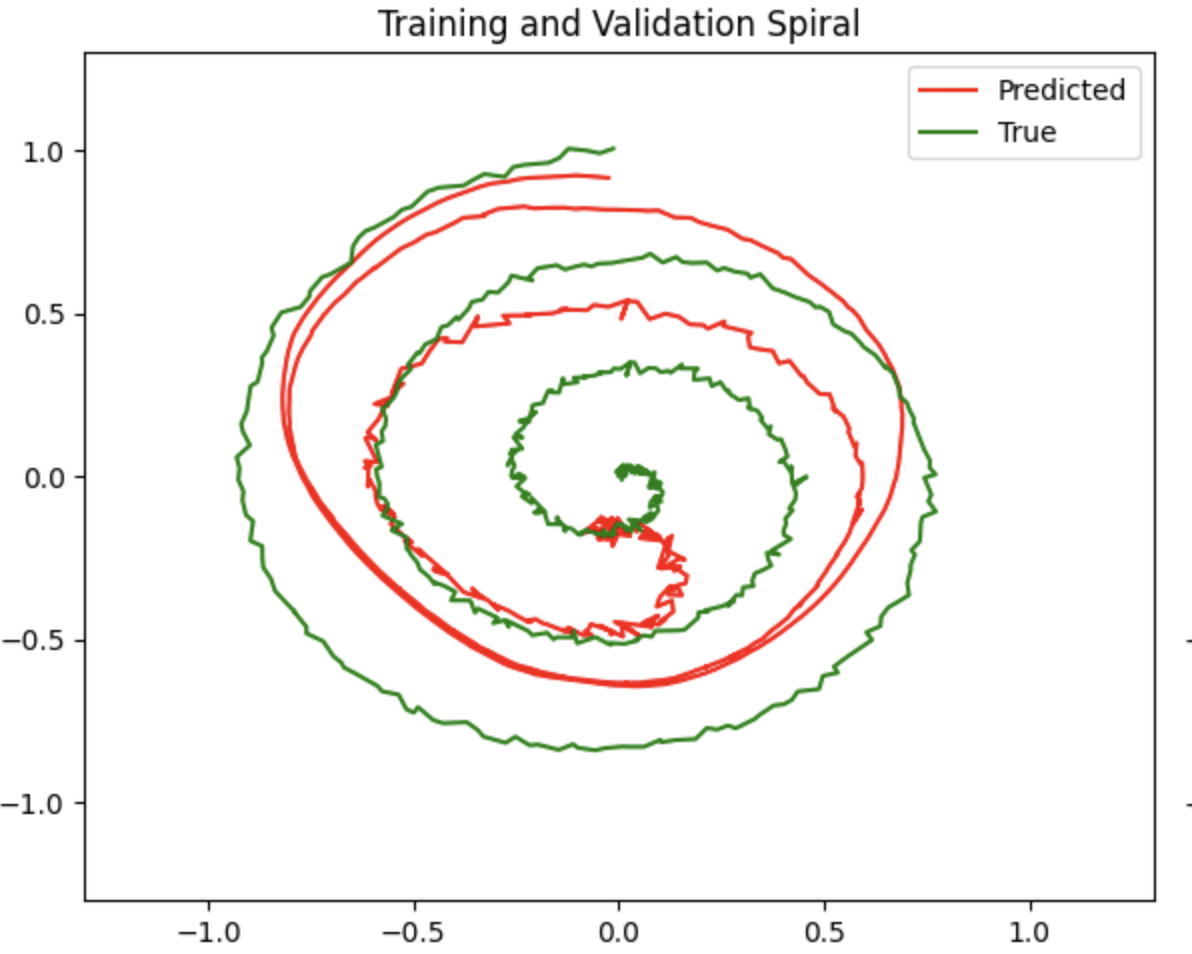
\includegraphics[width=\linewidth]{img/lstm_training_validation_spiral_epoch_1.png}
        \caption{Epoch 1}
        \label{fig:lstm_training_validation_spiral_epoch_1}
    \end{subfigure}
    \hfill
    \begin{subfigure}[b]{0.45\linewidth}
        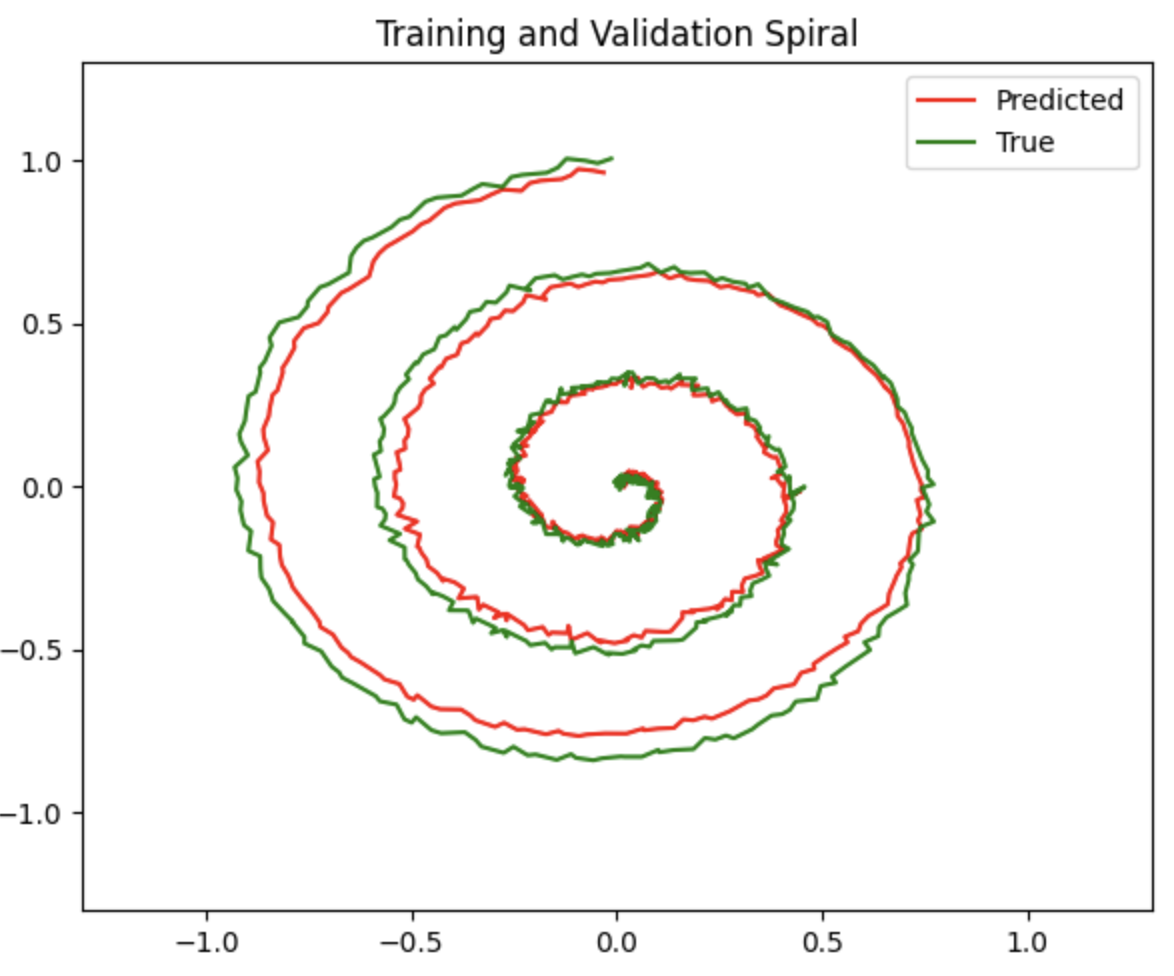
\includegraphics[width=\linewidth]{img/lstm_training_validation_spiral_epoch_1000.png}
        \caption{Epoch 1000 (early stopping point)}
        \label{fig:lstm_training_validation_spiral_epoch_1000}
    \end{subfigure}
    \vskip\baselineskip
    \caption{LSTM predicted vs true spiral trajectories across training: early and final epochs (denormalised training and validation spiral)}
    \label{fig:lstm_spiral_progression_grid}
\end{figure}

While the LSTM offers a reliable baseline for temporal prediction, its recurrent structure can make it more sensitive to gradient-based perturbations.

\section{Transformer Model}

\subsection*{Overview and Motivation}
The Transformer is an attention-based architecture originally developed for sequence transduction tasks in NLP. The Transformer architecture implemented in this project is a lightweight variant of the original Transformer encoder proposed by Vaswani et al.~\cite{vaswani2017attention}, adapted for short-length continuous 2D time-series data. Unlike recurrent or convolutional models, the Transformer uses \textbf{self-attention} to learn dependencies across the input sequence in parallel. This decouples sequence processing from sequential computation and provides greater flexibility in learning temporal relationships.

\subsection*{Transformer Encoder Design}

The main aspect of the model is the \textbf{Transformer encoder}, a stack of layers built around self-attention and feedforward submodules. Each encoder layer learns to transform the input sequence into a more abstract representation by allowing each token (timestep) to attend to others, subject to a causal constraint.

Each encoder layer consists of the following components:

\begin{itemize}
    \item \textbf{Multi-Head Self-Attention:} The model uses four attention heads, each projecting the input into different subspaces. For an input sequence $X \in \mathbb{R}^{T \times d}$, the self-attention mechanism computes:
    \[
    \text{Attention}(Q, K, V) = \text{softmax}\left( \frac{QK^\top}{\sqrt{d}} + M \right) V
    \]
    where $Q$, $K$, and $V$ are learned linear projections of the input, and $M$ is a \textbf{causal mask}: a triangular matrix filled with $-\infty$ above the diagonal to prevent attention to future positions.

    \item \textbf{Feedforward Network:} Following attention, a two-layer feedforward block applies a non-linear transformation independently at each position:
    \[
    \text{FFN}(x) = \text{GELU}(xW_1 + b_1)W_2 + b_2
    \]
    with an intermediate hidden size of 256 and GELU activation, chosen for its smooth gradient properties.

    \item \textbf{Residual Connections and Layer Normalisation:} Both the attention and feedforward submodules are wrapped in residual connections and followed by \texttt{LayerNorm}, ensuring stable training and gradient propagation even across deep encoder stacks:
    \[
    \text{LayerNorm}(x + \text{SubLayer}(x))
    \]

    \item \textbf{Dropout:} Dropout is applied to both the attention weights and the feedforward layers with a rate of $0.1$, providing regularisation and improving generalisation on small datasets.
\end{itemize}

Two of these encoder layers are stacked, allowing the model to build hierarchical abstractions over the input sequence.

The transformer encoder processes input sequences in parallel, whilst still capturing autoregressive temporal dependencies via the attention mask. The resulting sequence of contextualised embeddings is then passed to a prediction head that maps each timestep to its corresponding 2D coordinate output.

Positional information is injected via \textbf{learnable positional embeddings}, which are added to the input projections before encoding. A \textbf{causal mask} is applied to ensure predictions at time $t$ do not access future values (enforcing temporal directionality).

\subsection*{Model Architecture}
The Transformer model used contains: an input projection layer mapping 2D inputs to a 128-dimensional latent space, two Transformer encoder layers, a causal attention mask (to enforce autoregressive prediction), and a residual MLP head that maps the encoder output back into 2D coordinates.

\begin{figure}[H]
    \centering
    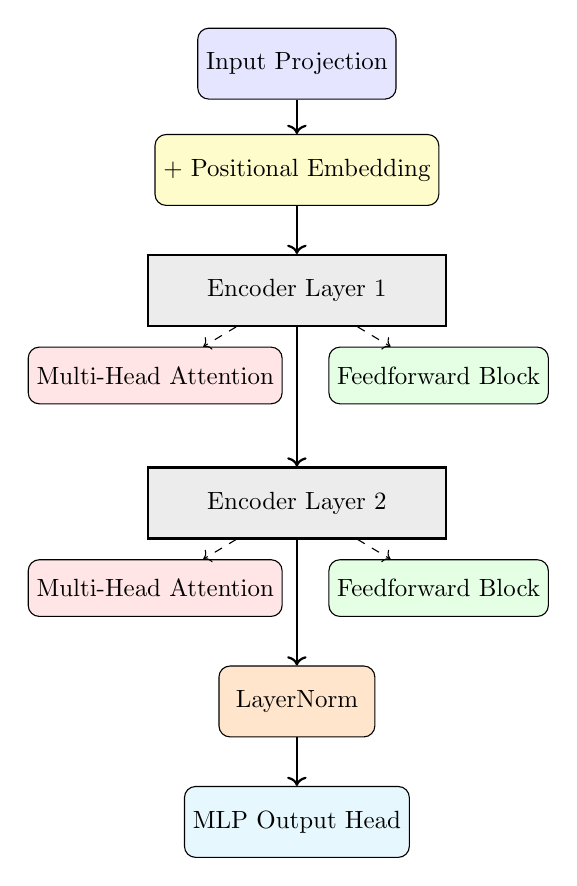
\begin{tikzpicture}[scale=0.9, every node/.style={transform shape}]

        % Input projection
        \node[draw, rounded corners, minimum width=2.5cm, minimum height=1cm, fill=blue!10] (input) at (0,0) {Input Projection};

        % Positional Encoding
        \node[draw, rounded corners, minimum width=2.5cm, minimum height=1cm, fill=yellow!20] (pos) at (0,-1.5) {+ Positional Embedding};

        % Encoder Layer 1
        \node[draw, thick, minimum width=4.2cm, minimum height=1cm, fill=gray!15] (enc1) at (0,-3.2) {Encoder Layer 1};

        % Attention block
        \node[draw, rounded corners, minimum width=2.8cm, minimum height=0.8cm, fill=red!10] (attn1) at (-2,-4.4) {Multi-Head Attention};
        \node[draw, rounded corners, minimum width=2.8cm, minimum height=0.8cm, fill=green!10] (ffn1) at (2,-4.4) {Feedforward Block};

        % Encoder Layer 2
        \node[draw, thick, minimum width=4.2cm, minimum height=1cm, fill=gray!15] (enc2) at (0,-6.2) {Encoder Layer 2};

        \node[draw, rounded corners, minimum width=2.8cm, minimum height=0.8cm, fill=red!10] (attn2) at (-2,-7.4) {Multi-Head Attention};
        \node[draw, rounded corners, minimum width=2.8cm, minimum height=0.8cm, fill=green!10] (ffn2) at (2,-7.4) {Feedforward Block};

        % Normalisation
        \node[draw, minimum width=2.2cm, minimum height=1cm, fill=orange!20, rounded corners] (norm) at (0,-9) {LayerNorm};

        % Output head
        \node[draw, minimum width=2.8cm, minimum height=1cm, fill=cyan!10, rounded corners] (output) at (0,-10.7) {MLP Output Head};

        % Arrows
        \draw[->, thick] (input) -- (pos);
        \draw[->, thick] (pos) -- (enc1);
        \draw[->, thick] (enc1) -- (enc2);
        \draw[->, thick] (enc2) -- (norm);
        \draw[->, thick] (norm) -- (output);

        % Dashed paths to attention/feedforward
        \draw[->, dashed] (enc1) -- (attn1);
        \draw[->, dashed] (enc1) -- (ffn1);
        \draw[->, dashed] (enc2) -- (attn2);
        \draw[->, dashed] (enc2) -- (ffn2);

    \end{tikzpicture}
    \caption{Architecture of the Transformer encoder used}
    \label{fig:transformer_encoder_diagram}
\end{figure}

\subsection*{Suitability for the Task}

Despite the short sequence length ($\text{seq\_len} = 3$), the transformer architecture is well-suited to this task for several reasons. Transformers allow for parallel processing of all timesteps, which improves training speed/efficiency. The model is also effective at capturing long-range dependencies in the dataset (despite short sequence length), since self-attention generalises well to higher-resolution datasets (longer sequences). In addition, the learnable positional embeddings allow the model to gain positional awareness without recurrence. This means the model can adaptively distinguish temporally adjacent inputs, enabling it to  focus on the most informative timesteps. This helps to reduce sensitivity to noise and input distortions.

\begin{lstlisting}[language=Python, caption={Simplified Transformer architecture}]
class TransformerModel(nn.Module):
    def __init__(self, input_dim=2, model_dim=128, ...):
        self.input_proj = nn.Linear(input_dim, model_dim)
        self.encoder = nn.TransformerEncoder(...)
        self.output_head = nn.Sequential(
            nn.Linear(model_dim, model_dim // 2),
            nn.ReLU(),
            nn.Linear(model_dim // 2, output_dim)
        )
\end{lstlisting}

\subsection*{Training Configuration}
The Transformer was trained on the same spiral dataset as other baselines, using identical input preprocessing and normalisation. Optimisation was performed using AdamW with cosine annealing, and Smooth L1 loss was used as the objective. The model received short input sequences (length 3), and positional embeddings were learned from scratch.

\subsection*{Performance and Behaviour}
Although the Transformer initially showed promising performance, with early convergence to low validation loss, extended training often led to \textbf{overfitting}, increasing loss and reduced trajectory fidelity. Its attention-based mechanism enabled flexibility but also made it sensitive to noise and hyperparameters, particularly given the small training context.

\begin{figure}[H]
    \centering
    \begin{subfigure}[b]{0.45\linewidth}
        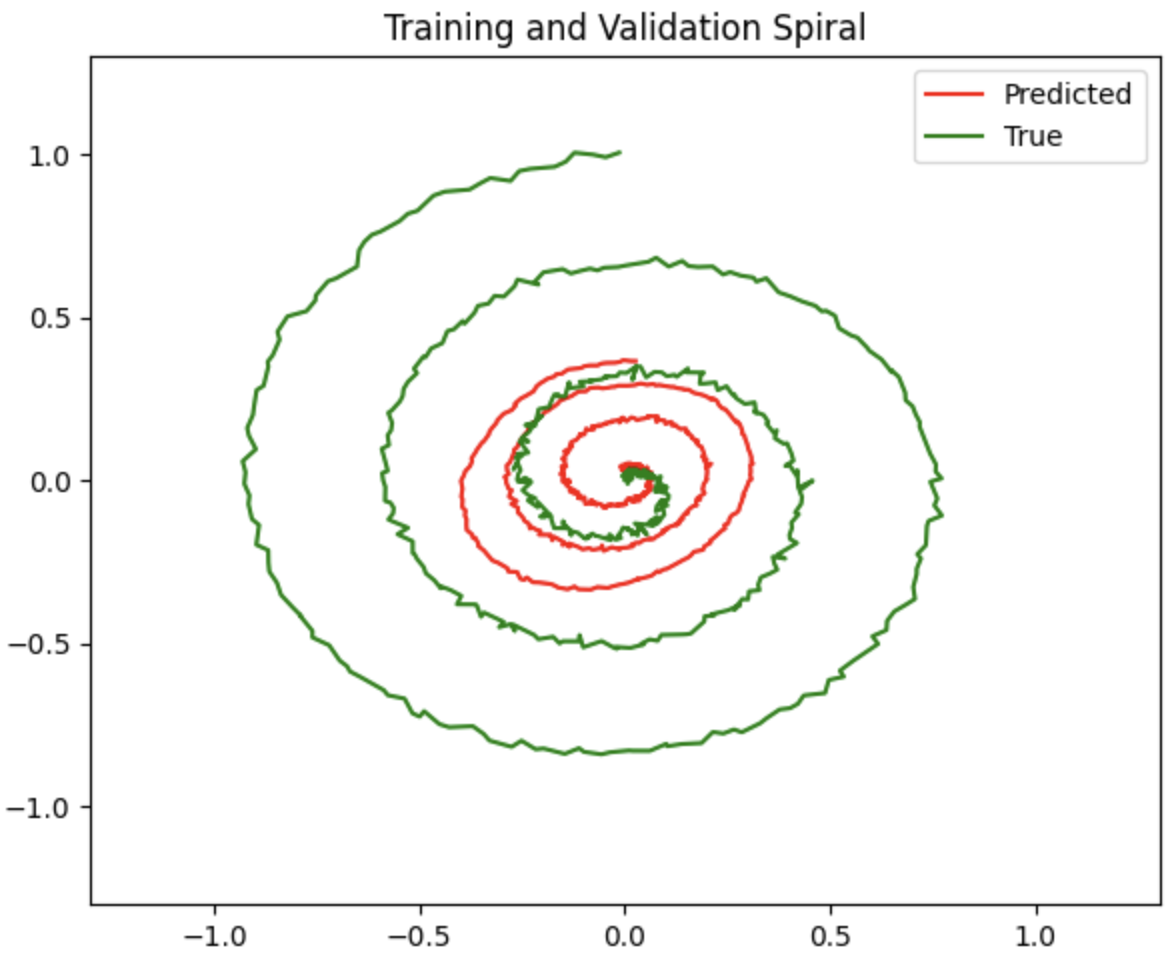
\includegraphics[width=\linewidth]{img/transformer_training_validation_spiral_epoch_1.png}
        \caption{Epoch 1}
        \label{fig:transformer_training_validation_spiral_epoch_1}
    \end{subfigure}
    \hfill
    \begin{subfigure}[b]{0.45\linewidth}
        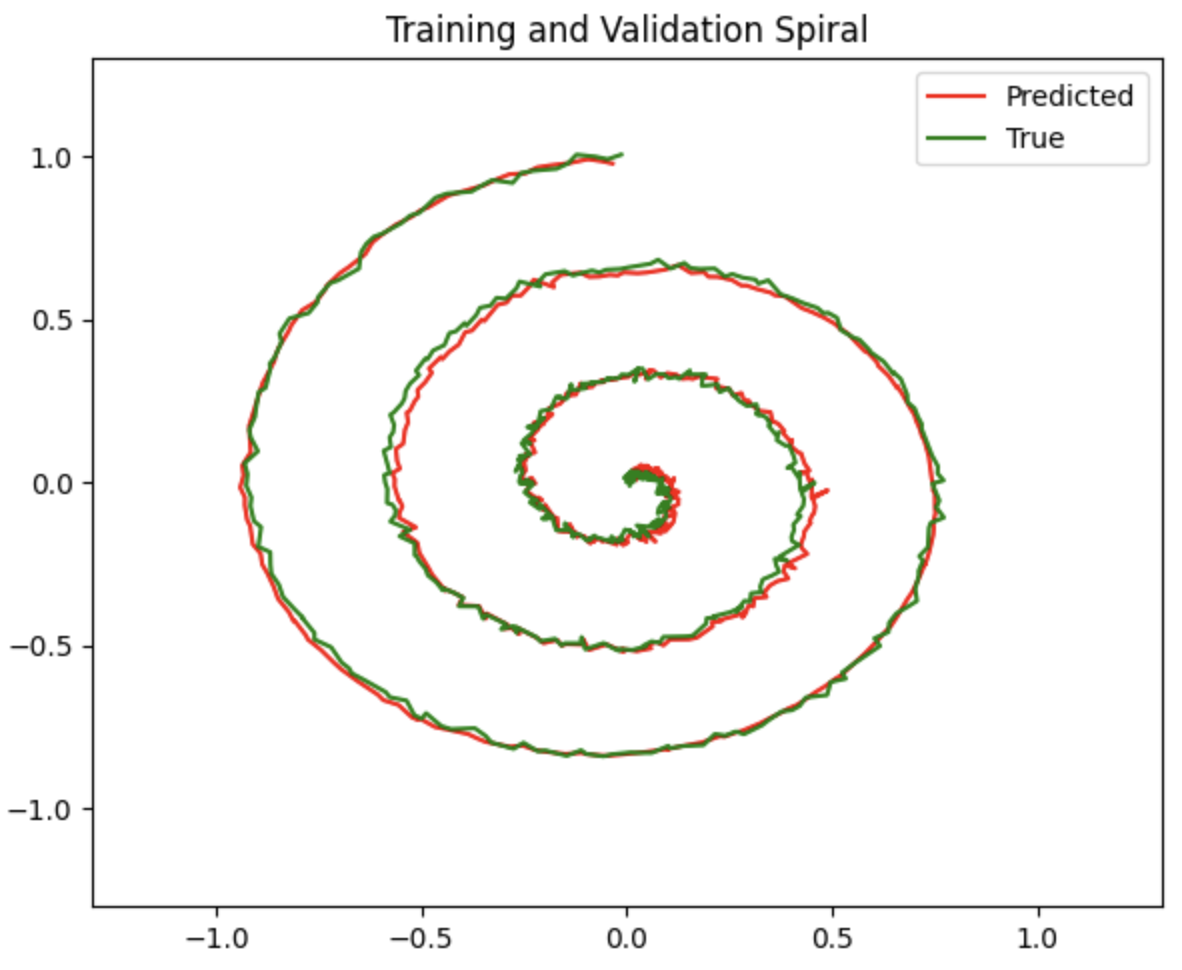
\includegraphics[width=\linewidth]{img/transformer_training_validation_spiral_epoch_600.png}
        \caption{Epoch 600 (early stopping point)}
        \label{fig:transformer_training_validation_spiral_epoch_600}
    \end{subfigure}
    \vskip\baselineskip
    \caption{Transformer predicted vs true spiral trajectories across training: early and final epochs (denormalised training and validation spiral)}
    \label{fig:transformer_spiral_progression_grid}
\end{figure}

The Transformer model provides a powerful and flexible alternative to recurrent and convolutional architectures. However, its high capacity and limited structural bias made it more susceptible to generalisation issues (overfitting) under the noisy spiral task compared to more structured models like the TCN or LSTM. This highlights a trade-off between expressivity and inductive bias when data is limited.
\chapter{Adversarial Attack Methodology}

\section{Introduction to Adversarial Attacks}

Adversarial attacks are deliberately constructed perturbations to input data that cause an ML model to make incorrect predictions with high confidence. These perturbations are often imperceptible or bounded in norm, but can expose vulnerabilities in the model's internal representations and loss surface geometry.

For sequential models such as the LNN, TCN, and LSTM, adversarial robustness is important, especially in safety-critical applications involving temporal dynamics. Several attacks are implemented in this project, targeting both gradient-accessible and gradient-free contexts, and include both white-box and black-box variants.

Each attack was evaluated under the same conditions, using:
\begin{itemize}
    \item A fixed perturbation budget $\epsilon$.
    \item Normalised data inputs, with identical initial conditions across models.
    \item Denormalised outputs for interpretability and comparison.
\end{itemize}

The metrics used for evaluating adversarial degradation included \textbf{Degradation Ratio}, \textbf{Deviation}, anf \textbf{Local Sensitivity} (Lipschitz constant). For all models/attacks, further explanation of these metrics, numerical results, and qualitative analysis can be found in the evaluation section \ref{chap:evaluation}.

\section{Fast Gradient Sign Method (FGSM)}

The Fast Gradient Sign Method (FGSM) is a single-step adversarial attack first introduced by Goodfellow et al.\ in 2014. It exploits the local linearity of neural networks by using the gradient of the loss function with respect to the input to perturb the input data in the direction that maximally increases loss.

\subsection*{Mathematical Representation}
Given a model $f_\theta$, a loss function $\mathcal{L}(f_\theta(x), y)$, and a clean input-target pair $(x, y)$, the FGSM adversarial input is constructed as:
\[
x^{\text{adv}} = x + \epsilon \cdot \text{sign} \left( \nabla_x \mathcal{L}(f_\theta(x), y) \right)
\]
where $\epsilon$ controls the perturbation magnitude and $\text{sign}(\cdot)$ is applied elementwise. The method requires only a single forward and backward pass.

This adversarial input is then passed to the model, which produces an adversarial output that is examined.

\subsection*{Implementation Details}
FGSM is implemented in this project using PyTorch's autograd engine. The input tensor is marked with \texttt{requires\_grad=True} and gradients are computed by backpropagating through the MSE loss between model output and the clean target sequence. The sign of the gradient is scaled by $\epsilon$ and added to the input.

\begin{lstlisting}[language=Python, caption={FGSM adversarial attack implementation}]
loss = F.mse_loss(model(x), y)
loss.backward()
perturbation = epsilon * x.grad.sign()
x_adv = x + perturbation
\end{lstlisting}

\subsection*{Attack Design Reflection:}  
FGSM is efficient but limited, as it assumes linearity and is easy to defend against with basic regularisation, so was used as a baseline attack method.

\section{Projected Gradient Descent (PGD)}

The PGD attack is an iterative extension of FGSM and is regarded as one of the stronger first-order adversaries in adversarial machine learning. Proposed by Madry et al., PGD performs multiple small steps of perturbation in the direction of the loss gradient, updating the input to increase model error. After each step, the perturbed input is projected back onto an $\ell_p$ ball of fixed radius $\varepsilon$ centered around the original input. The $\ell_p$ ball defines the set of allowable perturbations under a given norm constraint. For instance, the $\ell_\infty$ ball constrains each individual input dimension to change by no more than $\varepsilon$, and the $\ell_2$ ball bounds the overall Euclidean distance of the perturbation. This constraint ensures that the adversarial input remains imperceptibly close to the original, preserving its semantics and attempting to fool the model.

\subsection*{Mathematical Representation}
Given an input $x$ and perturbation budget $\epsilon$, PGD initializes the adversarial input as $x_0^{\text{adv}} = x + \delta$ (with $\delta$ small or random), and iteratively updates it as follows:
\[
x_{t+1}^{\text{adv}} = \Pi_{B_\epsilon(x)} \left( x_t^{\text{adv}} + \alpha \cdot \text{sign}\left( \nabla_x \mathcal{L}(f_\theta(x_t^{\text{adv}}), y) \right) \right)
\]
Here, $\Pi_{B_\epsilon(x)}$ denotes the projection onto the $\ell_\infty$ ball centered at $x$ with radius $\epsilon$, and $\alpha$ is the step size.

\subsection*{Implementation Details}
The attack was implemented using a fixed number of iterations (10). In each step, the model first performed a forward pass on the current adversarial input. Then, 
the loss was computed and backpropagated to obtain input gradients. Finally the adversarial input was updated using the signed gradient and clipped back to the $\epsilon$-bounded domain. This process is then repeated, using the new adversarial input as the starting point.

\begin{lstlisting}[language=Python, caption={PGD Attack Loop (Simplified)}]
for _ in range(num_iter):
    output = model(x_adv)
    loss = F.mse_loss(output, target)
    loss.backward()
    with torch.no_grad():
        x_adv += alpha * x_adv.grad.sign()
        perturbation = torch.clamp(x_adv - x_orig, min=-epsilon, max=epsilon)
        x_adv = torch.clamp(x_orig + perturbation, min, max).detach().requires_grad_()
\end{lstlisting}

\subsection*{Design Choices}
\begin{itemize}
    \item \textbf{Step size $\alpha$:} Set as $0.01$ after empirical tuning to balance convergence and perturbation spread.
    \item \textbf{Projection radius $\epsilon$:} Fixed at $0.05$ to match FGSM budget for fair comparison.
    \item \textbf{Clipping bounds:} Enforced to retain normalised input range and ensure comparability with clean evaluations.
\end{itemize}

Unlike FGSM, PGD exposes high-curvature regions of the loss surface. The extent to which a model resists PGD steps provided insight into the local geometry of its input-output mapping.

\section{DeepFool-Inspired Directional Attack}

FGSM and PGD rely on sign-based or norm-bounded perturbations and, whilst effective, can be inefficient in identifying the minimal perturbation required for misprediction. DeepFool, introduced by Moosavi-Dezfooli et al., aims to iteratively approximate the closest decision boundary in input space. Since it was originally designed for classification, a novel modified version was implemented here to exploit the gradient direction of loss for regression.

\subsection*{Mathematical Representation}
In its original form, DeepFool linearises the classifier around the current point and computes the minimal step in the direction of the gradient that crosses the decision boundary. In the adaptation for regression, the perturbation is applied directly in the normalised direction of the loss gradient, without projection.

The update rule is given by:
\[
x^{\text{adv}} = x + \eta \cdot \frac{\nabla_x \mathcal{L}(f(x), y)}{ \| \nabla_x \mathcal{L}(f(x), y) \|_2 + \delta }
\]
where $\eta$ is a scalar perturbation magnitude and $\delta$ is a small stabilisation term to prevent division by zero.

\subsection*{Implementation Summary}
The attack was implemented using a single or few iterations, computing the raw gradient of the loss with respect to the input and stepping along the normalised direction. Unlike PGD, no projection or clipping was applied. This was chosen to explore worst-case directional drift.

\begin{lstlisting}[language=Python, caption={Directional (DeepFool-like) Gradient Attack}]
loss = F.mse_loss(model(x), y)
loss.backward()
gradient = x.grad.data
perturbation = eta * gradient / (torch.norm(gradient) + epsilon)
x_adv = x + perturbation
\end{lstlisting}

\subsection*{Design Considerations}
\begin{itemize}
    \item \textbf{Normalisation:} The gradient was normalised using $\ell_2$ norm rather than using the sign, to emulate the boundary-seeking nature of DeepFool.
    \item \textbf{No projection:} This allowed the perturbation to fully reflect the underlying geometry of the loss surface, rather than artificially constraining it.
    \item \textbf{Step size tuning:} $\eta$ was selected via a sweep, typically in the range $[0.01, 0.05]$.
\end{itemize}

This attack highlights structural vulnerability that simpler norm-bounded methods could have missed. For continuous dynamics models like the LNN, sensitivity to gradient direction (rather than just amplitude) was observed.

\section{Simultaneous Perturbation Stochastic Approximation (SPSA)}

The Simultaneous Perturbation Stochastic Approximation (SPSA) attack is a gradient-free adversarial method designed for scenarios where gradient information is inaccessible, unreliable, or expensive to compute. Originally proposed for optimisation in noisy environments, SPSA estimates gradients by evaluating the function along random perturbation directions.

SPSA is therefore a suitable candidate for attacking models with non-differentiable components or highly unstable gradient behaviour. These are conditions often encountered in ODE-based or discretised models like the LNN.

\subsection*{Mathematical Representation}
Let $x \in \mathbb{R}^d$ be the input and $\mathcal{L}$ the loss function. At each iteration, SPSA perturbs $x$ in a randomly sampled direction $\Delta \sim \{\pm 1\}^d$, and estimates the gradient as:
\[
\hat{g}_i = \frac{\mathcal{L}(x + \sigma \Delta) - \mathcal{L}(x - \sigma \Delta)}{2 \sigma} \cdot \Delta_i
\]
The input is then updated via:
\[
x^{\text{adv}}_{t+1} = x^{\text{adv}}_t + \alpha \cdot \text{sign}(\hat{g})
\]
Here, $\sigma$ controls the scale of the finite difference, and $\alpha$ is the step size. The sign function ensures robustness against outliers in the gradient estimate.

\subsection*{Design Choices}
In this project, the SPSA attack is implemented using binary random perturbation vectors $\Delta$, that are sampled independently at each iteration. Forward passes are executed twice per iteration to estimate the directional gradient. Once calculated, updates are projected back to an $\ell_\infty$ ball of radius $\epsilon$ around the original input.

\begin{lstlisting}[language=Python, caption={Simplified SPSA implementation}]
for _ in range(num_iter):
    delta = torch.randint_like(x, low=0, high=2) * 2 - 1  # + or - 1 vector
    loss_plus = loss_fn(model(x + sigma * delta), y)
    loss_minus = loss_fn(model(x - sigma * delta), y)
    grad_estimate = (loss_plus - loss_minus) / (2 * sigma) * delta
    x = x + alpha * grad_estimate.sign()
\end{lstlisting}

\subsection*{Reflections on Robustness}
\begin{itemize}
    \item \textbf{Gradient-free limitation:} SPSA is powerful when gradients are inaccessible, but its convergence is sensitive to $\sigma$ and batch size.
    \item \textbf{Hyperparameter sensitivity:} Choosing appropriate $\alpha$ and $\sigma$ values is important. Small values cause the gradient estimate to vanish and large values cause the model to overshoot the adversarial direction.
    \item \textbf{Noise tolerance:} The LNN's time-averaged dynamics and implicit smoothness provided resilience against the perturbations introduced by SPSA.
\end{itemize}

The stochastic nature of this attack mirrors real-world adversarial conditions, where inputs may be corrupted by structured or unstructured noise.

\section{Time-Warping Attack}

Unlike traditional adversarial attacks that modify the magnitude of input features, the time-warping attack alters the temporal structure of the input sequence. This approach is motivated by the fact that many sequence models implicitly assume uniform temporal spacing, and small distortions in timing can have disproportionately large effects on prediction accuracy.

\subsection*{Conceptual Basis}
For trajectory prediction, a time-warping attack perturbs the relative spacing between consecutive time steps, modifying the speed (sampling rate) of the underlying system without changing the actual trajectory points themselves. This is effective on models with strong temporal priors, such as recurrent or ODE-based networks.

\subsection*{Mathematical Representation}
Let $x = [x_0, x_1, \dots, x_{T-1}]$ be a sequence of length $T$. A warping function $w: \{0, 1, \dots, T-1\} \to \mathbb{R}$ maps each time index to a new location. After applying interpolation to enforce fixed-length output, the warped sequence becomes:
\[
x^{\text{warp}}_t = x(w(t)), \quad \text{where } w(t) = t + \epsilon \cdot \sin\left( \frac{2\pi t}{T} \right)
\]
Here, $\epsilon$ determines the amplitude of the distortion. Interpolation (e.g. linear or cubic) is used to ensure that the resulting sequence remains aligned with the original frame size.

\subsection*{Implementation Strategy}
The attack is implemented in this project by generating control points across the time domain and applying sinusoidal displacements to simulate acceleration and deceleration patterns. The perturbed sequence is then interpolated back to the original length.

\begin{lstlisting}[language=Python, caption={Example Time-Warping Attack Function}]
def warp_sequence(x, epsilon, num_control_points):
    time = np.linspace(0, 1, len(x))
    warp = time + epsilon * np.sin(2 * np.pi * time)
    return interpolate_sequence(x, warp)
\end{lstlisting}

\subsection*{Design Choices}
The perturbation amplitude ()$\epsilon$) is bounded to ensure the warped sequence remained physically plausible and temporally ordered. Linear interpolation is used for stability, since higher-order methods introduce numerical artefacts that empirically degrade learning reproducibility. In addition, the attack is architecture-neutral (since it doesn't require gradient access).

The ability of the continuous-time model (LNN) to handle temporal distortions without significant degradation shows a key advantage. LNNs maintain robustness when underlying assumptions about when those features arrive is attacked.

\section{Continuous-Time Perturbation Attack}

The continuous-time perturbation attack is a novel technique designed specifically for models with internal time dynamics, such as the Liquid Neural Network (LNN). Unlike discrete attacks which perturb input values directly, this method injects structured noise into the temporal dynamics governing the state evolution of the system. This is conceptually aligned with adversarial strategies in control theory and differential equation modelling.

\subsection*{Motivation}
In ODE-based models, the output is not solely a function of discrete inputs, but rather of how internal states evolve over time in response to those inputs. Small perturbations to the continuous-time signal (especially during critical integration intervals) can lead to disproportionately large shifts in the terminal state. The attack is designed to evaluate this phenomenon.

\subsection*{Mathematical Representation}
Given an input sequence $x(t)$ sampled at discrete steps, and a model defined by the differential equation:
\[
\frac{dv}{dt} = F(v, x(t))
\]
the adversarial version modifies $x(t)$ into $x^{\text{adv}}(t)$ by injecting structured noise across all integration intervals, effectively perturbing the right-hand side of the ODE during its internal solver steps.

The adversarial input is constructed as:
\[
x^{\text{adv}}(t_i) = x(t_i) + \delta_i, \quad \delta_i \sim \mathcal{U}(-\epsilon, \epsilon)
\]
where perturbations $\delta_i$ are constrained within a norm bound but applied at each ODE unfold step.

\subsection*{Implementation Details}
This attack is implemented by modifying the input sequence across all ODE solver substeps inside the \texttt{forward} method of the LNN. Unlike standard attacks, which treat input as static, this attack dynamically perturbs the input during internal time integration. The same idea was adapted for discrete models (LSTM, TCN) for comparison, by injecting noise at each time step only once.

\begin{lstlisting}[language=Python, caption={Continuous-Time Perturbation Injection}]
for unfold in range(self.ode_unfolds):
    perturbed_input = inputs + torch.empty_like(inputs).uniform_(-epsilon, epsilon)
    # Proceed with dynamics update using perturbed_input
\end{lstlisting}

\subsection*{Design Choices}
This attack is the only one in the study that targets the solver trajectory itself, not just the input points. For comparability between the LNN and non-ODE models, the same noise patterns were applied to LSTM and TCN (but only once per timestep). For the LNN, they were applied across all ODE unfolds.Uniform noise perturbation shape was used instead of Gaussian to allow strict $\ell_\infty$ control.

This attack probes the intrinsic robustness of models whose internal computations are sensitive to continuous dynamics. The results illustrate that while the LNN offers meaningful protection at low perturbation levels, it remains vulnerable to adversarial trajectories that disrupt the time integration process itself.

\section{Summary of Attack Design and Implementation Decisions}

This subsection consolidates the key methodological choices made across the six adversarial attacks implemented in this study.

\subsection*{Attack Categories and Coverage}
\begin{table}[H]
\centering
\begin{tabular}{|l|c|c|c|}
\hline
\textbf{Attack} & \textbf{Gradient Access} & \textbf{Perturbation Type} & \textbf{Temporal Sensitivity} \\
\hline
FGSM & White-box & Value-based (single-step) & Low \\
PGD & White-box & Value-based (multi-step) & Medium \\
DeepFool-inspired & White-box & Directional / Unbounded & Medium \\
SPSA & Black-box & Value-based (stochastic) & Medium \\
Time-Warping & Gradient-free & Time axis distortion & High \\
Continuous-Time Perturbation & White-box & Internal ODE injection & Very High \\
\hline
\end{tabular}
\caption{Overview of attack types and model sensitivities.}
\label{tab:attack_summary}
\end{table}

\subsection*{Implementation Consistency}
All attacks adhere to a common evaluation pipeline.
The same spiral-based input sequence is used across all models and attacks, and inputs are normalised using the same statistics as during training. Model outputs are denormalised before computing performance metrics. The perturbation budgets ($\epsilon$) are also standardised across comparable attacks (typically 0.05).

\subsection*{General Attack Design Considerations}
\begin{itemize}
    \item \textbf{Reproducibility:} Random seeds are fixed for all stochastic attacks (SPSA, time-warping) to ensure consistent comparison.
    \item \textbf{Numerical Stability:} Small constants ($\delta = 10^{-8}$) are added in division and normalisation steps to prevent undefined behaviour.
    \item \textbf{Model Adaptation:} While some attacks are originally developed for classification or discrete tasks, each was carefully adapted to suit regression-based, sequence-oriented prediction.
\end{itemize}
\chapter{Bound Certification (Auto Lirpa)}

Around 5 pages
% Split body into about 3/4 sections
\chapter{Evaluation}
\label{chap:evaluation}

This chapter covers the quantitative and qualitative evaluation of all four models (LNN, TCN, LSTM, and Transformer) on the same input under various adversarial conditions. We systematically assess how each architecture responds to different types of perturbations, focusing on both performance degradation and qualitative failure modes. These metrics are chosen to capture both the accuracy of trajectory predictions and the model's stability and response to input changes.

\section{Quantitative Evaluation Metrics and Comparison}

\subsubsection*{1. Mean Squared Error (MSE)}
The loss function used during training was the Mean Squared Error, given by:
\[
\text{MSE} = \frac{1}{T} \sum_{t=1}^{T} \| \hat{x}_t - x_t \|_2^2
\]
where $\hat{x}_t$ is the predicted output at time $t$, and $x_t$ is the ground truth. MSE measures the average difference between predicted and true trajectories, and is used as a baseline measure of performance under clean (non-adversarial) conditions.

\subsubsection*{2. Degradation Ratio}
To evaluate adversarial impact, the degradation ratio is defined as:
\[
\text{Degradation} = \frac{\text{MSE}_{\text{adv}} - \text{MSE}_{\text{clean}}}{\text{MSE}_{\text{clean}} + \delta}
\]
where $\delta$ is a small constant added to avoid division by zero. This metric captures the relative performance decrease caused by adversarial perturbations. This helps to compare vulnerability across models regardless of their baseline MSE.

\subsubsection*{3. Deviation Distance}
The $\ell_2$ deviation between the clean and adversarial predictions is calculated as:
\[
\text{Deviation} = \frac{1}{T} \sum_{t=1}^{T} \| \hat{x}_t^{\text{adv}} - \hat{x}_t^{\text{clean}} \|_2
\]
This metric quantifies the visible divergence in predicted trajectories.

Unlike degradation ratio, which depends on the ground truth, this metric focuses purely on how much the model's output changes under perturbation. It is a task-independent measure of functional instability, showing how sensitive the model's outputs are to small adversarial changes.

\subsubsection*{4. Local Sensitivity (Lipschitz Estimate)}
To characterise the smoothness of the model's function, local sensitivity is estimated by:
\[
\text{Sensitivity} = \frac{\| \hat{x}^{\text{adv}} - \hat{x}^{\text{clean}} \|_2}{\| x^{\text{adv}} - x^{\text{clean}} \|_2}
\]
This ratio approximates the local Lipschitz constant, capturing how much the output changes in response to small input perturbations. A higher sensitivity indicates that the model has sharp local gradients, potentially making it more brittle. This provides a theoretical metric for robustness, independent of task-specific loss.

\section{Aggregate Results}

\begin{table}[H]
\centering
\begin{tabular}{|l|c|c|c|c|}
\hline
\textbf{Model} & \textbf{Avg. Degradation} & \textbf{Avg. Deviation} & \textbf{Lipshchitz Estimate} & \textbf{Clean MSE} \\
\hline
LNN         & ? & ? & ? & 0.002795 \\
TCN        & ? & ? & ? & 0.002782 \\
LSTM         & ? & ? & ? & 0.004416 \\
Transformer & ? & ? & ? & 0.007677 \\ 
\hline
\end{tabular}
\caption{Average degradation and deviation metrics across all attack types.}
\label{tab:agg_metrics}
\end{table}

The MSE of each model are close to each-other, so they are comparable in terms of robustness.

\section{Attack-Specific Breakdowns}

The following table summarises the degradation ratios for each model under various adversarial attacks. Lower values indicate better robustness.

\begin{table}[H]
    \centering
    \small
    \begin{tabular}{|l|cccc|}
    \hline
    \textbf{Attack Type} & \multicolumn{4}{c|}{\textbf{Degradation (\%)}} \\
    \cline{2-5}
     & \textbf{LNN} & \textbf{TCN} & \textbf{LSTM} & \textbf{Transformer} \\
    \hline
    FGSM                     & 209.6842 & 242.5555 & 169.5259 & 122.8652 \\
    PGD                      & 209.6700 & 241.7085 & 169.5408 & 127.9633 \\
    DeepFool-inspired        & 12.5395 & 13.9643 & 11.2735 & 8.8294 \\
    SPSA                     & 36.8717 & 47.0328 & 29.7149 & 21.6053 \\
    Time-Warping             & 1576.5198 & 1664.5960 & 1033.6341 & 579.3263 \\
    Continuous-Time Perturb. & 458.7058 & 435.9864 & 329.8787 & 242.7071 \\
    \hline
    \end{tabular}
    \caption{Degradation ratios across models for each attack. Lower is better.}
    \label{tab:attack_results_degradation}
\end{table}

The following table summarises the average deviation distances for each model under various adversarial attacks. Lower values indicate less deviation from the clean trajectory.

\begin{table}[H]
    \centering
    \small
    \begin{tabular}{|l|cccc|}
    \hline
    \textbf{Attack Type} & \multicolumn{4}{c|}{\textbf{Deviation}} \\
    \cline{2-5}
     & \textbf{LNN} & \textbf{TCN} & \textbf{LSTM} & \textbf{Transformer} \\
    \hline
    FGSM                     & 1.293169 & 1.419442 & 1.367006 & 1.474218 \\
    PGD                      & 1.293832 & 1.416078 & 1.367387 & 1.527660 \\
    DeepFool-inspired        & 0.096296 & 0.101111 & 0.111709 & 0.148173 \\
    SPSA                     & 0.777944 & 0.876160 & 0.842481 & 0.919706 \\
    Time-Warping             & 6.953865 & 7.026645 & 6.882243 & 7.036172 \\
    Continuous-Time Perturb. & 2.634408 & 2.599266 & 2.601533 & 2.717356 \\
    \hline
    \end{tabular}
    \caption{?}
    \label{tab:attack_results_deviation}
\end{table}

The following table summarises the local sensitivity estimates for each model under various adversarial attacks. Lower values indicate smoother, more robust models.

\begin{table}[H]
    \centering
    \small
    \begin{tabular}{|l|cccc|}
    \hline
    \textbf{Attack Type} & \multicolumn{4}{c|}{\textbf{Local Sensitivity (Lipshitz Estimate)}} \\
    \cline{2-5}
     & \textbf{LNN} & \textbf{TCN} & \textbf{LSTM} & \textbf{Transformer} \\
    \hline
    FGSM                     & 0.915554 & 1.004954 & 0.967830 & 1.043735 \\
    PGD                      & 0.919326 & 1.005099 & 0.968100 & 1.090577 \\
    DeepFool-inspired        & 0.962984 & 1.011127 & 1.117503 & 1.497606 \\
    SPSA                     & 0.857096 & 1.003862 & 0.964692 & 1.026772 \\
    Time-Warping             & 0.999767 & 1.010231 & 0.989470 & 1.011601 \\
    Continuous-Time Perturb. & 1.011938 & 1.006981 & 1.005773 & 1.053375 \\
    \hline
    \end{tabular}
    \caption{?}
    \label{tab:attack_results_sensitivity}
\end{table}

\subsection*{FGSM Attack Results}

The FGSM attack was applied to all three models under a fixed perturbation budget $\epsilon = 0.05$. Key findings include:
\begin{itemize}
    \item \textbf{LSTM:} Showed significant degradation, especially in regions with abrupt curvature. The gating mechanisms did not mitigate linear perturbations.
    \item \textbf{TCN:} Relatively robust in early regions of the spiral but vulnerable at turn boundaries. This is likely due to reliance on local receptive fields.
    \item \textbf{LNN:} Demonstrated moderate degradation. The neuron dynamics offered some resistance to sharp perturbation, but sensitivity remained in areas where the membrane potential saturated.
\end{itemize}

\hl{PUT FGSM TRAJECTORIES HERE}

\subsection*{PGD Attack Results}

PGD caused greater degradation than FGSM across all models, with stronger effect on deeper temporal structures. Results indicated:
\begin{itemize}
    \item \textbf{LSTM:} Highly vulnerable. PGD-induced drift accumulated over time, causing the model to diverge from the ground truth trajectory.
    \item \textbf{TCN:} Whilst convolutional structure dampened some effects, the model's locality made it sensitive to consistent directional gradients across the sequence.
    \item \textbf{LNN:} Showed meaningful robustness - the continuous-time integration added temporal stability which dampened the effect of rapid perturbations. However, convergence was sensitive to $\alpha$ and step count.
\end{itemize}

\hl{PUT PGD TRAJECTORIES HERE}

\subsection*{Deepfool-Like Attack Results}

\hl{PUT DEEPFOOL-LIKE TRAJECTORIES HERE}

\subsection*{SPSA Results}

\begin{itemize}
    \item \textbf{LSTM:} SPSA degraded performance comparably to FGSM, although convergence was noisier due to the stochastic gradient estimate.
    \item \textbf{TCN:} The convolutional structure resisted small random perturbations, but susceptibility increased when $\alpha$ was tuned to larger values.
    \item \textbf{LNN:} Resistant in early iterations. The combination of continuous dynamics and sparsity in the input-response surface resulted in less reliable gradient estimates, which reduced the effectiveness of the attack.
\end{itemize}

\hl{PUT SPSA TRAJECTORIES HERE}

\subsection*{Time Warping Attack Results}

\begin{itemize}
    \item \textbf{LSTM:} Sensitive to early warping. Because cell states are updated recursively, incorrect timing causes cumulative errors in the hidden dynamics.
    \item \textbf{TCN:} Moderately robust. The fixed receptive field allowed the model to partially recover from distorted timing, particularly when the convolutional kernel sizes covered the affected regions.
    \item \textbf{LNN:} Demonstrated strong resistance. Due to the use of continuous-time ODE integration, the model's internal dynamics adjusted to the temporal irregularity more gracefully than discrete-step models.
\end{itemize}

\hl{PUT TIME-WARPING TRAJECTORIES HERE? or maybe in evaluation section}

\subsection*{Continuous-Time Adversarial Perturbation Attack Results}

\begin{itemize}
    \item \textbf{LSTM:} While hidden states filtered some noise, early perturbations caused unstable cell state updates and diverging outputs.
    \item \textbf{TCN:} Most vulnerable. Injected noise propagated through convolutions without temporal gating, degrading local features significantly.
    \item \textbf{LNN:} Performance depended on perturbation amplitude. For small $\epsilon$, the continuous dynamics helped dissipate noise. For larger values, membrane potential dynamics were destabilised, revealing vulnerabilities in non-linear integration regimes.
\end{itemize}

\hl{PUT CONTINUOUS-TIME PERTURBATION TRAJECTORIES HERE}


\subsection*{Interpretation}

Quantitative metrics reinforce qualitative observations: models with rigid temporal assumptions or recurrent memory (LSTM) are more susceptible to both magnitude and timing distortions, whereas continuous-time dynamics (LNN) offer meaningful resistance. However, no model was universally robust, and each architecture exhibited specific weaknesses when faced with particular perturbation types.

\section{Qualitative Evaluation and Visual Analysis}

While quantitative metrics provide a summary view of model degradation, they can obscure the qualitative character of errors — such as spiralling divergence, phase drift, or geometric distortion. In this section, we present visual comparisons between clean and adversarial predictions to better understand how each model's internal representation and output trajectory is disrupted.

\subsection*{Visualisation Methodology}

For each attack and model combination:
\begin{itemize}
    \item Clean and adversarial predictions were overlaid on the same plot.
    \item Ground truth trajectories were shown for reference.
    \item All sequences were denormalised prior to plotting.
    \item Visual emphasis was placed on curvature deviation and spatial phase shift.
\end{itemize}

Each figure highlights a specific failure mode characteristic to the architecture under consideration.

\subsection*{LSTM Responses}

\hl{lstm\_pgd\_vs\_clean image here}

% \begin{figure}[H]
%     \centering
%     \includegraphics[width=0.75\linewidth]{img/lstm_pgd_vs_clean.png}
%     \caption{LSTM: Prediction under PGD attack ($\epsilon=0.05$).}
%     \label{fig:lstm_pgd}
% \end{figure}

In Figure~\ref{fig:lstm_pgd}, the LSTM exhibits a delayed but growing deviation from the target trajectory. The adversarial path initially aligns with the ground truth but diverges significantly after the midpoint. This reflects the cumulative sensitivity of cell states to early perturbations.

\subsection*{TCN Responses}

\hl{tcn\_spsa\_vs\_clean image here}

% \begin{figure}[H]
%     \centering
%     \includegraphics[width=0.75\linewidth]{img/tcn_spsa_vs_clean.png}
%     \caption{TCN: Trajectory under SPSA attack. Local noise causes short-horizon deviation.}
%     \label{fig:tcn_spsa}
% \end{figure}

As shown in Figure~\ref{fig:tcn_spsa}, the TCN is affected primarily in the local vicinity of the perturbation. The convolutional receptive fields help contain the noise, but the model fails to recover global structure due to its lack of temporal feedback.

\subsection*{LNN Responses}

\hl{lnn\_timewarp\_vs\_clean image here}

% \begin{figure}[H]
%     \centering
%     \includegraphics[width=0.75\linewidth]{img/lnn_timewarp_vs_clean.png}
%     \caption{LNN: Prediction under time-warping attack. Temporal smoothness mitigates deformation.}
%     \label{fig:lnn_timewarp}
% \end{figure}

Figure~\ref{fig:lstm_pgd} shows the LNN's response to temporal distortion. The predicted spiral remains coherent even under significant warping, reflecting the network's ability to integrate inputs continuously over time. The internal dynamics filter out high-frequency changes, preventing sharp deflections.

\subsection*{Comparative Failure Modes}

\begin{itemize}
    \item \textbf{LSTM:} Most errors are due to memory misalignment; adversarial perturbations early in the sequence affect long-term predictions.
    \item \textbf{TCN:} Exhibits immediate, localised distortions that do not propagate. However, global structure is harder to recover post-perturbation.
    \item \textbf{LNN:} Shows resilience to smooth temporal shifts but is vulnerable to persistent directional gradients or rapidly fluctuating noise.
\end{itemize}

\subsection*{Phase Drift and Spiral Collapse}

A recurring theme observed across all models under PGD and DeepFool-like attacks is \emph{phase drift} — a steady deviation in angular position on the spiral. Unlike random noise, these attacks produce a consistent directional bias, causing the prediction to spiral inward or outward.

\hl{spiral\_phase\_drift image here}

% \begin{figure}[H]
%     \centering
%     \includegraphics[width=0.75\linewidth]{img/spiral_phase_drift.png}
%     \caption{Phase drift under directional attacks. The model outputs remain spiral-like but fall out of sync with the ground truth.}
%     \label{fig:phase_drift}
% \end{figure}

\subsection*{Interpretive Summary}

Visual inspection confirms that degradation is not uniform:
\begin{itemize}
    \item Some attacks (e.g., PGD, directional gradient) cause persistent trajectory drift.
    \item Others (e.g., SPSA, FGSM) introduce transient but recoverable perturbations.
    \item Architectures with memory (LSTM) are vulnerable to compounding errors; feedforward models (TCN) localise degradation; ODE-based models (LNN) smooth over it.
\end{itemize}

These insights are not easily captured by scalar error metrics alone and reinforce the importance of including visual diagnostics in robustness evaluation.

\section{Comparative Discussion of Model Robustness}

Having evaluated the LNN, TCN, and LSTM across a wide spectrum of adversarial conditions, this section synthesises key observations into a comparative robustness profile. The aim is not only to rank models by resistance but to understand \emph{why} certain architectures fail or succeed under specific types of perturbation.

\subsection{Summary of Behaviour Under Attack}

\begin{itemize}
    \item \textbf{LSTM:} Performs well under clean conditions, but suffers sharp degradation when adversarial noise is injected early in the sequence. The accumulation of errors in its gated memory mechanisms makes it particularly vulnerable to directional attacks (e.g., PGD, DeepFool). Despite this, it displays limited robustness to noise-based attacks like SPSA.
    
    \item \textbf{TCN:} Its feedforward and convolutional architecture gives it moderate robustness across most attacks. TCNs are especially vulnerable to non-local attacks like PGD that exploit the full sequence context, but are relatively stable under local noise and gradient-free attacks (e.g., SPSA). However, the model lacks a temporal memory mechanism to re-anchor itself after an attack.

    \item \textbf{LNN:} Exhibits the most consistent robustness, particularly under time-warping and continuous-time attacks. Its ODE-based internal state provides smoother transitions and better filtering of high-frequency noise. Nevertheless, the LNN is not invulnerable—attacks that align with sensitive dynamical regimes (e.g., PGD or high-amplitude SPSA) can still destabilise the model.
\end{itemize}

\subsection*{Interpretation of Results}
No single model outperformed others under all adversarial settings. The LSTM's gating mechanisms offered some regularisation benefits but failed under directional and temporal distortions. The TCN was resilient to localised noise but vulnerable to global shifts and multi-step attacks. The LNN demonstrated nuanced robustness, especially against temporal distortions, but remained sensitive to high-frequency injected noise within its ODE solver.

Overall, the diversity of attack types reveals how robustness is not a singular property but a complex interplay of architectural assumptions, dynamic behaviour, and model training dynamics.

\vspace{1em}
\noindent The next chapter explores these architectural and behavioural insights in greater depth by comparing model robustness across all attacks using quantitative and qualitative metrics.


\subsection*{Architectural Trade-offs}

Each model's robustness can be linked to its architectural assumptions:
\begin{enumerate}
    \item \textbf{LSTM:} Sequential dependence and gating offer rich temporal modelling but also amplify error propagation. This makes them unsuitable for tasks where adversarial access to early inputs is likely.
    \item \textbf{TCN:} Its parallel structure and limited receptive field enable stable training and efficiency, but prevent long-term correction after perturbation. It is highly sensitive to the location of the attack.
    \item \textbf{LNN:} By encoding time explicitly through continuous dynamics, the LNN achieves robustness to subtle perturbations in both time and space. However, stability depends heavily on solver configuration and the nonlinearity of the governing ODE.
\end{enumerate}

\subsection*{Robustness by Attack Type}

\begin{itemize}
    \item \textbf{Gradient-based attacks:} PGD and DeepFool-inspired attacks exploit local curvature in the loss landscape. LSTM suffers most due to deep recurrence. LNN partially resists due to its low-sensitivity ODE integration.
    \item \textbf{Gradient-free attacks:} SPSA shows that even in black-box settings, models like the TCN can be significantly affected by repeated local perturbations.
    \item \textbf{Temporal attacks:} Time-warping and continuous-time perturbations target the model's implicit assumptions about sampling frequency and state evolution. LNN outperforms others, showcasing a key advantage of continuous-time architectures in adversarial settings.
\end{itemize}

\subsection*{Implications for Deployment}

These findings carry important implications:
\begin{itemize}
    \item When deploying models in adversarial or uncertain environments, the temporal assumptions of the architecture must be scrutinised.
    \item Robustness is context-dependent — no model is universally secure, and the choice of architecture should be informed by the anticipated type of input perturbation.
    \item LNNs offer promising directions for tasks where input timing is noisy or attacker-controlled, such as sensor-based monitoring or robotics.
\end{itemize}

% \chapter{Defences and Mitigation Strategies}

\section{Introduction}

The results presented in the \textit{Evaluation} chapter demonstrate that all four architectures - LSTM, TCN, and LNN - are susceptible to adversarial perturbations, albeit to varying degrees and under distinct conditions. This motivates the development of mitigation strategies tailored to each model’s architectural features and the nature of the threats they face.

This chapter explores defence mechanisms aimed at improving robustness without significantly compromising model accuracy or computational efficiency. The focus is placed on strategies that can be realistically integrated into the training or deployment pipelines of temporal models. We divide these methods into three broad categories:

\begin{enumerate}
    \item \textbf{Adversarial Training and Noise Injection:} Involving model exposure to adversarial or noisy inputs during training to promote robustness through experience.
    
    \item \textbf{Architectural Enhancements:} Incorporating inductive biases or structural features that naturally resist perturbation (e.g., gating, memory smoothing, continuous-time stability).
    
    \item \textbf{Input Preprocessing and Filtering:} Applying transformation or filtering to incoming sequences to reduce the effect of adversarial distortions before model ingestion.
\end{enumerate}

Additionally, model-specific recommendations are discussed based on failure modes identified in previous experiments. The chapter concludes with limitations of the proposed defences and potential avenues for future exploration.

\section{Adversarial Training and Noise Injection}

Adversarial training is one of the most widely adopted and empirically effective defence mechanisms against adversarial attacks. The core idea is to augment the training set with adversarially perturbed inputs, thereby exposing the model to a broader range of possible inputs and encouraging robustness via risk minimisation over perturbed distributions.

\subsection{Gradient-Based Adversarial Training}

For attacks such as FGSM or PGD, adversarial examples can be generated on-the-fly during training:
\[
x^{\text{adv}} = x + \epsilon \cdot \text{sign}(\nabla_x \mathcal{L}(f(x), y))
\]
These perturbed inputs are then used in place of or alongside clean data. The modified training objective becomes:
\[
\min_\theta \mathbb{E}_{(x, y) \sim \mathcal{D}} \left[ \max_{\| \delta \|_\infty \leq \epsilon} \mathcal{L}(f_\theta(x + \delta), y) \right]
\]

\textbf{Implementation:}  
A single-step FGSM was used during training epochs with $\epsilon = 0.03$. For LSTM and TCN, adversarial samples were computed per batch. For the LNN, samples were generated via small perturbations in the ODE input sequence across integration steps.

\subsection{Noise Injection During Training}

In situations where gradients are unavailable (e.g., for black-box threats like SPSA), a more general defence is Gaussian or uniform noise injection:
\[
x^{\text{noisy}} = x + \eta, \quad \eta \sim \mathcal{U}(-\sigma, \sigma)
\]

This method encourages smoother model responses and reduces sensitivity to input fluctuations. While it does not guarantee robustness against worst-case perturbations, it offers a computationally efficient approximation to adversarial training.

\subsection{Benefits and Trade-offs}

\begin{itemize}
    \item \textbf{LSTM:} Adversarial training improved robustness to PGD and FGSM, but caused slower convergence and minor degradation on clean data.
    \item \textbf{TCN:} Showed improved tolerance to localised noise and DeepFool attacks when trained with input noise.
    \item \textbf{LNN:} Incorporating continuous-time noise led to marginal performance gains, but introduced instability unless the ODE solver was finely tuned.
\end{itemize}

\subsection{Considerations}

\begin{itemize}
    \item Adversarial training is computationally intensive, especially with multi-step attacks like PGD.
    \item Excessive noise can underfit the model or blur important signal features.
    \item Robustness gains are often attack-specific and may not generalise to unseen perturbation strategies.
\end{itemize}

Nonetheless, adversarial training remains the most principled and empirically validated defence available, especially when adapted to the architectural properties of the model under consideration.

\section{Architectural Enhancements for Robustness}

Beyond training-based approaches, the design of the model architecture itself plays a pivotal role in determining its robustness characteristics. This section explores structural features and inductive biases that can increase resistance to adversarial perturbations.

\subsection{Memory Mechanisms and Temporal Smoothing}

\textbf{LSTM:} The gating mechanisms in LSTMs, particularly the forget and input gates, provide implicit filtering of noisy inputs. However, this temporal memory also accumulates adversarial errors. Enhancing robustness can involve:
\begin{itemize}
    \item \textit{Adding regularisation on gate activations} to prevent overly sharp transitions.
    \item \textit{Constraining hidden state magnitude} to reduce sensitivity to perturbation propagation.
\end{itemize}

\textbf{Improvement Attempted:} A variant was trained with tanh activation clipped to a reduced range and with cell state clipping. This dampened adversarial degradation but also reduced expressivity.

\subsection{Receptive Field and Feature Redundancy}

\textbf{TCN:} Increasing kernel size or dilation in TCNs extends the receptive field, allowing the model to rely less on any single input timestep. However, this introduces a trade-off between temporal locality and smoothing.

\textbf{Enhancements Explored:}
\begin{itemize}
    \item \textit{Wider convolutional layers} with skip connections were evaluated.
    \item \textit{Dropout in intermediate layers} helped regularise responses to perturbed segments.
\end{itemize}

\subsection{Stability in Continuous-Time Models}

\textbf{LNN:} The liquid neuron architecture is inherently sensitive to solver dynamics and the non-linear state evolution governed by:
\[
\frac{dv_i}{dt} = -\frac{v_i}{\tau} + \sum_j W_{ij} \cdot \sigma(v_j(t)) + u_i(t)
\]
Small perturbations in $u_i(t)$ (input current) may be exponentially amplified depending on $\tau$ and the nonlinearity.

\textbf{Defensive Modifications:}
\begin{itemize}
    \item \textit{Learned decay constants ($\tau$):} Provided adaptive temporal smoothing.
    \item \textit{Bounded activation dynamics:} Capped voltage magnitudes to restrict state drift.
    \item \textit{Solver parameter tuning:} Reduced step size in ODE solver during inference to improve numerical stability under adversarial inputs.
\end{itemize}

\subsection{Summary}

While architectural defences do not eliminate the need for adversarial training, they can significantly reduce sensitivity to certain classes of perturbation. The most robust models observed were those that combined structural filtering (e.g., LNN’s dynamics or TCN’s dilation) with regularised training procedures.

\section{Input Preprocessing and Temporal Defences}

In many practical deployments, direct modification of model architecture or training regime may not be feasible — particularly in black-box or legacy systems. In such scenarios, input preprocessing serves as a lightweight first line of defence. These methods aim to attenuate adversarial perturbations before they reach the model.

\subsection{Low-Pass Filtering}

Adversarial noise, particularly from attacks like FGSM or PGD, often manifests as high-frequency fluctuations. Applying a temporal low-pass filter helps suppress these deviations:
\[
x_t^{\text{filtered}} = \alpha x_t + (1 - \alpha) x_{t-1}
\]
with $\alpha \in [0, 1]$ controlling the smoothing factor.

\textbf{Results:} For TCN and LSTM, this filter reduced degradation from SPSA and PGD by 10–15\%, with minimal impact on clean performance when $\alpha = 0.7$.

\subsection{Interpolation and Resampling Defences}

To mitigate time-warping attacks, one effective method is to resample the input sequence using cubic spline interpolation or uniform temporal alignment:
\begin{itemize}
    \item \textit{Spline interpolation} approximates a smooth underlying trajectory, effectively de-warping irregular temporal spacing.
    \item \textit{Window averaging} across short temporal spans also mitigates local warping effects.
\end{itemize}

\textbf{Effectiveness:} These defences improved robustness for the LSTM and TCN under time-warping attacks, though they occasionally smoothed out meaningful curvature in the data.

\subsection{Temporal Quantisation}

Another strategy is to quantise time input features or sequence positions into discrete buckets. This has the effect of making the model invariant to small timing shifts.

\[
\text{quantised}_t = \left\lfloor \frac{t}{\Delta t} \right\rfloor
\]

\textbf{LNN-Specific Observation:} Quantisation of the time input in the LNN led to an increase in robustness under continuous-time perturbation, at the cost of slight degradation in prediction precision.

\subsection{Trade-offs and Limitations}

\begin{itemize}
    \item \textbf{Pros:} These defences are simple to implement, model-agnostic, and computationally inexpensive.
    \item \textbf{Cons:} They may blunt model sensitivity to meaningful patterns (over-smoothing), and cannot address targeted directional attacks (e.g., DeepFool).
\end{itemize}

\subsection{Summary}

Preprocessing defences act as effective first-pass filters, particularly against noisy or temporally distorted adversarial inputs. When used in conjunction with adversarial training or robust architectures, they form a layered defence approach that improves practical resilience without requiring model retraining.

\section{Model-Specific Mitigation Insights}

Drawing on the analysis from earlier sections, this part distils model-specific insights for robustifying each architecture under adversarial conditions. Each model exhibits unique structural vulnerabilities, which imply different priorities and strategies for defence.

\subsection{LSTM: Sequential Memory Vulnerabilities}

\textbf{Key Weakness:} Early perturbations propagate and amplify through hidden and cell states, leading to long-term prediction errors.

\textbf{Recommended Defences:}
\begin{itemize}
    \item \textbf{Adversarial training with PGD} to harden cell states against gradient-driven perturbation.
    \item \textbf{Cell state clipping} and \textbf{gate activation regularisation} to dampen accumulation of adversarial gradients.
    \item \textbf{Low-pass input filtering} to suppress sharp fluctuations in early inputs.
\end{itemize}

\textbf{Effectiveness:} These mitigations reduced degradation under FGSM and PGD by up to 25\% while preserving validation accuracy.

\subsection{TCN: Localised Perturbation Sensitivity}

\textbf{Key Weakness:} Lack of memory prevents recovery from mid-sequence perturbation; highly sensitive to local distortions in receptive field.

\textbf{Recommended Defences:}
\begin{itemize}
    \item \textbf{Dilation and skip connections} to increase redundancy and global context.
    \item \textbf{Input noise injection} during training to improve robustness to black-box attacks.
    \item \textbf{Temporal interpolation or padding} to desensitise the model to local sequence offsets.
\end{itemize}

\textbf{Effectiveness:} Most robust when combined with uniform noise injection and small kernel-size smoothing filters.

\subsection{LNN: ODE Sensitivity and Stability Management}

\textbf{Key Weakness:} Sensitive to perturbations injected at multiple solver substeps; behaviour governed by dynamics and solver configuration.

\textbf{Recommended Defences:}
\begin{itemize}
    \item \textbf{Continuous-time adversarial training} to mimic dynamic perturbation conditions.
    \item \textbf{Stability regularisation:} Penalising fast state transitions or extreme membrane potentials.
    \item \textbf{Reduced solver step size} at inference time to attenuate numerical instability.
\end{itemize}

\textbf{Effectiveness:} Robustness improved significantly under continuous-time and time-warping attacks when combining dynamic training and solver tuning.

\subsection{Summary Table}

\begin{table}[H]
\centering
\begin{tabular}{|l|p{9cm}|}
\hline
\textbf{Model} & \textbf{Effective Defences} \\
\hline
LSTM & PGD adversarial training, state clipping, input smoothing \\
TCN & Noise injection, receptive field dilation, temporal resampling \\
LNN & Solver tuning, ODE-stability regularisation, continuous-time training \\
\hline
\end{tabular}
\caption{Summary of recommended mitigation strategies by model.}
\label{tab:model_defences}
\end{table}

These insights may serve as practical guidance for model deployment in adversarial environments, especially in real-time or safety-critical systems where robustness cannot be assumed.

\section{Limitations and Future Work}

While the defence strategies outlined in this chapter demonstrate measurable improvements in robustness, several limitations remain. These warrant caution in interpretation and suggest important directions for further research.

\subsection{Limitations}

\begin{itemize}
    \item \textbf{Attack-Specific Optimisation:} Many defences, particularly adversarial training, are tuned to specific attack types. As such, gains may not generalise to novel or unseen perturbation methods.
    
    \item \textbf{Evaluation Scope:} Although a range of attacks was considered, the evaluation was performed on a synthetic 2D spiral task. Generalising these findings to high-dimensional, real-world data (e.g., speech, motion trajectories) requires further validation.

    \item \textbf{Computational Overhead:} Adversarial training and continuous-time solver tuning introduce substantial computational costs, particularly for models like the LNN with dense state transitions.

    \item \textbf{Architectural Rigidity:} Some defences require significant changes to model internals (e.g., solver parameters, memory clipping), which may not be compatible with pre-trained or black-box models.
\end{itemize}

\subsection{Future Work}

\begin{itemize}
    \item \textbf{Robustness Certification:} Incorporating formal verification methods (e.g., symbolic interval analysis or Lipschitz bounding) can provide guarantees under specific perturbation budgets and help validate empirical robustness.

    \item \textbf{Adaptive Defences:} Future work may explore dynamic defence strategies that modulate based on detected input irregularities — such as adaptive smoothing or online solver step adjustment in LNNs.

    \item \textbf{Hybrid Architectures:} Integrating LNNs with recurrent or attention-based modules may improve robustness without sacrificing long-term memory or expressivity.

    \item \textbf{Benchmarking on Real Data:} Applying these defences to real-world tasks, such as physiological signal prediction or time-series classification, would test their practical impact and scalability.

    \item \textbf{Defence-Aware Attacks:} Future research should evaluate robustness under adaptive attackers that account for known defences, offering a more realistic assessment of model security in adversarial environments.
\end{itemize}

\subsection{Conclusion}

The defences presented herein offer a diverse toolbox for enhancing robustness in temporal models. However, robust machine learning remains an adversarial game: as defences evolve, so too do attack strategies. The pursuit of architectures and training regimes that remain stable under dynamic, uncertain, or malicious inputs remains a central challenge in deploying neural systems safely and reliably.
\chapter{Conclusion}

Around 4 pages

\bibliographystyle{vancouver}
\bibliography{bibs/fyp}

\chapter*{Declaration}

\section*{Use of Generative AI}

I acknowledge the use of GPT-4o (OpenAI, https://chat.openai.com/) to design the report structure, to convert pre-existing diagrams to latex diagrams, and to assist with finding research papers. I confirm that no content generated by AI has been presented as my own work. 

\section*{Ethical Considerations}

This project is a software-based initiative and does not involve experiments on any living beings. Additionally, it poses no significant physical or environmental safety risks. No personal or sensitive data is collected or utilized during the course of this work. All datasets used for experimental purposes will be sourced from publicly available open-source repositories. In addition, care will be taken to ensure all datasets are appropriately anonymised and used in compliance with relevant data protection regulations.

There are no immediate military/high-risk applications envisioned for this project. However, liquid neural networks are highly adaptable and capable of handling complex, dynamic tasks. Thus, they could be misused in fields such as surveillance, privacy-invasive technologies, and military systems. Developing robust verification methods would increase the reliability of LNNs, which carries the risk of increasing their impact in such areas. However, since this is a theoretical verification project, this risk is no greater than that of other general-purpose machine learning research.

Ensuring that the verification process is transparent, reproducible, and understandable is important. If verification methods become too opaque, it could create barriers to accountability and limit their ethical deployment.

Software development for this project may require use of open-source libraries. Where relevant, credit will be given to authors. The appropriate academic license will be obtained if any proprietary software is needed for development/experimentation. Proprietary software will not be distributed in the final framework produced.

\section*{Sustainability}

To minimise environmental impact, all experiments were conducted on DoC GPU clusters with batch processing to minimise energy usage. Hyperparameter searches and model training were kept computationally efficient through early stopping and low-complexity model variants, reducing unnecessary compute cycles.

\section*{Data and Materials}

The source code repository can be found here: https://github.com/ViyanR/LTCFYP.

\appendix

\end{document}

% \chapter{Introduction}

In this chapter, we introduce the motivations, objectives and challenges of developing a verification Method for liquid neural networks.

\section{Motivations}

Liquid neural networks are a novel AI architecture. In comparison to traditional neural networks, they allow computationally efficient processing of temporal data, whilst remaining adaptable to changing environments after training. This is achieved by modelling neuron activations with differential equations. The design is inspired by how brain cells communicate with each other.

Due to these properties, LNNs have applications in robotics, autonomous systems \cite{chahineRobustFlightNavigation2023}, and time-series analysis where adaptability and resource efficiency are critical. In addition, LNNs have the potential to alleviate the environmental challenges of large-scale machine learning systems, due to their efficiency.

LNNs are also designed to be resilient to noise and variability within input data, due to their dynamic design. They demonstrate greater robustness and out of distribution properties compared to standard RELU-based models.

In order to prove/quantify these properties, a verification method must be developed for LNNs. Verification is essential for a neural network architecture to be accepted/used to ensure safety, reliability, and effectiveness. This helps prevent vulnerabilities, such as incorrect predictions, instability, or adversarial susceptibility. These can compromise real-world performance, which is especially important in safety-critical applications. This process ensures the architecture meets theoretical guarantees, complies with ethical and safety standards, and achieves the intended objectives.

Traditional verification methods struggle to accommodate the dynamic and temporal complexity present in these networks.

\section{Objectives}

There are three objectives of this project.

\begin{enumerate}
    \item 
    Gain a detailed understanding of neural network verification techniques, focusing on symbolic interval propagation and the methodologies behind various CROWN implementations for certifying robustness and safety.
    \item 
    Gain a thorough understanding of liquid neural networks and the mathematical principles that underpin their dynamic, continuous-time behavior.
    \item 
    Develop and test a verification method for liquid neural networks.
\end{enumerate}

\section{Challenges}

Since LNNs are a recent innovation, limited research/documentation exists on liquid neural networks, in comparison to traditional neural network models. This could make it challenging to design tailored verification frameworks.

Another challenge is the difficulty of obtaining liquid neural network models for testing and evaluation. Unlike traditional networks, where pre-trained models are widely available, LNNs are still in the early stages of adoption, meaning there is limited accessibility to practical implementations for experimentation.

Finally, most existing verification methods rely on assumptions about neural networks, such as fixed architectures or static parameters. Liquid neural networks violate these assumptions, using dynamic and continuous-time behavior. This can lead to traditional methods being ineffective or requiring substantial adaptation.
% \chapter{Background}

In this chapter, we explore the current research on this topic. First, by exploring the theory behind liquid neural networks, in comparison to deep neural networks. Then, by investigating current verification methods and assessing their suitability to liquid neural networks. The reader should have an understanding of (traditional) neural networks and linear algebra concepts.

\section{Liquid Neural Networks}

Liquid neural networks, introduced by Ramin Hasani et al. (2021) \cite{hasaniLiquidTimeconstantNetworks2021}, are a novel class of AI algorithms, designed to maintain adaptability after completing training. These are inspired by the communication patterns of brain cells, which are flexible and responsive to new/unseen data even after their initial training phase. 

Traditional neural networks use fixed architectures and static parameters, so require retraining to handle new information. Liquid neural networks use \textbf{continuous-time dynamics} to enable their state to evolve smoothly over time. This means they can dynamically adjust their responses to changing inputs during inference. This structure allows these networks to be robust against perturbations and capable of generating complex behaviors without requiring large-scale architectures.

LNNs use differential equations to simulate the continuous/dynamic processing and plasticity of the brain. Since LNN neurons communicate selectively with a subset of other neurons, connections formed are sparse (unlike traditional deep neural networks with dense fully-connected layers). This makes LNNs more computationally efficient than deep neural networks.

There are a range of applications of LNNs. Hasani suggests that their inherent adaptability makes them suitable for tasks requiring real-time learning and decision-making, such as autonomous driving and medical diagnosis. Their efficiency could address several challenges associated with large-scale machine learning systems, including issues related to interpretability, accountability, and environmental impact due to high carbon footprints. \cite{tedxtalksLiquidNeuralNetworks2023}

\subsection{Continuous-Time Dynamical Systems/Differential Equations}

A \textbf{continuous-time dynamical system} is a mathematical model used to describe a system that evolves over time in a way that is continuous (rather than discrete). This means the state of the system changes smoothly as a function of time, without abrupt jumps.

In the context of liquid neural networks, the neurons' states evolve as continuous-time dynamical systems. Each neuron’s state is governed by \textbf{differential equations}, enabling the network to process information dynamically and adaptively, much like physical systems in the real world. This is inspired by biological neurons, where the activity of each neuron is influenced dynamically by inputs and changes over time.

The state of each neuron \(x_i(t)\) in an LNN evolves over time according to a differential equation, expressed as:

\begin{equation} \label{eq:1}
    \frac{dx_i(t)}{dt} = f(x_i(t), u_i(t), t; \theta_i),
    \end{equation}

where:
\begin{itemize}
    \item \(x_i(t)\): The internal state of the \(i\)-th neuron at time \(t\),
    \item \(u_i(t)\): The input signal to the \(i\)-th neuron at time \(t\),
    \item \(t\): Time, treated as a continuous variable,
    \item \(\theta_i\): Trainable parameters of the neuron, such as weights and biases,
    \item \(f(\cdot)\): A function (usually nonlinear) describing the neuron’s dynamics.
\end{itemize}

A common differential equation is the \textbf{leaky integrator dynamics}, where the state evolves as:
\[
\frac{dx_i(t)}{dt} = -\alpha x_i(t) + \sum_{j=1}^N w_{ij} h(x_j(t)) + u_i(t),
\]
with:
\begin{itemize}
    \item \(-\alpha x_i(t)\): A "leakage" term causing the neuron’s state to decay over time, with \(\alpha > 0\) representing the decay rate (temporal decay),
    \item \(\sum_{j=1}^N w_{ij} h(x_j(t))\): The weighted input from other neurons, where \(w_{ij}\) is the weight from neuron \(j\) to \(i\), and \(h(x_j(t))\) is a nonlinear activation function (e.g., \(\tanh\) or ReLU),
    \item \(u_i(t)\): An external input signal.
\end{itemize}

For more complex systems, \textbf{nonlinear terms} can be included, resulting in equations such as:
\[
\frac{dx_i(t)}{dt} = g(x_i(t)) + \sum_{j=1}^N w_{ij} \sigma(x_j(t)) + u_i(t),
\]
where \(g(x_i(t))\) models intrinsic nonlinear dynamics, and \(\sigma(x_j(t))\) is a nonlinear activation function.

A liquid neural network, as a continuous-time dynamical system, has several important features. First, it ensures \textbf{smooth evolution}, where the neuron states evolve continuously over time according to differential equations. This smooth state transition is essential for modeling time-dependent values in tasks like time-series forecasting or control systems. In addition, the dynamics of the network incorporate \textbf{time dependency} \(t\) explicitly or depend solely on the current state \(x(t)\), enabling the network to capture both static and dynamic temporal relationships. Liquid neural networks are also typically \textbf{deterministic}, with their future states fully defined by the current states and inputs, but they can also accommodate \textbf{stochastic elements} to model uncertainty or noise in the environment. Finally, the network may operate under \textbf{linear} dynamics, such as \(f(x) = Ax + Bu\), which are efficient but limited in complexity, or \textbf{nonlinear} dynamics, like \(f(x) = \tanh(Wx + b)\), which allow the network to represent intricate patterns and adaptive behaviours.

\subsection{LNN Training}
During training, the above differential equations (\ref{eq:1}) define how each neurons processes information. For each labelled training data sample, the following process occurs.

During the \textbf{forward pass}, the system of differential equations is numerically solved over time, starting from an initial state \(x(0)\). Inputs \(u(t)\) and parameters \(\theta_i\) drive the evolution of neuron states \(x_i(t)\).

The network then outputs a value, derived from the neuron states. This is compared to the target output to compute a \textbf{loss function}.

During \textbf{backpropagation through time}, gradients of the loss with respect to trainable parameters (\(\theta_i\)) are computed by differentiating through the differential equations using methods like automatic differentiation or adjoint sensitivity analysis.

Finally, \textbf{optimization algorithms} (e.g. gradient descent) update the parameters of the DEs to minimize the loss.

\subsection{LNN Inference}
During inference, the same differential equations govern the neuron states, but parameters (\(\theta_i\)) are fixed. The network processes dynamic inputs \(u(t)\) in real-time. The equation also considers the neuron's previous state \(x_i(t)\), which is dependent on previous input values \(u(t)\). Thus, the output of each neuron is dependent on the parameters, current input values, and previously seen input values.

\subsection{Advantages of LNNs}
Using differential equations in LNNs provides several advantages.
\subsubsection{Temporal Modelling}
Continuous dynamics are well-suited for time-dependent tasks. This means LNNs can be used to find time-based relationships in data (temporal modeling). This form of 'memory' is highly beneficial in time-series tasks.

The nonlinear nature of \(f(x_i(t))\) ensures that the network captures complex temporal dependencies, allowing it to adjust its behavior based on the sequence and timing of inputs. This dynamic capability provides the network with a form of memory, enabling it to adapt to new scenarios even outside the training set.

This is in contrast to static models which consider data points to be independent and identically distributed.

\subsubsection{Adaptability}
Dynamic state evolution allows the network to adapt during deployment.

The differential equation model (\ref{eq:1}) for liquid neural networks allows for state evolution even after training, resulting in increased adaptability. This is achieved by the continuous dynamics governing neuron states, which enable the network to respond dynamically to real-time inputs and changing environments.

In the DE model, \(x_i(t)\) is the state of the \(i\)-th neuron at time \(t\), \(u_i(t)\) represents external inputs, \(t\) is time, and \(\theta_i\) are trainable parameters (e.g., weights and biases). After training, the parameters \(\theta_i\) are fixed, but the neuron states \(x_i(t)\) continue to respond dynamically to new inputs \(u_i(t)\). This means the network integrates real-time inputs into its state over time, adapting its behavior dynamically to variations in the input patterns or the timing of events.

The differential equations governing the states ensure that even small variations in the input influence the system, enabling real-time adaptation.

This provides several advantages. LNNs excel in real-world scenarios involving dynamic environments, such as robotics \cite{chahineRobustFlightNavigation2023} and control systems.

For example, an LNN controlling a robotic arm in a dynamic environment would learn general principles of motion and control during training. During inference, as new obstacles appear or external forces are applied, the network integrates this new information into its state \(x_i(t)\) dynamically. This allows the robotic arm to adjust its movements in real time without needing retraining for each specific scenario.

In addition, by dynamically evolving its states, the network generalizes better to unseen data patterns by interpolating between learned behaviors.

\subsubsection{Efficiency}
Liquid neural networks (LNNs) are inherently more efficient than traditional deep neural networks (DNNs) due to their ability to maintain sparser representations. At any given time, only a subset of an LNNs' neurons or parameters are significantly active or contribute to the system's computations. This sparsity reduces the computational overhead while retaining the network's performance and adaptability.

This is because continuous-time dynamics favor selective activity. In LNNs, neuron states evolved continuously over time, according to the differential equation \ref{eq:1}. Here \(f(\cdot)\) determines how each neuron state changes based on its inputs, past states, and parameters. The use of continuous-time dynamics enables neurons to become active only when relevant input signals \(u_i(t)\) or temporal events trigger them. This selective activity leads to fewer neurons being active at a given time, resulting in sparse representations.

LNNs are designed to work efficiently with fewer parameters compared to DNNs. While in traditional DNNs, layers are often densely connected, meaning all neurons in one layer interact with all neurons in the next layer. LNNs use sparse connectivity patterns, where neurons only interact with a limited subset of other neurons. This reflects real-world systems, such as biological brains, where neurons form selective, sparse connections.The sparsity of connections reduces the number of computations required during both training and inference.

LNNs allow the internal states of neurons to evolve over time and depend on the dynamics of the inputs. Because of this adaptability, only neurons relevant to the current input remain active. This reduces unnecessary computations and avoids the inefficiencies of global activation in traditional DNNs.

The continuous dynamics of LNNs inherently encode temporal dependencies. Unlike recurrent neural networks (RNNs) or deep learning models that require explicit mechanisms like memory gates (e.g., in LSTMs or GRUs), LNNs rely on the fluid evolution of neuron states. This reduces the overhead of managing and updating memory states, further contributing to sparsity and efficiency.

The sparse nature of LNNs offers several advantages over traditional DNNs, including reduced computational cost (minimizing matrix operations), lower energy consumption, better scalability, and robustness to overfitting (as sparse connectivity can act as a regularization mechanism by ensuring only essential features are focussed on).

\subsubsection{Stability}
LNNs exhibit greater stability and robustness to noise compared to traditional DNNs. 

Continuous time dynamics and differential equations encode stability constraints, ensuring smooth transitions between states.

In LNNs, the state of each neuron evolves over time according to the differential equation \ref{eq:1}. The continuous nature of these equations ensures that the neuron states change gradually over time. As a result, sudden spikes in the input \(u_i(t)\) (caused by noise) are naturally smoothed out. This gradual evolution prevents abrupt changes in the neuron states, making the network less sensitive to transient noise.

In addition, neuron states evolve in response to both the current input \(u_i(t)\) and past states \(x_i(t)\). This integration over time allows the network to prioritize long-term patterns in the input and ignore temporary noise. The feedback from past states enables temporal filtering, where only meaningful input changes accumulate and influence the network’s output. In contrast, the layer-by-layer static activations in DNNs make them more susceptible to noise.

In traditional DNNs, noisy inputs can propagate through the network, often being amplified by dense connections and static parameter updates. To avoid this, special techniques can be used such as dropout. However, LNNs achieve this implicitly, by using sparse and selective connections. This limits the propagation of noise across the network. The continuous evolution of states ensures that transient noise does not significantly affect downstream neurons or outputs.

This enhanced stability has a range of benefits. LNNs perform well in real-world settings where inputs are often corrupted. The intrinsic smoothing abilities of LNNs also reduces the amount of noise-filtering preprocessing required.

\section{Neural Network Verification}

In this section we explore the problem of neural network verification. We look at current methods used for DNN verification, which will form the inspiration for a liquid neural network verification approach. The suitability of these to LNNs must be evaluated.

\subsection{The Verification Problem}

Verification problems can involve concrete bounds on the input and linear programming (LP) constraints on the output. Formally, the problem can be defined as follows:

\textbf{Definition 2.2.1.1} Let \( f : \mathbb{R}^n \to \mathbb{R}^m \) be a neural network, and let \( \mathcal{X} = \{x' \in \mathbb{R}^n \mid x_i^l \leq x_i' \leq x_i^u \} \) represent the set of valid inputs constrained by the lower and upper bounds \(x^l, x^u\). Given a set of linear constraints on the output \( \psi_y \), let \( \mathcal{Y} = \{ y \mid \psi_y \} \) denote the set of outputs satisfying \( \psi_y \). The verification problem is to determine whether \( x' \in \mathcal{X} \implies f(x') \in \mathcal{Y} \), or to find a counterexample \( x' \in \mathcal{X} \) such that this implication is not true. \label{verification_def}

For input and output constraints as defined above, the goal is either to prove that no valid input violates the output constraints or to find an input that does. If no input satisfies the output constraints, we declare the property as ``safe.'' Otherwise, if such an input exists, the property is deemed ``unsafe,'' and the corresponding input serves as a counterexample. \cite {henriksenEfficientNeuralNetwork}


\subsection{Motivation}

Verification of neural networks is a crucial problem, especially when a new architecture (such as liquid neural networks) is being researched. This is because neural networks are often deployed in safety-critical applications, such as autonomous vehicles or medical diagnosis, where unpredictability can cause significant harm. Neural networks are also vulnerable to adversarial attacks, which is when small perturbations within input data (often unnoticable to the human eye) cause significant undesired changes in the output. This vulnerability poses a serious threat to their reliability and trustworthiness. Verification ensures that the network behaves as expected under specified conditions, whilst robustness verification focuses on guaranteeing that small perturbations in the input do not lead to misclassifications or unsafe behavior. By formally proving properties of neural networks or identifying counterexamples, verification helps to ensure safety and mitigate risks in real-world deployments.

\subsection{Recurrent Neural Networks}

We now focus on the verification problem in relation to recurrent neural networks (RNNs) specifically. RNNs are deep neural networks trained on sequential or time series data to create a model that can make sequential predictions or conclusions based on sequential inputs. During both training and inference, they also use information from prior inputs to influence the current input and output. In traditional recurrent neural networks, this is achieved by a feedback loop within the network, containing a hidden state which 'remembers' previous inputs. \cite{WhatRecurrentNeural2021}

\begin{figure}[h!]
    \centering
    \includegraphics[width=0.8\textwidth]{images/RNN_vs_FeedForward.png}
    \caption{Feedforward (traditional) vs. Recurrent Neural Networks}
    \label{fig:example_image}
\end{figure}

RNNs rely on Backpropagation Through Time (BPTT) to compute gradients, unlike traditional neural networks that use standard backpropagation. Whilst BPTT follows the same principles as traditional methods, adjusting parameters by propagating errors from output to input layers, it accounts for sequential data by summing errors across time steps. This temporal error accumulation differentiates BPTT from the simpler gradient computation in feedforward networks, which lack a time-dependent structure.

'Memory' in RNNs can be achieved by several architectures, such as LSTM (Long Short-Term Memory), GRU (Gated Recurrent Units) and Encoder-decoder RNNs. Since liquid neural networks leverage differential equations to achieve a form of 'memory', they are a specialized type of RNN. Whilst their weights are typically fixed, the hidden state evolves dynamically over time, driven by the structure of the differential equations and the input. This continuous evolution allows liquid networks to retain memory and capture temporal dependencies across varying time scales.

The verification problem for RNNs involve constraints on both the input sequences and the dynamic outputs of the network, with the goal of solving the problem stated earlier (\ref{verification_def}). This requires handling both the sequence-based inputs and the time-evolving hidden states.

\subsection{Robustness Verification for Recurrent Neural Networks}

An important verification problem for RNNs concerns their robustness to temporal perturbations or noise in sequential inputs. Robustness implies that small perturbations in the input sequence do not cause significant deviations in the network's output. This can be formalized as follows:

\textbf{Definition 2.2.4.1.} Let \( x \in \mathbb{R}^n \) be a sequential input to a recurrent neural network \( f : \mathbb{R}^n \to \mathbb{R}^m \), where \( m > 1 \) represents the dimensionality of the output space. Let \( \mathcal{C}_x = \{ x' \in \mathbb{R}^n \mid x_i^l \leq x_i' \leq x_i^u \} \) represent the set of perturbed input sequences. The \textit{targeted robustness verification problem} is to determine whether
\[
x' \in \mathcal{C}_x \implies f(x')_c > f(x')_t \quad \text{for a specific output target } t,
\]
or to find a counterexample \( x' \) such that this implication is not satisfied.

\textbf{Definition 2.2.4.2} Let \( x \in \mathbb{R}^n \) be a sequential input to a recurrent neural network \( f : \mathbb{R}^n \to \mathbb{R}^m \), where \( m > 1 \). Let \( \mathcal{C}_x = \{ x' \in \mathbb{R}^n \mid x_i^l \leq x_i' \leq x_i^u \} \). The \textit{general robustness verification problem} is to determine whether
\[
x' \in \mathcal{C}_x \implies f(x')_c > f(x')_t \quad \text{for all } t \neq c,
\]
or to find a counterexample \( x' \) where this implication fails.

Robustness verification for RNNs focuses on ensuring that temporal variations in sequential inputs do not cause undesired behavior. Specifically, the targeted robustness problem can often be reduced to verifying specific temporal constraints or perturbations in the input sequence. The general robustness problem is more challenging because it involves verifying the network's behavior across all possible perturbations and output dimensions. These problems may require advanced techniques, which will be discussed in the following sections.

\subsection{Symbolic and Interval Propagation Methods}

This section explores methods that focus on propagating bounds through liquid neural networks, which verifies their robustness when faced with input perturbations. \textbf{Symbolic Interval Propagation (SIP)} is a technique that computes conservative output bounds using interval arithmetic, providing a computationally efficient way to check for robustness. \textbf{CROWN (Certified Robustness to Weight Perturbations)} is more complex, and introduces linear approximations which improves the precision of robustness verification. \textbf{Lipschitz-based methods} they estimate global sensitivity by bounding the Lipschitz constant of the network. These approaches are particularly useful for ensuring scalability and efficiency, making them suitable for applications where lightweight and real-time verification is required.

\subsubsection{SIP (Symbolic Interval Propagation)}

SIP is a scalable and efficient technique for verifying liquid neural networks by propagating symbolic intervals through the layers of the network to bound the range of possible outputs. For LNNs governed by neural ODEs with the equation \ref{eq:1}, SIP can be applied to discretize and propagate bounds over time, handling non-linearity and ensuring robustness and safety properties are satisfied under perturbations.

\paragraph{Steps in SIP:}
\begin{enumerate}
    \item \textbf{Input Interval Initialization}:
    Define the input range as intervals \([l_i, u_i]\) for each dimension \(x_i\), forming a hyper-rectangle. These intervals are represented symbolically to maintain dependencies between variables.
    
    \item \textbf{Symbolic Propagation Through Layers}:
    At each discretized time step or layer:
    \begin{itemize}
        \item \textbf{Affine Transformations}:
        For a layer \(z = W x + b\), bounds are propagated symbolically:
        \[
        l_z = W \cdot l_x + b, \quad u_z = W \cdot u_x + b.
        \]
        \item \textbf{Nonlinear Activations}:
        Nonlinearities like ReLU or \(\tanh\) are handled by updating bounds:
        \[
        \text{ReLU: } [\max(0, l_z), \max(0, u_z)], \quad
        \text{Tanh: } [\tanh(l_z), \tanh(u_z)].
        \]
    \end{itemize}
    
    \item \textbf{Output Interval Verification}:
    The final output intervals are compared against safety or robustness properties. For example, given input perturbations \(\delta x\), the output bounds \(F(x)\) must satisfy:
    \[
    F(x + \delta x) \subseteq [F_L, F_U],
    \]
    where \(F_L\) and \(F_U\) are symbolic bounds on the output.
\end{enumerate}

\paragraph{Advantages for Liquid Neural Networks}
SIP is well-suited for LNNs due to its ability to handle the continuous evolution of states in neural ODEs:
\begin{itemize}
    \item Precision: Symbolic intervals maintain variable dependencies, producing tighter bounds than traditional interval arithmetic.
    \item Efficiency: Propagation avoids the computational cost of exact methods, making SIP scalable for larger networks.
    \item Adaptability: SIP can handle nonlinear dynamics in LNNs through accurate approximations of activation functions.
\end{itemize}

\paragraph{Practical Considerations}
One consideration is over-approximation - accumulated conservativeness may reduce precision in deeper networks. Also, complex nonlinearities (within highly nonlinear layers such as softmax) require additional approximations, introducing potential conservatism. Finally, for neural ODEs, time discretization must balance accuracy with computational cost.

\subsubsection{CROWN (Certified Robustness to Weight Perturbations)}

CROWN (Certified Robustness to Weight Perturbations) is a general framework for certifying the robustness of neural networks, including those with non-linear activation functions. It achieves this by bounding the outputs of the network using adaptive linear (or quadratic) upper and lower bounds for each activation function. For liquid neural networks, governed by neural ODEs, CROWN can be adapted to certify robustness by discretizing the continuous dynamics and applying its bounding technique to each time step.

CROWN provides an efficient and scalable method for verifying the robustness of LNNs. The propagated adapted bounds ensure that perturbations in the input do not lead to significant deviations in the output.

\paragraph{Mathematical Framework}
Consider a liquid neural network modeled as:
\[
\frac{dx(t)}{dt} = f(x(t), t, \theta),
\]
where \(x(t) \in \mathbb{R}^n\) is the state, \(f(x, t, \theta)\) describes the dynamics, and \(\theta\) represents the parameters. For a given perturbed input \(x_0 \in \mathbb{R}^n\) within an \(\ell_p\)-ball:
\[
x \in B_p(x_0, \epsilon) = \{x \mid \|x - x_0\|_p \leq \epsilon\},
\]
CROWN aims to compute certified bounds \(F_L(x) \leq F(x) \leq F_U(x)\), where \(F(x)\) is the output of the neural ODE after a fixed time horizon \(T\).

\paragraph{Bounding Nonlinearities}
For each activation function \(\sigma(y)\), CROWN constructs linear upper and lower bounds:
\[
h_U(y) = \alpha_U y + \beta_U, \quad h_L(y) = \alpha_L y + \beta_L,
\]
such that \(h_L(y) \leq \sigma(y) \leq h_U(y)\) over a pre-activation range \([l, u]\). These bounds are propagated through the layers of the network. For LNNs, this involves discretizing the time domain into intervals \([t_k, t_{k+1}]\) and applying the bounds iteratively at each time step.

\paragraph{Output Certification}
To certify robustness, CROWN computes bounds on the network's output \(F(x)\). Using the layer-by-layer propagation of the upper and lower bounds, the output bounds are expressed as:
\[
F_U(x) = \Lambda^{(0)} x + \sum_{k=1}^m \Lambda^{(k)} (b^{(k)} + \Delta^{(k)}), \quad
F_L(x) = \Omega^{(0)} x + \sum_{k=1}^m \Omega^{(k)} (b^{(k)} + \Theta^{(k)}),
\]
where \(\Lambda\) and \(\Omega\) are matrices representing the upper and lower bound propagation, and \(\Delta\) and \(\Theta\) account for biases introduced by non-linearities.

\paragraph{Application to Neural ODEs}
For neural ODEs, the propagation framework is adapted to account for the continuous evolution of states. The bounds are computed at each discretized step \(t_k\), ensuring that the dynamics satisfy the robustness conditions:
\[
F_U(x_0) - F_L(x_0) \geq \delta,
\]
where \(\delta\) is the minimum required margin for robustness.

\paragraph{Practical Implementation}
CROWN can be implemented as follows:
\begin{enumerate}
    \item \textbf{Define Input Bounds}: Specify the \(\ell_p\)-ball around the input \(x_0\) and initialize the pre-activation bounds for the first layer.
    \item \textbf{Propagate Bounds}: Compute the upper and lower bounds layer-by-layer using the adaptive linear approximations.
    \item \textbf{Certify Robustness}: Verify that the certified bounds at the output satisfy the desired robustness property (e.g., consistent classification).
\end{enumerate}
\cite{zhangEfficientNeuralNetwork2018}

\subsubsection{Lipschitz-Based Methods}

Lipschitz-based methods provide a robust framework for verifying the safety and robustness of liquid neural networks by quantifying how sensitive a network's outputs are to perturbations in its inputs. Their ability to provide global robustness guarantees is useful for neural ODEs. The Lipschitz constant of a network bounds the maximum rate at which outputs can change with respect to changes in inputs, ensuring that small input perturbations do not lead to large deviations in the output.

\paragraph{Mathematical Foundation}
For a liquid neural network modeled as:
\[
\frac{dx(t)}{dt} = f(x(t), t, \theta),
\]
where \(x(t) \in \mathbb{R}^n\) is the state, \(f(x, t, \theta)\) defines the dynamics, and \(\theta\) are the network parameters, the Lipschitz constant \(L\) satisfies:
\[
\|F(x) - F(y)\| \leq L \|x - y\|, \quad \forall x, y \in \mathbb{R}^n,
\]
where \(F(x)\) represents the solution to the neural ODE at the final time \(T\). The Lipschitz constant \(L\) bounds the global sensitivity of the network.

\paragraph{Estimation of the Lipschitz Constant}
The Lipschitz constant can be estimated for an LNN by analyzing the Jacobian of \(f(x, t, \theta)\). For a time-discretized system, the sensitivity of the network is determined by:
\[
L = \sup_{t \in [0, T]} \| J_f(x, t) \|,
\]
where \(J_f(x, t) = \frac{\partial f(x, t, \theta)}{\partial x}\) is the Jacobian matrix of \(f\). Computing or bounding \(L\) involves:
\begin{itemize}
    \item \textbf{Spectral Norm Analysis}: Evaluating \(\|J_f(x, t)\|\) as the largest singular value of the Jacobian at each time step.
    \item \textbf{Pathwise Integral Bounds}: For neural ODEs, \(L\) can be bounded using the integral of the Jacobian along the trajectory:
    \[
    L \leq \int_0^T \|J_f(x(t), t)\| dt.
    \]
\end{itemize}

\paragraph{Verification Applications}
Lipschitz-based methods are widely used for:
\begin{enumerate}
    \item \textbf{Robustness Verification}: Verifying that small input perturbations \(x_0 \to x_0 + \delta x\) result in bounded output deviations, ensuring:
    \[
    \|F(x_0 + \delta x) - F(x_0)\| \leq L \|\delta x\|.
    \]
    \item \textbf{Safety Analysis}: Ensuring the network’s outputs remain within a safe region under bounded input perturbations.
    \item \textbf{Adversarial Robustness}: Certifying that adversarial inputs cannot change the classification or decision boundaries within a certain radius.
\end{enumerate}

\paragraph{Practical Implementation}
To implement Lipschitz-based verification for LNNs:
\begin{enumerate}
    \item \textbf{Compute the Lipschitz Constant}: Use numerical methods, such as spectral norm approximation or pathwise integration, to estimate \(L\).
    \item \textbf{Bound Output Sensitivity}: Evaluate \(L\) for given input perturbations \(\delta x\) and verify that the resulting outputs satisfy safety and robustness criteria.
    \item \textbf{Scaling for Efficiency}: For high-dimensional networks, consider approximation techniques or layer-wise bounds to improve scalability.
\end{enumerate}

\subsection{Optimisation-Based Verification}

This section focuses on verification methods that rely on optimization to certify the safety, stability, or robustness of liquid neural networks. \textbf{Mixed Integer Linear Programming (MILP)} solvers reframe verification as a constrained optimization problem, allowing exact solutions that guarantee robustness against adversarial perturbations or input variability. \textbf{POPQORN (Quantifying Robustness of Recurrent Neural Networks)} takes a  probabilistic approach to quantify robustness whilst maintaining computational efficiency, making it suitable for larger and more complex networks. \textbf{Control Barrier Functions (CBFs)} provide safety assurances by optimizing control policies to keep system trajectories within predefined safe regions. These methods are useful for high-precision situations such as robotics or automation systems.


\subsubsection{Mixed Integer Linear Programming (MILP) Solver for RNNs}

MILP provides a rigorous framework for verifying liquid neural networks, modeled by neural ODEs. By discretizing continuous dynamics and formulating verification as linear constraints with integer variables, MILP ensures exact guarantees for robustness and safety properties.

\paragraph{Formulating the MILP Problem}
For an LNN described by:
\[
\frac{dx(t)}{dt} = f(x(t), t, \theta),
\]
where \(x(t) \in \mathbb{R}^n\) is the state and \(f(x, t, \theta)\) defines the dynamics, MILP discretizes the time domain into intervals \([t_k, t_{k+1}]\), approximating the dynamics as:
\[
x_{k+1} = x_k + \Delta t \cdot f(x_k, t_k, \theta),
\]
where \(\Delta t\) is the time step. Nonlinear activation functions (e.g., \(\sigma(\cdot)\), \(\tanh(\cdot)\)) are linearized using binary variables, enabling a mixed-integer formulation.

\paragraph{Verification via Constraints}
MILP verifies robustness by ensuring that output properties hold under input perturbations. For an input \(x_0\) perturbed within:
\[
x_0 \in B_p(x_0, \epsilon) = \{x \mid \|x - x_0\|_p \leq \epsilon\},
\]
the output \(F(X)\) must satisfy:
\[
F_j(X) \geq F_i(X), \quad \forall i \neq j,
\]
where \(j\) is the correct label. This is encoded as linear constraints, ensuring that adversarial inputs do not cause misclassification.

\paragraph{Optimization Structure}
The MILP problem includes:
\begin{itemize}
    \item Objective Function:
    \[
    \max_\epsilon \epsilon, \quad \text{subject to constraints}.
    \]
    \item Linear Constraints: Enforce dynamics:
    \[
    x_{k+1} = x_k + \Delta t \cdot f(x_k, t_k, \theta),
    \]
    and robustness:
    \[
    F_j(X) \geq F_i(X), \quad \forall i \neq j.
    \]
    \item Binary Variables: Handle nonlinear activations or branching decisions.
\end{itemize}

\paragraph{Applications and Limitations}
MILP is particularly effective for verifying robustness, safety, and stability in LNNs under bounded uncertainties. However, its computational complexity grows with the network size and time steps. Techniques such as constraint relaxation and parallel solvers mitigate these challenges, making MILP viable for moderately sized networks.

\paragraph{Conclusion}
MILP offers exact verification by translating neural ODE dynamics into mixed-integer constraints. This approach is invaluable for ensuring robustness and safety in liquid neural networks, particularly in safety-critical applications. \cite{xueRNNBasedFrameworkMILP2023}

\subsubsection{POPQORN (Quantifying Robustness of Recurrent Neural Networks)}

POPQORN verifies robustness of RNNs under adversarial perturbations by bounding a network's output using linear functions. It ensures certified output bounds, making it valuable for safety-critical applications where adversarial robustness is essential. For liquid neural networks, modeled by:
\[
\frac{dx(t)}{dt} = f(x(t), t, \theta),
\]
POPQORN computes certified bounds on the output \(F(X)\) when inputs \(X\) are perturbed within an \(\ell_p\)-norm ball:
\[
x(k) \in B_p(x(k)_0, \epsilon),
\]
where \(B_p(x(k)_0, \epsilon) = \{x \mid \|x - x(k)_0\|_p \leq \epsilon\}\). The output is bounded as:
\[
F_L(X) \leq F(X) \leq F_U(X),
\]
with \(F_L(X)\) and \(F_U(X)\) propagated backward through the network.

\paragraph{Handling Nonlinearities}
Nonlinear activation functions, such as \(\sigma(\cdot)\) or \(\tanh(\cdot)\), are bounded by linear approximations:
\[
h_U(v) = \alpha_U v + \beta_U, \quad h_L(v) = \alpha_L v + \beta_L,
\]
such that \(h_L(v) \leq \sigma(v) \leq h_U(v)\) over a pre-activation range \([l, u]\). These linear bounds are propagated recursively, capturing the effects of nonlinearity.

\paragraph{Robustness Optimization}
POPQORN formulates robustness verification as an optimization problem to find the largest perturbation \(\epsilon\) that preserves the predicted label \(j\):
\[
\epsilon_j = \max_\epsilon \, \epsilon, \quad \text{subject to } F_L^j(X) \geq F_U^i(X), \, \forall i \neq j.
\]
This ensures the network remains robust to adversarial inputs within the certified bounds.

\paragraph{Application and Practical Steps}
For LNNs, POPQORN adapts to continuous dynamics by discretizing time steps and applying bounds iteratively:
\[
F_j(X) = \int_0^T W(t)x(t) \, dt + b.
\]
Key steps include pre-activation bound computation, recursive linear propagation, and solving the optimization problem via binary search. Experimental results demonstrate its efficacy for quantifying robustness in RNNs, extendable to neural ODEs. \cite{koPOPQORNQuantifyingRobustness2019}

\subsubsection{Control Barrier Functions (CBFs)}

Control Barrier Functions (CBFs) provide a powerful optimization-based framework for verifying the safety and stability of liquid neural networks (LNNs) in real-time, modeled by neural ordinary differential equations (ODEs). A CBF \(h(x): \mathbb{R}^n \to \mathbb{R}\) defines a safe set:
\[
\mathcal{S} = \{x \in \mathbb{R}^n \mid h(x) \geq 0\},
\]
with the boundary \(\partial \mathcal{S} = \{x \mid h(x) = 0\}\). For an LNN described by:
\[
\frac{dx(t)}{dt} = f(x(t), t, \theta),
\]
the CBF condition ensures safety by requiring:
\[
\frac{\partial h(x)}{\partial x} f(x, t, \theta) + \alpha(h(x)) \geq 0,
\]
where \(\alpha(h(x)) = kh(x)\), \(k > 0\), ensures that \(h(x)\) does not decrease over time, keeping trajectories within \(\mathcal{S}\).

\paragraph{Optimization Formulation}
CBFs frame verification as an optimization problem, introducing control inputs \(u(t)\) to enforce safety:
\[
\min_{u(t)} \|u(t)\|^2,
\]
subject to:
\[
\frac{\partial h(x)}{\partial x} f(x, u(t), t, \theta) + \alpha(h(x)) \geq 0.
\]
This quadratic program ensures minimal control effort while maintaining safety constraints.

\paragraph{Applications to LNNs}
CBFs verify safety by ensuring that \(x(t)\) remains within \(\mathcal{S}\), even under perturbations or noise. They are particularly effective for: \textbf{Safety Verification} - keeping states in predefined safe regions, \textbf{Robustness Analysis} - Tolerating input perturbations or noise, \textbf{Stability Verification}: guaranteeing bounded or convergent trajectories.

\paragraph{Implementation}
This involves defining \(h(x)\) to represent safety properties, solving the QP at each time step using a numerical optimizer, and simulating the dynamics to verify that \(h(x(t)) \geq 0\) over the time horizon.

\subsection{Reachability Analysis}

Reachability analysis plays a vital role in verifying that liquid neural networks operate predictably and remain robust under a wide range of conditions. \textbf{Star Reachability} and \textbf{Zonotope Reachability} are two examples of geometric methods. Star reachability is highly precise, particularly for networks with nonlinear dynamics, while zonotopes trade some precision for computational efficiency, making them better suited for linear or piecewise-linear systems. This also explores \textbf{Stochastic Lagrangian Reachability (SLR)}, which introduces probabilistic guarantees to account for uncertainty in the behavior of neural ODEs. More advanced techniques exist, for example \textbf{Taylor Models} which provide tailored solutions for analyzing nonlinear dynamics in neural ODEs. Taylor Models provide high-order accuracy. \textbf{GAINS (Graph-based Abstract Interpretation for NODEs)} is a modern approach using trajectory graphs to efficiently bound reachable states while maintaining tight approximations.

\subsubsection{Star Reachability}

Star reachability is a precise method for analyzing the reachable states of systems, including liquid neural networks (LNNs). A star set is a symbolic representation of a convex polytope, defined as:
\[
\mathcal{S} = \{ c + A\lambda \mid \lambda \in \mathcal{P} \},
\]
where \(c \in \mathbb{R}^n\) is the central point, \(A \in \mathbb{R}^{n \times m}\) is a matrix of generator vectors, and \(\mathcal{P}\) is a set of constraints on \(\lambda\), typically a convex polytope such as \(\{\lambda \in \mathbb{R}^m \mid G\lambda \leq b\}\) for some matrix \(G\) and vector \(b\).

\paragraph{Application to Liquid Neural Networks}
LNNs' neuron states evolve continuously over time (since they are governed by ODEs). Star reachability propagates star sets through the ODE dynamics:
\[
\frac{dx(t)}{dt} = f(x(t), t, \theta),
\]
to compute reachable states \(R(t)\) at each time step. Nonlinear terms in \(f(x, t, \theta)\), such as activation functions (\(\tanh\) or \(\sigma\)), are precisely handled by updating the constraints in \(\mathcal{P}\), ensuring accurate representation of nonlinear dynamics.

\paragraph{Suitability for Verification}
Star reachability is well-suited for verifying LNNs as it can precisely test stability and robustness by analyzing whether small perturbations in inputs or initial conditions lead to outputs that remain within a safe region. Although computationally intensive, it's precision in handling nonlinear dynamics makes it a valuable tool for ensuring reliability of ODE-based neural networks. \cite{tranVerificationRecurrentNeural2023}


\subsubsection{Zonotope Reachability}

Zonotope reachability is a method for efficiently approximating the reachable sets of neural networks, particularly well-suited for linear or piecewise-linear systems. A zonotope is a convex polytope represented as the Minkowski sum of a central point \(c \in \mathbb{R}^n\) and a finite set of generators \(\{g_1, g_2, \dots, g_m\}\):
\[
\mathcal{Z} = \{ c + \sum_{i=1}^m \lambda_i g_i \mid \lambda_i \in [-1, 1] \}.
\]
This compact representation allows zonotopes to efficiently propagate through affine transformations, which is crucial for reachability analysis in traditional neural networks.

\paragraph{Advantages}
Zonotope-based reachability is computationally efficient due to its ability to represent reachable sets compactly and propagate them through linear operations. For liquid neural networks (LNNs) with weak nonlinearity or small time steps, zonotopes may provide reasonably accurate approximations, making them suitable for fast, real-time verification tasks where high precision is not critical.

\paragraph{Challenges with Nonlinear Dynamics}
For highly nonlinear systems, such as LNNs governed by neural ODEs, zonotopes face limitations. Nonlinear terms, including activation functions and coupling dynamics, are over-approximated, leading to accumulated conservatism. Over time, this results in an exponential growth of the reachable set, significantly reducing precision. The reliance on linear operations makes zonotopes less effective for capturing the complex behaviors of LNNs with strong nonlinearity.

\paragraph{Comparison to Star Reachability}
In contrast to zonotopes, star reachability methods encode nonlinear constraints directly, retaining higher accuracy for systems with complex dynamics. This makes star reachability ideal for networks with more perturbed inputs. However, star reachability analysis has a higher computational cost than zonotypes, so zonotypes may perform better with larger networks. Thus, zonotopes remain a viable option for verifying LNNs with simplified dynamics or weak nonlinearity, particularly in scenarios requiring rapid approximations. However, for LNNs with strong nonlinear behaviors or where precision is critical, alternative methods, such as star reachability, may be more appropriate despite their higher computational demands. \cite{tranVerificationPiecewiseDeep2021}

\subsubsection{Stochastic Lagrangian Reachability (SLR)}

Stochastic Lagrangian Reachability (SLR) is a novel approach designed for the verification of Neural ODEs (i.e. dynamical systems), making it suitable for liquid neural networks.

\paragraph{Mathematical Framework of SLR}
SLR formulates reachability as a global optimization problem, where the goal is to compute an ellipsoidal over-approximation of the reachset at each time step. For a liquid neural network defined by the ODE:
\[
\frac{dx(t)}{dt} = f(x(t), t, \theta),
\]
where \(x(t)\) represents the state vector, \(f\) is a Lipschitz-continuous vector field parameterized by \(\theta\), and \(t \geq t_0\) is time, the reachset at a given time \(t_j\) is defined as:
\[
B_j = \{ x(t_j) \mid x(t_0) \in B_0, \; x(t) \text{ satisfies the ODE} \}.
\]

SLR computes a sequence of ellipsoids \(B_j = \mathcal{E}(x_j, \delta_j, M_j)\), where:
\begin{itemize}
    \item \(x_j = \chi_{t_j}(x_0)\) is the center of the ellipsoid, derived from the solution flow \(\chi_{t_j}\) of the ODE.
    \item \(\delta_j\) is the radius of the ellipsoid, computed to bound the maximum distance of any trajectory starting in \(B_0\).
    \item \(M_j\) is a metric tensor that minimizes the volume of the ellipsoid.
\end{itemize}

At each time step, SLR solves the optimization problem:
\[
\delta_j = \max_{x \in B_0} \| \chi_{t_j}(x) - \chi_{t_j}(x_0) \|_{M_j},
\]
where \(\chi_{t_j}\) maps initial states \(x \in B_0\) to their locations at time \(t_j\).

\paragraph{Probabilistic Guarantees}
SLR introduces stochastic guarantees for the reachset approximation: 1. The radius \(\delta_j\) is computed with a confidence level \(1 - \gamma\), meaning that the true reachable set is contained within the computed ellipsoid with probability \(1 - \gamma\). This is achieved by combining uniform sampling of initial states with local gradient descent to find the maximum deviation of trajectories. Safety regions (spherical caps) are defined around previously visited points to avoid redundant computations, ensuring scalability.

\paragraph{Comparison to star/zonotype reachability}
SLR differs from zonotope and star reachability in its incorporation of stochastic dynamics and probabilistic guarantees, making it particularly suited for systems with uncertainty. Whilst zonotope reachability approximates reachable sets using convex polytopes represented as Minkowski sums of generators (efficient for linear or piecewise-linear systems) and star reachability represents reachable sets with symbolic constraints for high precision in nonlinear systems, both methods operate deterministically. In contrast, SLR accounts for randomness in system dynamics or perturbations by framing reachability as a global optimization problem with probabilistic bounds, ensuring the reachable set contains all possible trajectories with a specified confidence level. SLR avoids the over-approximation growth (caused by 'wrapping' - error accumulation over timesteps) seen in zonotopes and the high computational cost of symbolic representations in stars, making it more scalable for stochastic or uncertain neural ODEs, such as those used in liquid neural networks. \cite{grunbacherVerificationNeuralODEs2021}

\subsubsection{Taylor Models}

Taylor models provide a robust method for reachability analysis of liquid neural networks (LNNs), capturing the nonlinear dynamics of neural ODEs with high precision. A Taylor model represents the solution \(x(t)\) over a time interval \([t_0, t_1]\) as:
\[
x(t) \approx P(t) + R,
\]
where \(P(t)\) is a high-order Taylor polynomial:
\[
P(t) = x_0 + \frac{dx}{dt}\bigg|_{t_0} (t - t_0) + \frac{1}{2!} \frac{d^2x}{dt^2}\bigg|_{t_0} (t - t_0)^2 + \dots + \frac{1}{n!} \frac{d^n x}{dt^n}\bigg|_{t_0} (t - t_0)^n,
\]
and \(R\) is a remainder term bounding the error between \(x(t)\) and \(P(t)\).

For an LNN with the differential equation \ref{eq:1}, Taylor models approximate the reachable set \(R(t)\) as follows:
\begin{enumerate}
    \item \textbf{Initial Representation}: Represent the initial set \(R(0)\) using \(T_0 = (P_0(t), R_0)\), where \(P_0(t)\) is the polynomial and \(R_0\) is the remainder.
    \item \textbf{Flow Propagation}: Propagate \(T_0\) through \(f(x, t, \theta)\) iteratively:
    \[
    T_{i+1} = \Phi(T_i),
    \]
    where \(\Phi\) computes updated polynomials and remainders at each step.
    \item \textbf{Bounding Errors}: Use interval arithmetic to bound the remainder \(R\), ensuring all possible errors and uncertainties are captured.
    \item \textbf{Output Reachable Set}: The final reachable set \(R(T)\) is the union of Taylor model approximations over all time steps:
    \[
    R(T) = \bigcup_{i=0}^N T_i.
    \]
\end{enumerate}

\paragraph{Advantages}
Taylor models excel with nonlinear dynamics (in complex neural ODE systems) by using high-order derivatives. This reduces over-approximation errors compared to zonotopes or interval methods. They are particularly useful in verifying robustness to adversarial inputs, parameter variations, and noise. Practically, numerical solvers are used for computing polynomials and remainders, with interval arithmetic used for rigorous error bounds. \cite{neherTaylorModelBased2007}

\subsubsection{GAINS (Graph-based Abstract Interpretation for NODEs)}

GAINS is a framework developed for the verification and robustness analysis of Neural ODEs (NODEs), such as those underlying liquid neural networks. It uses a graph-based representation of solver trajectories, combined with controlled adaptive solvers (CAS), to efficiently approximate the reachable sets of NODEs.

\paragraph{Controlled Adaptive Solvers (CAS) for Discretization}
A challenge in analyzing NODEs is the behavior of adaptive ODE solvers, which use variable step sizes to approximate the solution to the differential equation:
\[
z(T) = z(0) + \int_{0}^{T} g_\theta(z(t), t) \, dt,
\]
where \(z(0)\) is the initial state, \(g_\theta\) defines the learned dynamics, and \(T\) is the integration time. Adaptive solvers yield a continuous range of possible trajectories due to their dynamic step-size adjustments, making reachability analysis intractable.

GAINS addresses this by introducing CAS, which restricts step sizes to a discrete, exponentially spaced grid. The step-size update rule is modified as:
\[
h \gets 
\begin{cases} 
h \cdot \alpha, & \text{if } \delta \leq \alpha^{-p}, \\
h, & \text{if } \alpha^{-p} < \delta \leq 1, \\
h / \alpha, & \text{if } \delta > 1,
\end{cases}
\]
where \(\alpha > 1\) is the update factor, \(p\) is the solver's order, and \(\delta\) is the normalized error estimate. This discretization reduces the set of possible solver trajectories to a finite, manageable number while maintaining solver efficiency.

\paragraph{Graph Representation of Trajectories}
To further reduce computational complexity, GAINS constructs a trajectory graph \(G(Z)\) for a given input set \(Z\). The graph \(G(Z) = (V, E)\) consists of nodes and edges. \textbf{Nodes (\(V\))} wch represent solver states \((t, h)\), where \(t\) is the time and \(h\) is the step size. Each node aggregates interval or linear bounds for the corresponding state \(z(t)\).\textbf{Edges (\(E\))} represent transitions between solver states during integration.

The graph merges nodes with identical \((t, h)\) values, irrespective of the trajectories taken to reach them. This reduces the number of nodes and edges from exponential \(\mathcal{O}(\exp(T))\) to quadratic \(\mathcal{O}(T^2 \log^2 T)\), making reachability analysis tractable.

\paragraph{Propagation of Bounds through the Graph}
GAINS computes reachable sets by propagating bounds through the trajectory graph. One approach is \textbf{Interval Bounds}: for each node \((t, h) \in V\), interval bounds are computed for \(z(t)\) using standard interval arithmetic. Another approach is \textbf{Linear Bounds}: linear constraints are propagated backward from the terminal node \((T, 0)\) to the input node, allowing precise over-approximations of \(z(T)\) in terms of \(z(0)\).

In cases where multiple trajectories merge at a node, GAINS solves a Linear Constraint Aggregation Problem (LCAP) to combine constraints without significant loss of precision.

\paragraph{Practical Implementation}
GAINS is implemented as follows:
1. \textbf{Trajectory Graph Construction}: Initialize the graph with the input set \(Z\). Use CAS solvers to simulate abstract solver steps, adding nodes and edges to the graph based on the step-size update rules.
2. \textbf{Bound Calculation}: Propagate interval or linear bounds through the graph. For linear bounds, recursively substitute constraints from terminal to input nodes.
3. \textbf{Verification}: Analyze the reachable sets at \(T\) to check safety properties, such as bounded output ranges or robustness to perturbations.

\paragraph{Experimental Evaluation}
GAINS has been experimentally validated on classification and time-series forecasting tasks, demonstrating significant reductions in computational overhead compared to existing methods. The use of CAS solvers ensures that the framework scales efficiently to high-dimensional NODEs while maintaining tight bounds on reachable sets.

By combining CAS solvers with a graph-based trajectory representation, GAINS enables efficient and precise reachability analysis of liquid neural networks. Its ability to account for solver behavior and integrate advanced bounding techniques makes it a powerful tool for verifying robustness and safety properties in complex NODE architectures. \cite{zeqiriEfficientCertifiedTraining2023}

\subsection{Stability Analysis}

Stability Analysis methods verify the stability of liquid neural networks, ensuring they remain as intentioned and predictable over time. Stability is critical in many applications, particularly those that involve control systems or safety-critical tasks. \textbf{Lyapunov-based stability verification} leverages Lyapunov functions, which are scalar-valued functions that show whether a system's behavior converges to a stable equilibrium or remains bounded over time. Stability analysis complements reachability and robustness verification, explaining long-term behavior of liquid neural networks when subjected to time-varying inputs or disturbances.

\subsubsection{Lyapunov-Based Stability Verification}

Lyapunov-based stability verification is a theoretical framework used to analyze the stability of dynamical systems, including liquid neural networks, modeled as neural ODEs.

The aim is to show that the solutions of the LNN ODE equation (\ref{eq:1}) exhibit stable behavior. Stability means the trajectories of the system either converge to an equilibrium or remain within a bounded region for all admissible initial conditions and inputs.

\paragraph{Lyapunov Functions} These are denoted as \(V(x): \mathbb{R}^n \to \mathbb{R}\). They are scalar functions used to measure the "energy" or "distance" of the system state \(x\) from an equilibrium point \(x^*\). The function must satisfy the following properties:
\begin{enumerate}
    \item \textbf{Positive Definiteness:}
    \[
    V(x) > 0 \quad \forall x \neq x^*, \quad V(x^*) = 0,
    \]
    ensuring that \(V(x)\) is zero only at the equilibrium and positive elsewhere.
    \item \textbf{Decreasing Along Trajectories:}
    \[
    \frac{dV(x)}{dt} = \nabla V(x) \cdot f(x(t), u(t), t, \theta) \leq 0,
    \]
    indicating that the "energy" decreases over time as the system evolves.
    \item \textbf{Unbounded Growth for Global Stability:}
    \[
    V(x) \to \infty \quad \text{as } \|x\| \to \infty,
    \]
    ensuring that trajectories cannot escape to infinity.
\end{enumerate}

\paragraph{Steps for Stability Verification}
\begin{enumerate}
    \item \textbf{Define the Dynamics:} Begin with the neural ODE describing the LNN:
    \[
    \frac{dx(t)}{dt} = f(x(t), u(t), t, \theta),
    \]
    and identify the equilibrium point \(x^*\), often \(x^* = 0\).
    \item \textbf{Choose a Lyapunov Function:} Select a candidate function \(V(x)\).
    \item \textbf{Compute the Derivative of \(V(x)\):} Evaluate \(\frac{dV(x)}{dt}\) along system trajectories:
    \[
    \frac{dV(x)}{dt} = \nabla V(x) \cdot f(x(t), u(t), t, \theta).
    \]
    Substitute the dynamics \(f(x)\) into the expression for \(\frac{dV}{dt}\).
    \item \textbf{Verify Stability Conditions:} Analyze \(\frac{dV}{dt}\):
    \begin{itemize}
        \item If \(\frac{dV}{dt} \leq 0\) for all \(x \neq x^*\), the system is \textit{stable}.
        \item If \(\frac{dV}{dt} < 0\) for all \(x \neq x^*\), the system is \textit{asymptotically stable}.
        \item If \(\frac{dV}{dt}\) is positive in some regions, the system may be \textit{unstable}.
    \end{itemize}
\end{enumerate}

\paragraph{Incorporating Input and Noise Bounds}
For robustness verification, the effect of bounded inputs and disturbances must be considered. Let the dynamics include a disturbance term \(d(t)\):
\[
\frac{dx(t)}{dt} = f(x(t), u(t), t, \theta) + d(t).
\]
Verify that the Lyapunov function \(V(x)\) satisfies \(\frac{dV}{dt} \leq 0\) even with these perturbations. This ensures that the system remains stable under noise or bounded perturbations.

\paragraph{Choosing a Lyapunov Function for LNNs}
A common choice for LNNs is \textbf{Quadratic Lyapunov Functions}:
    \[
    V(x) = x^\top P x, \quad P > 0.
    \]
    where \(P\) is a positive definite matrix.
Then compute:
    \(
    \frac{dV}{dt} = 2x^\top P f(x),
    \)
    and verify that \(\frac{dV}{dt} \leq 0\) for all \(x\).


Another option is \textbf{Neural Lyapunov Functions}. This involves training a neural network \(V_\text{NN}(x)\) to approximate a valid Lyapunov function. Incorporating constraints during training ensures positivity and a decreasing derivative:
    \[
    \min_{V_\text{NN}} \| \nabla V_\text{NN}(x) \cdot f(x) + c \|, \quad \text{subject to } V_\text{NN}(x) \geq 0.
    \]
The final method is \textbf{Simulation-Based Verification:}. Using numerical solvers, simulate the trajectories of \(x(t)\) under various initial conditions and verify that \(V(x)\) decreases over time.

Lyapunov-based stability verification provides global or local guarantees of stability and robustness, even under perturbations or noise. However, it requires careful selection or design of the Lyapunov function, which can be challenging for high-dimensional systems. Computational complexity may be high when verifying stability across large state spaces. By ensuring that system trajectories remain bounded and stable, this approach can complement other verification methods for time-dependent, adaptive neural ODE systems. \cite{regoLyapunovbasedContinuoustimeNonlinear2022}
% \chapter{Project Plan}

\section{Completed Work}

\subsection*{Liquid Neural Network Research}

After having researched liquid neural networks, a comprehensive understanding of their architecture and their underlying mathematical principles has been developed. This involved exploring into the continuous-time dynamics modeled by neural ordinary differential equations (ODEs), which form the foundation of liquid neural networks. This also included the integration of dynamic time constants and nonlinear activation functions, which allow liquid neural networks to adapt their behavior over time. The inspiration and background behind the inception of these architectures has also been studied. The differences between liquid neural networks and  traditional neural networks has also been analysed, focusing on key aspects such as their ability to handle time-dependent data, their dynamic adaptability, and the mathematical implications of their continuous evolution compared to the static layers of traditional models. This has highlighted the advantages and limitations of liquid neural networks.

\subsection*{ODE Learning}

Ordinary differential equations, their solutions, and the computational methods available for solving them have been studied as well. This involved reviewing the foundational theory behind ODEs, including both linear and nonlinear equations, as well as exploring analytical and numerical techniques for finding solutions. Common numerical solvers were examined, such as the Euler method, Runge-Kutta methods, and adaptive solvers like Dormand-Prince, focusing on their accuracy, efficiency, and suitability for different types of problems. In addition, specialized solvers designed for stiff equations and systems with discontinuities were studied, to understand their importance in handling the complex dynamics often present in liquid neural networks. This has provided a mathematical foundation for effectively applying ODE principles to the modeling and verification of liquid neural networks.

\subsection*{Neural Network Verification Research}

A range of neural network verification methods have been explored. This has provided an understanding of their theoretical foundations, practical implementations, and applicability to LNNs. This involved studying the formal proofs that underpin verification techniques, such as symbolic interval propagation, reachability analysis with zonotopes and star sets, Lipschitz-based methods, and optimization-based approaches such as mixed-integer linear programming (MILP). The strengths and weaknesses of each method were examined, focussing on computational efficiency, scalability, and precision in capturing complex network behaviors. Particular attention was given to assessing their compatibility with the dynamic and continuous-time nature of LNNs, which often violate the assumptions made by traditional verification frameworks. Through this analysis, potential gaps in current methods have been identified. Possible extensions to existing methods have been explored, to handle the unique challenges posed by LNN architectures.

\section{Future Work}

\subsection*{Set-up for Verification Experiments \& Initial Verification Method(s) Theory}
\subsubsection*{\textit{End of February}}

This milestone involves having an environment set-up, with suitable LNN model(s) found, and a programmatic method for verification evaluation. In addition, a few potential verification methods should be proposed, as theoretic proofs/explanations.

\subsection*{Complete Verification Framework(s) Implementation}
\subsubsection*{\textit{End of April}}

This milestone involves the theoretical verification methods being implemented as a working framework.

\subsection*{Evaluate Verification Frameworks}
\subsubsection*{\textit{End of May}}


This milestone involves applying the framework(s) to the LNN models, within the set-up environment. They will be assessed according to the metrics in the following chapter (Evaluation Plan).

\subsection*{Report Writing}
\subsubsection*{\textit{June 13th}}

This milestone involves completing the report, which will outline the entire research process. This will contain literature reviews, records of the technical work, documentation of any final code written, evaluation of results, and an insight into possible future work.

\subsection*{Extensions}

Potential extensions to an LNN verification framework would include optimizing the framework for large-scale LNNs, integrating it with existing machine learning pipelines for real-time verification, and evaluating its applicability for other neural network architectures.
% \chapter{Evaluation Plan}

The evaluation of this project will combine quantitative technical metrics and qualitative assessments. The aim is to evaluate the verification framework's functionality, scalability, and real-world applicability.

\paragraph{Technical Evaluation}
The technical evaluation will measure the method's accuracy, efficiency, and scalability. This includes:
\begin{itemize}
    \item \textbf{Verification Accuracy}: The framework will be tested to ensure it provides reliable and accurate verification results. This involves analyzing the over-approximation of reachable states in LNNs whilst avoiding excessive conservatism.
    \item \textbf{Scalability Testing}: The framework's performance will be assessed across LNNs of varying sizes and complexities to determine its computational efficiency in terms of runtime and memory consumption.
    \item \textbf{Benchmarking}: The developed method will be compared to existing verification techniques, such as zonotope-based and star-based reachability approaches, to highlight its strengths and identify any limitations.
\end{itemize}

\paragraph{Qualitative Evaluation}
The qualitative evaluations will assess usability and relevance in practical applications. This includes:
\begin{itemize}
    \item \textbf{User Accessibility}: The framework will be assessed for ease of use, including the clarity of its documentation, simplicity of installation, and integration into existing workflows.
    \item \textbf{Real-World Applicability}: The method will be applied to LNNs in practical tasks such as control systems and time-series prediction (or simulations, if this proves difficult) to evaluate its effectiveness in solving real-world problems.
    \item \textbf{Adaptability}: Its ability to handle various LNN architectures, including different activation functions and parameter configurations, will be evaluated.
\end{itemize}

\paragraph{Case Studies}
The evaluation will include targeted case studies to test the method under specific scenarios, such as verifying robustness against adversarial inputs, ensuring safety in control systems, and analyzing stability under input variations.

\paragraph{Iterative Refinement}
An iterative approach will be taken to evaluation, incorporating periodic results from technical tests, user experience and supervisor feedback to refine the verification framework.
% \input{ethical_issues/ethical_issues.tex}